% LaTeX-Vorlage zur Erstellung einer Abschlussarbeit in der Fakultät Elektrotechnik, Medien und Informatik an der OTH Amberg-Weiden
% Diese Vorlage entstand im Rahmen des Kurses "LaTeX fürs Studium"
% Aktuelle Version: v0.03
% Stand: 11.21.2024
%
% Changelog:
% v0.03: Nov.2024, Anpassung der Vorlage:
% + Übernahme des neuen Corporate Design
% + Einfügen von biblatex
%
% v0.02: 06.08.2015, Anpassung der Vorlage:
% + Persönliche Informationen (Vorname, Name, Titel usw.) werden direkt in die PDF-Dokumenteinstellungen übernommen
% + Korrektur der Verlinkung von Abbildungs- und Tabellenverzeichnis aus dem Inhaltsverzeichnis (phantomsection) bzw. deren Seitenzahl
%   Besten Dank für diesen Hinweis an Jan-Olaf Becker
% + Anpassung des Namens der Fakultät nach deren Umbenennung
%
% v0.01: 14.03.2012, Erstellung der Vorlage

\documentclass[12pt,oneside]{report}
\usepackage[T1]{fontenc}		% Einstellungen fuer Umlaute usw.
\usepackage[utf8x]{inputenc}
\usepackage[english]{babel}
\usepackage[style=ieee]{biblatex}
\usepackage{placeins}
\usepackage{booktabs}
\usepackage{longtable}
\usepackage{pdflscape} % oder lscape
\usepackage{adjustbox}
\usepackage{array}
\usepackage{multirow}
\usepackage{tikz}
\usepackage{float}
\usetikzlibrary{arrows.meta, positioning, fit, backgrounds}

\addbibresource{testbib.bib}

\usepackage{parskip}			% Einstellungen fuer Absaetze: Abstand statt Einrueckung

\usepackage[a4paper,			% Papierformat A4
	    left=2.5cm,				% linker Rand
	    right=2.5cm,			% rechter Rand
	    top=1.5cm,				% oberer Rand
	    bottom=1.5cm,			% unter Rand
	    marginparsep=5mm,		% Abstand der Randnotizen
	    marginparwidth=10mm, 	% Breite der Randnotizen
	    headheight=7mm,			% Hoehe der Kopfzeile
	    headsep=1.2cm,			% Abstand der Kopfzeile
	    footskip=1.5cm,			% Abstand der Fusszeile
	    includeheadfoot]{geometry}

\usepackage{fancyhdr}						% Konfiguration von Kopf- und Fusszeilen
\pagestyle{fancy}							% Seitenstil 'fancy'
\fancyhf{}									% vorhandene Einstellungen loeschen
\setlength{\headwidth}{\textwidth}			% Kopf- und Fusszeile so breit wie der Haupttext
\fancyfoot[R]{\thepage} 					% Festlegung des Seitenstils: Seitenzahlen in der Fusszeile rechts
\fancyfoot[L]{\leftmark}					% Kapitelnr. und -Bezeichnung in der Fusszeile links
\fancyhead[R]{\IhreArbeit}					% "Bachelorarbeit" in der Kopfzeile rechts
\fancyhead[L]{\IhrVorname\ \IhrNachname}	% Vorname und Name in der Kopfzeile links
\renewcommand{\chaptermark}[1]{			% Definition der Ausgabe des Kapitels
  \markboth{Chapter \thechapter. #1}{}}
\renewcommand{\headrulewidth}{0.5pt}		% Trennlinie zwischen Kopfzeile und Haupttext
\renewcommand{\footrulewidth}{0.5pt}		% Trennlinie zwischen Haupttext und Fusszeile
\fancypagestyle{plain}{					% Anpassung des Seitenstils 'plain' bei Beginn neuer Kapitel
  \fancyhf{}								% Vorbelegung loeschen
  \fancyfoot[C]{\thepage}					% Seitenzeilen in der Fusszeile mittig
  \fancyhead[R]{\IhreArbeit}				% "Bachelorarbeit" in der Kopfzeile rechts
  \fancyhead[L]{\IhrVorname\ \IhrNachname}	% Vorname und Name in der Kopfzeile links
}

\usepackage{amsmath}			% Pakete fuer den Mathematikmodus
\usepackage{amssymb}
\usepackage{array}
\usepackage[intlimits]{empheq}

\usepackage[sc]{mathpazo}		% Schriftart Palatino fuer Haupttext und Mathematikmodus
\usepackage{pifont}				% zusaetzliche Symbole

\usepackage[format=hang,		% Einstellung fuer Bildunterschriften
            font={footnotesize},
            labelfont={bf},
            margin=1cm,
            aboveskip=5pt,
            position=bottom]{caption}

\usepackage{graphicx}							% Einbinden von Graphiken
\usepackage[svgnames,cmyk,table,hyperref]{xcolor} 	% Verwendung von Farben
\usepackage{tikz}								% Erstellen von Grafiken
\usetikzlibrary{positioning,arrows,plotmarks} % TikZ-Bibliotheken
%\usepackage{pgfplots}                           % Darstellung von Plots, Funktionen, Graphen usw.

%
% Weitere Pakete
%
%\usepackage{listings}			% Darstellung von Quellcode
%\lstset{language=Python, basicstyle=\ttfamily, numbers=none}
%
%\usepackage[european, siunitx]{circuitikz}	% Darstellung von Schaltungen
%
%\usepackage{enumerate}			% Formatierung nummerierter Listen

\usepackage{microtype,relsize}					% Wird verwendet, um Nachnamen auf Titelseite gesperrt darzustellen
\newcommand*{\Sperren}[1]{\textls*[100]{#1}}

%
% Persoenliche Angaben
%
\newcommand*{\IhrVorname}{Lukas}
\newcommand*{\IhrNachname}{Rupp}
\newcommand*{\IhrStudiengang}{Künstliche Intelligenz}
\newcommand*{\IhreArbeit}{Masterarbeit}
\newcommand*{\IhrTitelDE}{Domänenspezifische Multi-Agenten-LLM-Systeme zur Erkennung von Fake News}
\newcommand*{\IhrTitelEN}{Domain-Aware Multi-Agent LLM Systems for Fake News Detection}
\newcommand*{\IhrBearbeitungszeitraumVON}{01.12.2025}
\newcommand*{\IhrBearbeitungszeitraumBIS}{11.05.2026}
\newcommand*{\IhrErstpruefer}{Prof. Dr. Christian Bergler}
\newcommand*{\IhrZweitpruefer}{Prof. Dr. Ulrich Schäfer}
\newcommand*{\IhreFirma}{-}
\newcommand*{\IhrFirmenbetreuer}{-}
\newcommand*{\IhreZusammenfassungEN}{%
This thesis investigates how Large Language Models can be used to detect fake news across different domains. It examines the performance of various LLMs, explores the impact of domain knowledge on classification accuracy, and develops a multi-agent system in which specialized models collaborate to improve detection performance. The final goal is to evaluate whether domain-aware and agent-based architectures lead to more reliable and accurate fake news classification.
}
\newcommand*{\IhreZusammenfassung}{%
Diese Arbeit untersucht, wie Large Language Models zur Erkennung von Fake News in verschiedenen Domänen eingesetzt werden können. Sie analysiert die Leistung verschiedener LLMs, untersucht den Einfluss von Domänenwissen auf die Klassifikationsgenauigkeit und entwickelt ein Multi-Agenten-System, in dem spezialisierte Modelle zusammenarbeiten, um die Erkennungsleistung zu verbessern. Das übergeordnete Ziel besteht darin, zu evaluieren, ob domänenbewusste und agentenbasierte Architekturen zu einer zuverlässigeren und genaueren Klassifikation von Fake News führen.
}
\newcommand*{\IhreSchluesselwoerter}{LLM, Llama, Gemma, Deepseek, Fake News Detection, Multi-Agent, Domainaware}


\usepackage[bookmarks, raiselinks, pageanchor, % PDF-Einstellungen
            hyperindex, colorlinks,
            citecolor=black, linkcolor=black,
            urlcolor=black, filecolor=black,
            menucolor=black]{hyperref}
\hypersetup{pdftitle={\IhrTitelDE},%
            pdfauthor={\IhrVorname\ \IhrNachname},%
            pdfsubject={\IhreArbeit},%
            pdfkeywords={\IhreSchluesselwoerter}}

%
% Beginn des Textteils
%
\begin{document}
  \pagenumbering{roman}
  \begin{titlepage}					% Titelseite
    \thispagestyle{empty}
    \begin{center}
      \Large
      Ostbayerische Technische Hochschule Amberg-Weiden\\
      Fakultät Elektrotechnik, Medien und Informatik\\[1cm]
      Studiengang \IhrStudiengang\\[1cm]
      \textbf{\IhreArbeit}\\[1cm]
      von\\[1cm]
      \IhrVorname\ \Sperren{\textbf{\IhrNachname}}\\[1cm]
      \textbf{\IhrTitelDE}\\[1cm]
      \IhrTitelEN
    \end{center}
  \end{titlepage}
  \clearpage
  \thispagestyle{empty}			% 1. Seite soll eine Leerseite sein (dazu muss ein Trick verwendet werden)
  \mbox{}
  \clearpage
  \thispagestyle{empty}			% 2. Seite wie Titelseite, aber mit zusaetzlichen Angaben
  \begin{center}
    \Large
    Ostbayerische Technische Hochschule Amberg-Weiden\\
    Fakultät Elektrotechnik, Medien und Informatik\\[1cm]
    Studiengang \IhrStudiengang\\[1cm]
    \textbf{\IhreArbeit}\\[1cm]
    von\\[1cm]
    \IhrVorname\ \Sperren{\textbf{\IhrNachname}}\\[1cm]
    \textbf{\IhrTitelDE}\\[1cm]
    \IhrTitelEN
  \end{center}
  \vspace*{5cm}
  \begin{tabbing}
    \underbar{Bearbeitungszeitraum:}\qquad\= von\qquad\=\IhrBearbeitungszeitraumVON\\
                                          \> bis      \>\IhrBearbeitungszeitraumBIS
  \end{tabbing}
  \vspace*{1cm}
  \underbar{1. Prüfer:}\qquad\IhrErstpruefer\par
  \underbar{2. Prüfer:}\qquad\IhrZweitpruefer
  \clearpage
  \include{formblatt_selbststaendigkeitserklaerung}		% 3. Seite: Formblatt Bestaetigung nach Paragraph 12 APO
  \include{formblatt_summary}			% 4. Seite: Formblatt Zusammenfassung
  \tableofcontents
  \newpage
  %\chapter*{Symbole, Formelzeichen und Einheiten}
  \newpage
  \pagenumbering{arabic}
  \chapter{Introduction}

The widespread dissemination of misinformation and fake news in online media poses a growing societal and technical challenge. Digital platforms enable fast and broad access to information, but they also allow the large-scale distribution of false or misleading content. As a result, automated fake news detection has become an important research problem at the intersection of natural language processing and machine learning.

Despite substantial progress, existing detection systems continue to face fundamental limitations, particularly with respect to domain dependency, limited generalization, and contextual ambiguity. Recent advances in large language models (LLMs) offer new opportunities for addressing these challenges, yet empirical evidence suggests that text-only and domain-agnostic approaches remain insufficient for robust fake news detection. This thesis investigates whether domain-aware modeling and multi-agent LLM architectures can improve the accuracy and robustness of binary claim verification, using the LIAR benchmark of short political statements as the primary evaluation setting \cite{wang2017liarliarpantsfire}.

\section{Background and Motivation}

The growing influence of digital media has fundamentally reshaped how information is created and shared. While online platforms enable rapid access to news and public discourse, they also amplify the widespread dissemination of false or misleading information. This section outlines the societal and technical context of fake news, discusses the challenges faced by automated detection systems, and motivates the exploration of large language models and domain-aware approaches as potential solutions.

\subsection{Rise of Misinformation and Fake News}
Online news and social media have reshaped the modern information ecosystem, changing how content is produced, circulated, and consumed. This increased accessibility has come with a downside: false or misleading narratives can now reach large audiences quickly and at low cost. Fake news is commonly defined as news-like content that is intentionally false or misleading and designed to deceive readers \cite{fi16080298}. Closely related concepts include misinformation, which refers to false information shared unintentionally due to mistakes or misunderstandings, and disinformation, which denotes deliberately fabricated or manipulated information intended to mislead, cause harm, or manipulate public opinion, for example in political propaganda \cite{10704605}.

The political domain is particularly affected by misinformation. Short political statements -- such as claims made by politicians, public figures, or advocacy groups -- are frequently shared online and can influence public opinion, contribute to political polarization, and undermine trust in democratic institutions \cite{Lazer_2018}. Unlike long-form news articles, such claims are often brief, lack sufficient context, and require domain-specific knowledge to verify. This makes automated fact-checking of political claims a practically relevant and technically challenging problem, and the primary focus of this thesis.

\subsection{Challenges of Automated Fake News Detection}

Automated fake news detection remains challenging because deception in political claims is often subtle and context-dependent. Falsehoods are frequently expressed through misleading framing, selective omission of relevant details, or emotionally charged language rather than through explicitly incorrect statements \cite{10.1145/3728725.3728739}.

A further challenge arises from domain dependency: verifying a short political claim often requires knowledge of specific legislation, statistical data, or historical events that varies substantially across topics such as economics, healthcare, or foreign policy. Models that ignore these domain-specific characteristics tend to rely on superficial textual patterns and exhibit limited generalization \cite{HAMED2023e20382}.

Finally, the quality and availability of labeled data limits progress. Existing benchmarks such as LIAR cover specific domains and time periods. Detection systems trained on such data may struggle to generalize to new topics or evolving political narratives \cite{wang2017liarliarpantsfire}.

\subsection{Societal Impact of Misinformation}

The widespread distribution of misinformation has serious consequences for society that go far beyond individual cases of deception. Continuous exposure to false or misleading information can weaken shared understandings of reality and reduce trust in institutions that depend on informed public discussion \cite{iizuka-2022}. Research shows that misinformation reinforces existing 
misconceptions and shapes public debates in ways that may harm democratic societies \cite{Lazer_2018}.

The political effects of misinformation have been studied in particular detail. During the 2016 United States presidential election, large amounts of fake news were widely shared on social media, and studies suggest that misinformation contributes to political polarization, growing cynicism, and declining trust in democratic institutions \cite{iizuka-2022, colomina-2021}.

Misinformation also poses major risks to public health. During the COVID-19 pandemic, the World Health Organization described the situation as an ``infodemic'', where people were exposed to a large mix of accurate and inaccurate information \cite{ijerph17072430}, contributing to vaccine hesitancy and resistance to public health measures \cite{adams-2023}.

The spread of misinformation also affects trust in journalism. Research indicates that even when people do not fully believe false news, such content often receives high levels of attention and engagement \cite{adams-2023}, blurring the distinction between reliable and unreliable information and leading to declining trust in news organizations \cite{Lazer_2018}.

\section{Problem Definition}

This section defines the specific research problem addressed in this thesis by summarizing the main limitations of current fake news detection approaches. These limitations motivate the research questions introduced in the following section.

\subsection{Limitations of Existing Detection Approaches}

Despite extensive research, existing fake news detection systems exhibit several persistent limitations. Early approaches rely primarily on handcrafted linguistic features and shallow statistical patterns that often fail to capture semantic nuance and context-dependent manipulation \cite{tong-etal-2025-generate}. More recent deep learning models improve representation learning but typically depend on large amounts of labeled training data restricted to specific domains or time periods, and strong benchmark performance does not necessarily translate to reliable behavior under distribution shifts \cite{HAMED2023e20382}.

These limitations are especially pronounced for short political claims, where the veracity signal is weak and ambiguous. Even large pretrained language models achieve only moderate performance on binary variants of political fact-checking benchmarks such as LIAR, suggesting that textual features alone provide insufficient information for robust generalization \cite{hasan2025generalizationgapspoliticalfake}. Together, these findings highlight the need for more flexible approaches that incorporate domain knowledge and structured reasoning.

\subsection{Generalization Across Topics and Domains}

A major limitation of current fake news detection systems is their restricted ability to generalize to new topics and unseen contexts. Many approaches achieve promising performance on benchmark datasets but fail when applied to new topics or emerging narratives, indicating that learned patterns do not transfer reliably beyond the training distribution \cite{tong-etal-2025-generate, fi16080298}.

This generalization gap is particularly pronounced for short political claims. Models trained on domain-specific data tend to exploit spurious lexical correlations or dataset-specific patterns rather than learning transferable indicators of factual correctness, leading to severe performance degradation on held-out data \cite{hasan2025generalizationgapspoliticalfake}. These findings motivate approaches that explicitly model domain structure and reduce reliance on dataset-specific shortcuts.

\subsection{Domain Dependency}

Fake news detection is inherently domain-dependent, as deceptive strategies, evidentiary standards, and communicative conventions vary substantially across domains such as politics, public health, and entertainment \cite{encyclopedia2010043}. Each domain imposes different expectations regarding acceptable evidence and persuasive framing, which directly influences how truthfulness is expressed and evaluated.

Most existing detection systems are developed in single-domain settings and trained on domain-specific datasets. In real-world settings, however, content arises from multiple heterogeneous domains with different conventions and evidentiary expectations. This mismatch creates practical challenges, since detection criteria do not transfer uniformly across domains \cite{tong2024mmdfnd}. These observations motivate domain-aware modeling strategies that explicitly account for topical variation, which is a central focus of this thesis.

\section{Research Objectives and Questions}

The limitations discussed in the previous sections highlight fundamental challenges for automated fake news detection. In particular, existing systems struggle with cross-domain generalization and domain-specific deception patterns. These challenges are especially pronounced for short political claims, where textual features alone provide insufficient information for reliable classification. Motivated by these observations, this thesis investigates how domain knowledge and multi-agent LLM architectures can improve binary claim verification on the LIAR benchmark.

\subsection{Role of Domain Knowledge in Fake News Detection}

One central hypothesis is that domain knowledge plays a critical role in reliable claim verification. Detection models that ignore domain-specific characteristics are likely to rely on superficial textual cues and exhibit limited generalization. This thesis therefore investigates whether incorporating explicit domain information improves classification accuracy and cross-domain robustness.

\begin{quote}
\textbf{RQ1a:} Does the incorporation of domain knowledge improve binary claim verification accuracy on the LIAR benchmark compared to domain-agnostic approaches?
\end{quote}

\begin{quote}
\textbf{RQ1b:} How does domain specialization affect the generalization ability of claim verification models when evaluated across different topical domains?
\end{quote}

\subsection{Effectiveness of Multi-Agent LLM Systems}

Single-model approaches remain limited when faced with domain-dependent and context-sensitive claim verification. This thesis therefore evaluates whether multi-agent architectures composed of domain-specific experts and auxiliary components such as routing and aggregation mechanisms can improve detection performance.

\begin{quote}
\textbf{RQ2:} To what extent do multi-agent LLM architectures improve binary claim verification accuracy and Macro-F1 compared to single-model baselines on the LIAR benchmark, particularly in domain-diverse settings?
\end{quote}

Together, these research questions provide a clear framework for the experimental design and evaluation presented in the subsequent chapters.

\section{Thesis Structure}

The remainder of this thesis is organized as follows. Chapter~2 introduces the theoretical foundations relevant to this thesis, 
including deep learning, large language models, and multi-agent systems. Chapter~3 surveys related work on fake news detection and 
situates this thesis within the existing literature by identifying the research gap addressed by this work.

Chapter~4 describes the LIAR dataset in detail, including its structure, domain distribution, binary label mapping, and 
preprocessing pipeline. Chapter~5 presents baseline experiments using single large language models, covering prompt-based, 
iterative, and fine-tuning approaches, and establishes the performance ceiling for single-model fact-checking on LIAR. Chapter~6 introduces a prototype multi-agent architecture with domain-specific expert agents and evaluates alternative aggregation 
strategies. Chapter~7 extends this framework with a checkability gate and a domain routing module, and presents an end-to-end   evaluation of the resulting pipeline.

Finally, Chapter~8 provides a comparative analysis of results across all approaches with respect to the research questions 
RQ1a, RQ1b, and RQ2, and Chapter~9 concludes the thesis by summarizing key findings and outlining directions for future 
research.

The complete implementation, including all experiment scripts, model configurations, and evaluation pipelines, is publicly available at \url{https://github.com/Husqver/Domain-Aware-Multi-Agent-LLM-Systems-for-Fake-News-Detection}.
  \chapter{Theoretical Foundations}

This chapter provides the conceptual and methodological foundations for the thesis. It first reviews core deep learning principles that underlie modern neural text classification, including training dynamics, optimization, and generalization. It then introduces key definitions and conceptual distinctions from the misinformation literature that motivate computational detection settings. Building on this, the chapter summarizes transformer-based large language models and common adaptation strategies such as prompting and parameter-efficient fine-tuning. Finally, it introduces multi-agent 
systems in NLP as the architectural foundation for the multi-agent framework developed in subsequent chapters.

\section{Fundamentals of Deep Learning}

Deep learning is a subfield of machine learning based on artificial neural networks with multiple layers, enabling models to learn hierarchical representations of data. These models have achieved state-of-the-art performance across domains such as computer vision, natural language processing, and speech recognition, primarily due to advances in computational power, data availability, and optimization techniques \cite{RAZAVI2021105159}. The following subsections introduce feedforward networks, forward and backward propagation, common loss functions, and standard techniques for evaluation and regularization.

\subsection{Artificial Neurons and Neural Networks}

Artificial neural networks are inspired by biological neurons and consist of interconnected processing units called artificial neurons. Each neuron computes a weighted sum of its inputs, applies a nonlinear activation function, and produces an output signal. By stacking multiple layers of neurons, neural networks can model complex, non-linear relationships in data \cite{hammad2024artificialneuralnetworkdeep}. 

A typical neural network consists of an input layer, one or more hidden layers, and an output layer. The basic architecture of an artificial neural network is illustrated in Figure~\ref{fig:network3}. While shallow networks contain only a single hidden layer, deep neural networks include multiple hidden layers, allowing them to learn increasingly abstract representations. This hierarchical representation learning is a defining characteristic of deep learning and is critical for capturing semantic patterns in text data \cite{raghu2020surveydeeplearningscientific}.

\begin{figure}[htbp]
\centering
\begin{tikzpicture}[
    neuron/.style={circle, draw, fill=blue!80!black, text=white, 
                   minimum size=0.9cm, font=\small\bfseries},
    input/.style={font=\small},
    bias/.style={font=\small, text=green!60!black},
    arrow/.style={-{Stealth}, thick},
    label/.style={font=\footnotesize}
]

\node[input] (weight) at (0, 1.5) {weight};
\node[input] (height) at (0, -1.5) {height};

\node[neuron] (h1) at (5.0, 1.5) {$h_1$};
\node[neuron] (h2) at (5.0, -1.5) {$h_2$};

\node[bias] (b1) at (5.0, 2.6)  {$b_1$};
\node[bias] (b2) at (5.0, -0.4) {$b_2$};

\node[neuron] (o1) at (9.0, 0) {$o_1$};

\node[bias] (b3) at (9.8, 0.9) {$b_3$};

\node[font=\small\bfseries] at (0,   3.2) {Input Layer};
\node[font=\small\bfseries] at (5.0, 3.2) {Hidden Layer};
\node[font=\small\bfseries] at (9.0, 3.2) {Output Layer};

\node[font=\small] at (9.0, -1.1) {gender};

\draw[arrow] (weight.east) -- (h1.west) 
    node[near end, above, label] {$w_1$};
\draw[arrow] (weight.east) -- (h2.west) 
    node[near end, above right, label] {$w_3$};

\draw[arrow] (height.east) -- (h1.west) 
    node[near end, below right, label] {$w_2$};
\draw[arrow] (height.east) -- (h2.west) 
    node[near end, below, label] {$w_4$};

\draw[arrow] (h1.east) -- (o1.west) 
    node[near end, above, label] {$w_5$};
\draw[arrow] (h2.east) -- (o1.west) 
    node[near end, below, label] {$w_6$};

\draw[-{Stealth}, dashed, green!60!black] (b1) -- (h1);
\draw[-{Stealth}, dashed, green!60!black] (b2) -- (h2);
\draw[-{Stealth}, dashed, green!60!black] (b3) -- (o1);

\end{tikzpicture}
\caption{Architecture of a simple feedforward neural network with an input layer, a single hidden layer, and an output layer, illustrating weighted connections and bias terms.}
\label{fig:network3}
\end{figure}

In supervised learning, feedforward neural networks, often referred to as multilayer perceptrons (MLPs), are trained to approximate an unknown target function by learning a parameterized mapping $y \approx f_{\theta}(\mathbf{x})$ \cite{Goodfellow-et-al-2016}. This mapping is computed by successively applying linear transformations and nonlinear activation functions across layers. During training, the network adapts the parameters $\theta$ (weights and bias terms) to minimize the discrepancy between its predictions and the ground-truth targets. This discrepancy is quantified by a loss function, which provides the objective for optimization. The following subsection introduces forward propagation and the associated loss computation.


\subsection{Forward Propagation and Loss Computation}

Forward propagation refers to the process of passing input data through the network layer by layer to generate a prediction \cite{zhang2023dive}. At each layer, neurons apply affine transformations followed by nonlinear activation functions, enabling the network to model complex mappings between inputs and outputs.

Given an input vector $\mathbf{x} = (x_1, x_2)$, each hidden neuron computes a weighted sum of the inputs followed by a nonlinear activation function $\sigma(\cdot)$. Common activation functions include the Rectified Linear Unit (ReLU), the hyperbolic tangent, and the sigmoid, as illustrated in Figure~\ref{fig:activation_functions}. The output neuron applies a further linear transformation and activation function to produce the network prediction $\hat{y} \in (0,1)$.

    \begin{figure}[htbp]
        \centering
        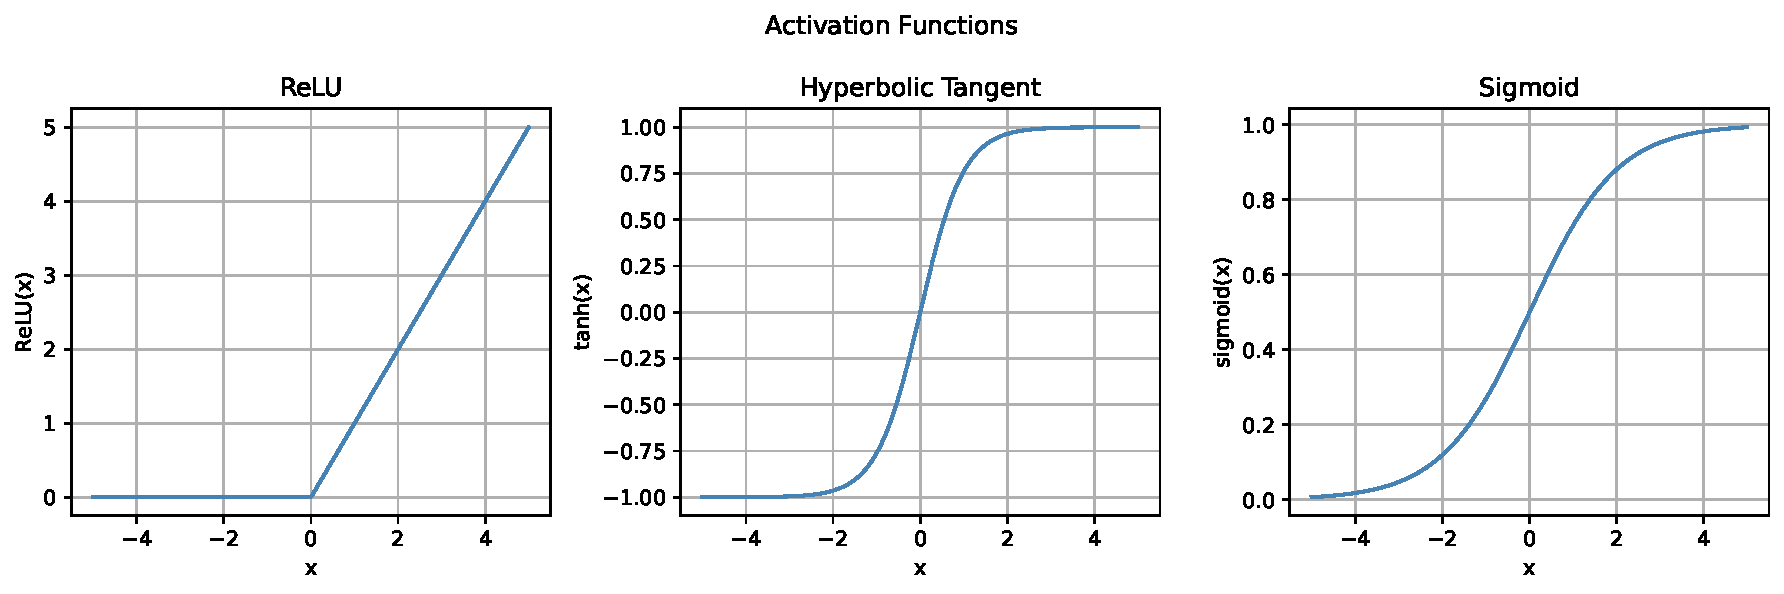
\includegraphics[width=0.9\textwidth]{Bilder/activation_functions.pdf}
        \caption{Common activation functions used in neural networks: ReLU, Hyperbolic Tangent (tanh), and Sigmoid \cite{activation}.}
        \label{fig:activation_functions}
    \end{figure}
\FloatBarrier

The sigmoid activation function $\sigma(\cdot)$ is defined as
\begin{equation}
\sigma(z) = \frac{1}{1+e^{-z}}.
\end{equation}

The forward pass proceeds in two stages. In the hidden layer, pre-activations $z_{h_1}$ and $z_{h_2}$ are computed as affine transformations of the input and mapped to activations $h_1$ and $h_2$ using $\sigma(\cdot)$. The output layer then computes $z_o$ from $h_1$ and $h_2$, and applying $\sigma(\cdot)$ yields the prediction $\hat{y} \in (0,1)$. All weights $\{w_i\}$ and bias terms $\{b_i\}$ are learned by minimizing a loss function.

\begin{align}
z_{h_1} &= w_1 x_1 + w_2 x_2 + b_1, & h_1 &= \sigma(z_{h_1}) \\
z_{h_2} &= w_3 x_1 + w_4 x_2 + b_2, & h_2 &= \sigma(z_{h_2}) \\
z_o &= w_5 h_1 + w_6 h_2 + b_3, & \hat{y} &= \sigma(z_o)
\end{align}

The quality of a prediction is measured using a loss function, which quantifies the discrepancy between the predicted output and the true target. 

\begin{equation}
\mathcal{L}_{\mathrm{BCE}}(y,\hat{y}) = -\left[y \log(\hat{y}) + (1-y)\log(1-\hat{y})\right].
\label{eq:bce}
\end{equation}

\begin{equation}
\mathcal{L}_{\mathrm{MSE}}(y,\hat{y}) = \frac{1}{2}\,(y-\hat{y})^2.
\label{eq:mse}
\end{equation}

Common loss functions include binary cross-entropy (BCE) loss defined in Equation~\eqref{eq:bce} for classification tasks and mean squared error for regression problems defined in Equation~\eqref{eq:mse}. The loss function provides the optimization objective that guides the learning process \cite{elharrouss2025taskbasedlossfunctionscomputer}.
This forward propagation process defines a differentiable mapping from inputs to outputs, enabling the network parameters to be optimized via gradient-based learning methods. In the binary classification setting with a sigmoid output, combining the BCE loss with $\hat{y}=\sigma(z_o)$ yields a particularly simple gradient expression that is used in the backpropagation derivation.

\subsection{Backpropagation and Gradient-Based Optimization}

Backpropagation is the core algorithm used to train neural networks. It computes gradients of the loss function with respect to all model parameters by recursively applying the chain rule in a backward pass through the network. These gradients indicate how each parameter should be adjusted in order to minimize the loss function \cite{RAZAVI2021105159}.

The derivative of the sigmoid activation function is given by
\begin{equation}
\sigma'(z) = \sigma(z)\bigl(1-\sigma(z)\bigr).
\end{equation}

For the output layer, the error term is defined as the derivative of the loss with respect to the pre-activation value $z_o$. When using a sigmoid activation function in combination with the binary cross-entropy loss, this term simplifies to
\begin{equation}
\delta_o \;\triangleq\; \frac{\partial \mathcal{L}}{\partial z_o}
= \hat{y} - y.
\end{equation}

The error terms for the hidden layer neurons are obtained by propagating the output error backward through the network:
\begin{align}
\delta_{h_1} &= (w_5 \delta_o)\, \sigma'(z_{h_1})
= (w_5 \delta_o)\, h_1(1-h_1), \\
\delta_{h_2} &= (w_6 \delta_o)\, \sigma'(z_{h_2})
= (w_6 \delta_o)\, h_2(1-h_2).
\end{align}

Using these error terms, the gradients of the loss function with respect to the network parameters can be computed as
\begin{align}
\frac{\partial \mathcal{L}}{\partial w_1} &= \delta_{h_1} \, x_1, &
\frac{\partial \mathcal{L}}{\partial w_2} &= \delta_{h_1} \, x_2, &
\frac{\partial \mathcal{L}}{\partial b_1} &= \delta_{h_1}, \\
\frac{\partial \mathcal{L}}{\partial w_3} &= \delta_{h_2} \, x_1, &
\frac{\partial \mathcal{L}}{\partial w_4} &= \delta_{h_2} \, x_2, &
\frac{\partial \mathcal{L}}{\partial b_2} &= \delta_{h_2}, \\
\frac{\partial \mathcal{L}}{\partial w_5} &= \delta_o \, h_1, &
\frac{\partial \mathcal{L}}{\partial w_6} &= \delta_o \, h_2, &
\frac{\partial \mathcal{L}}{\partial b_3} &= \delta_o.
\end{align}

Model parameters are updated iteratively using gradient-based optimization methods. In its simplest form, gradient descent updates each parameter $\theta$ according to
\begin{equation}
\theta \leftarrow \theta - \eta \frac{\partial \mathcal{L}}{\partial \theta},
\end{equation}
where $\eta$ denotes the learning rate. More advanced optimization algorithms, such as stochastic gradient descent with momentum, Adam, or RMSProp, adapt the learning rate dynamically to improve convergence speed and training stability, particularly in deeper network architectures \cite{sun2019optimizationdeeplearningtheory}.

In deep networks, gradients can vanish or explode as they are propagated through many layers. This effect is amplified by saturating activation functions such as the sigmoid, whose derivative becomes close to zero for large positive or negative inputs, slowing learning in earlier layers. Common mitigation strategies include non-saturating activations (e.g., ReLU), careful initialization, normalization methods, and gradient clipping \cite{elharrouss2025taskbasedlossfunctionscomputer}.

\subsection{Model Training and Evaluation}

Model training involves iteratively updating network parameters using labeled training data until convergence or until a predefined stopping criterion is met. To assess model performance and generalization capability, datasets are commonly divided into training, validation, and test sets.

Training is typically performed over multiple \emph{epochs}, where one epoch corresponds to a full pass over the training dataset. Parameters are updated in \emph{iterations} (or steps), commonly using \emph{mini-batches} of size $B$ rather than the full dataset to reduce computational cost and to obtain more frequent updates. This yields stochastic or mini-batch gradient descent updates, 
which are the standard training regime for modern neural networks \cite{hammad2024artificialneuralnetworkdeep}.

Evaluation metrics depend on the specific task and provide quantitative measures of model performance. For binary classification problems, commonly used metrics include accuracy, precision, recall, and the F1-score, which are derived from the confusion matrix consisting of true positives (TP), true negatives (TN), false positives (FP), and false negatives (FN). Figure~\ref{fig:confusion_matrix} illustrates the confusion matrix structure and the corresponding metric definitions, with color coding indicating which cells contribute to each metric.

\begin{figure}[htbp]
\centering
\begin{tikzpicture}[
    cell/.style={rectangle, minimum width=2.8cm, minimum height=1.8cm, 
                 draw, align=center, font=\small},
]

\node[font=\small\bfseries] at (5.7, 3.8) {Predicted Label};
\node[font=\small, align=center] at (4.3, 3.1) {Predicted\\True};
\node[font=\small, align=center] at (7.1, 3.1) {Predicted\\False};

\node[font=\small\bfseries, rotate=90] at (0.0, 0.7) {Actual Label};
\node[font=\small, align=center, rotate=90] at (1.2, 1.6) {Actual\\True};
\node[font=\small, align=center, rotate=90] at (1.2, -0.2) {Actual\\False};

\node[cell, fill=green!25] (TP) at (4.3, 1.6) {
    \textbf{TP}\\
    \footnotesize True Positive\\
    \footnotesize (correct)};

\node[cell, fill=red!20] (FN) at (7.1, 1.6) {
    \textbf{FN}\\
    \footnotesize False Negative\\
    \footnotesize (missed)};

\node[cell, fill=orange!25] (FP) at (4.3, -0.2) {
    \textbf{FP}\\
    \footnotesize False Positive\\
    \footnotesize (false alarm)};

\node[cell, fill=green!25] (TN) at (7.1, -0.2) {
    \textbf{TN}\\
    \footnotesize True Negative\\
    \footnotesize (correct)};

\node[align=left, font=\small] at (12.5, 2.4) {
    $\mathrm{Accuracy} = \dfrac{
        \textcolor{green!60!black}{\mathbf{TP}} + 
        \textcolor{green!60!black}{\mathbf{TN}}}{
        \textcolor{green!60!black}{\mathbf{TP}} + 
        \textcolor{green!60!black}{\mathbf{TN}} + 
        \textcolor{orange!80!black}{\mathbf{FP}} + 
        \textcolor{red!70!black}{\mathbf{FN}}}$};

\node[align=left, font=\small] at (12.5, 1.1) {
    $\mathrm{Precision} = \dfrac{
        \textcolor{green!60!black}{\mathbf{TP}}}{
        \textcolor{green!60!black}{\mathbf{TP}} + 
        \textcolor{orange!80!black}{\mathbf{FP}}}$};

\node[align=left, font=\small] at (12.5, -0.2) {
    $\mathrm{Recall} = \dfrac{
        \textcolor{green!60!black}{\mathbf{TP}}}{
        \textcolor{green!60!black}{\mathbf{TP}} + 
        \textcolor{red!70!black}{\mathbf{FN}}}$};

\node[align=left, font=\small] at (12.5, -1.4) {
    $\mathrm{F1} = 2 \cdot \dfrac{
        \mathrm{Precision} \cdot \mathrm{Recall}}{
        \mathrm{Precision} + \mathrm{Recall}}$};

\draw[dashed, gray] (9.0, -1.8) -- (9.0, 4.0);

\end{tikzpicture}
\caption{Confusion matrix for binary classification and derived evaluation metrics. \textcolor{green!60!black}{\textbf{TP}} and \textcolor{green!60!black}{\textbf{TN}} denote correct predictions; \textcolor{orange!80!black}{\textbf{FP}} and 
\textcolor{red!70!black}{\textbf{FN}} denote incorrect predictions.}
\label{fig:confusion_matrix}
\end{figure}

Proper evaluation using these metrics is essential for identifying overfitting, detecting potential biases in the data, and comparing alternative model architectures or training strategies \cite{raghu2020surveydeeplearningscientific}.

\subsection{Regularization Techniques}

Regularization techniques are used to prevent overfitting and improve generalization. Common approaches include L1 and L2 weight regularization, which penalize large parameter values, and dropout, which randomly disables neurons during training to encourage redundancy and robustness.

Early stopping is another effective regularization method, where training is halted once performance on a validation set stops improving. These techniques help neural networks generalize better to unseen data, especially when training data is limited or noisy \cite{hammad2024artificialneuralnetworkdeep}.

\subsection{Normalization Methods}

Normalization methods stabilize and accelerate training by reducing internal covariate shift. Feature scaling techniques such as normalization and standardization ensure that input features have comparable scales.

Batch normalization extends this idea to hidden layers by normalizing intermediate activations during training. This technique improves gradient flow, allows higher learning rates, and reduces sensitivity to parameter initialization, making deep networks easier to train \cite{RAZAVI2021105159}.

\subsection{Overfitting and Generalization}

Overfitting occurs when a model learns patterns specific to the training data that do not generalize to unseen data \cite{valdenegrotoro2022machinelearningstudentsoverfit}. This issue is particularly severe in high-capacity models trained on limited datasets.

Generalization refers to a model’s ability to perform well on new data drawn from the same or similar distributions. Achieving good generalization requires appropriate model complexity, sufficient data diversity, and effective regularization strategies. Understanding this trade-off is critical when applying deep learning models to real-world tasks such as fake news detection, where data distributions may shift over time \cite{raghu2020surveydeeplearningscientific}.

\section{Fake News and Detection}

Fake news detection is closely related to fact-checking, misinformation studies, and computational credibility assessment. While fact-checking typically focuses on verifying the truthfulness of individual claims (often short statements), fake news detection often targets longer pieces of content such as full articles or posts and aims to assess their overall trustworthiness \cite{vykopal2024generativelargelanguagemodels}. The following subsections introduce key definitions, taxonomies, and conceptual properties that are commonly used to frame fake news and its automated detection.

\subsection{Definitions and Taxonomies}

The term \emph{fake news} does not have a universally agreed definition, partly because its meaning has changed over time and it is often used rhetorically as a political label to discredit opponents. In academic contexts, definitions frequently converge on three criteria: (i) the content is false or misleading, (ii) it is presented in a news-like format, and (iii) it serves a deceptive or misleading function, even though the role of intent is debated \cite{encyclopedia2010043}. A widely used operational definition describes fake news as news-like content that is intentionally false or misleading and designed to deceive \cite{fi16080298}.

Taxonomies further distinguish different forms of fake news and related deceptive content. One common categorization includes political propaganda, fabricated stories, manipulated content (e.g., real events presented out of context), and parody or satire \cite{10704605}. Importantly, fake news is increasingly treated as a subtype of online disinformation that imitates journalistic conventions while violating epistemic and professional standards such as verification and accountability \cite{encyclopedia2010043}. These taxonomies emphasize that fake news is not a single phenomenon but a spectrum of deceptive practices that vary in their goals, presentation strategies, and modes of dissemination.

\subsection{Structure of Deceptive Content}

Fake news is often effective because it imitates the structure and appearance of legitimate journalism. This imitation can operate at multiple levels, including textual style (e.g., headline conventions and narrative flow), visual presentation (e.g. images, layout, or logos), and platform embedding (e.g., how items appear in feeds or previews). Structural similarity to real news tends to increase perceived credibility and can support wider diffusion \cite{appel-2019}.

Deception also frequently arises from \emph{composition} rather than pure fabrication. Many instances combine fabricated claims, distorted facts, half-truths, and even literally true statements placed in misleading contexts. Misleading meaning can be produced through framing, selective ordering of information, or omission of crucial context \cite{encyclopedia2010043}. As a result, fake news may be difficult to detect using purely surface-level cues, since credible structure and partially accurate content can mask deeper forms of manipulation.

\subsection{Misinformation vs. Disinformation}

A central distinction in the literature separates misinformation from disinformation. Misinformation refers to false or inaccurate information shared without intent to deceive, often caused by mistakes, negligence, or misunderstandings \cite{10704605}. Disinformation, in contrast, is intentionally false information created and disseminated to mislead, manipulate, or cause harm, and is often associated with political propaganda \cite{10704605,fi16080298}.

Fake news overlaps strongly with disinformation but cannot always be reduced to deliberate lying. Some creators may be largely indifferent to truth and primarily motivated by attention, virality, or profit (e.g., click-driven content), which complicates intent-based definitions. This distinction is especially important for automated detection systems: intent is rarely observable from text alone, and reliable intent inference is generally not feasible at scale. Consequently, practical computational definitions often focus on observable properties such as verifiability, evidentiary grounding, and violations of journalistic norms rather than psychological intent \cite{encyclopedia2010043}.

\subsection{Domain Dependence in Classification}

Fake news is highly context- and domain-dependent. Deceptive strategies, expected evidence standards, and persuasive rhetoric differ substantially across domains such as politics, public health, science, and commerce \cite{encyclopedia2010043,tong-etal-2025-generate}. In addition, the same content may be misleading for one audience but not for another, because interpretation depends on background knowledge, cultural context, and platform-specific presentation \cite{encyclopedia2010043}.

This domain dependence creates major challenges for classification systems. Models trained on one dataset or domain often exploit domain-specific cues and may fail when deployed on new topics or domains, leading to weak cross-domain generalization \cite{tong-etal-2025-generate}. Prior work has therefore explored incorporating social context (e.g., comment-reply structures and propagation patterns) and integrating external knowledge to improve robustness, although these enhancements may require additional data collection effort and system complexity \cite{tong-etal-2025-generate}. Overall, domain dependence motivates domain-aware modeling strategies and evaluation protocols that explicitly test generalization beyond the training distribution.

\subsection{Linguistic and Contextual Properties}

Linguistic analyses frequently associate fake news with sensationalism, emotional and polarized language, exaggeration, and strong certainty markers \cite{encyclopedia2010043,10704605}. However, such features are not reliable in isolation. High-quality fake news can be written in a professional tone and closely resemble legitimate reporting, while real news—especially in early reporting phases—may contain uncertainty or incomplete information \cite{encyclopedia2010043}.

Context is often decisive for deception. Misleading meaning can arise even when individual sentences are factually correct, for example when facts are selectively presented, crucial information is omitted, or content is framed to imply unsupported conclusions \cite{encyclopedia2010043}. This implies that effective detection should not be limited to sentence-level signals. Instead, models must capture discourse-level structure, pragmatic framing, and the relationship between claims and the contexts in which they are presented.

\subsection{Conceptualizing Lies in Computational Terms}

In philosophical terms, lying presupposes both knowledge of the truth and an intention to deceive. Translating this notion into automated detection is difficult because machine learning systems have no access to mental states and cannot directly observe intent \cite{encyclopedia2010043}. As a result, computational work typically reframes deception as an observable divergence from verifiable reality or from journalistic and epistemic norms.

Within fake news research, three common computational formulations can be distinguished. First, \emph{classification} assigns categorical labels (e.g., fake vs. real). Second, \emph{verification} evaluates claims against evidence, aligning closely with fact-checking pipelines. Third, \emph{credibility estimation} ranks or scores content according to trustworthiness. Recent progress in large language models has influenced all three formulations: generative models can produce richer outputs such as explanations, reasoning traces, and claim decomposition, which may improve interpretability. At the same time, LLMs may hallucinate, misinterpret claims, or provide incorrect justifications, and they may lack up-to-date knowledge without external retrieval \cite{vykopal2024generativelargelanguagemodels}.

\section{Large Language Models and Transformers}

Large language models have emerged as a dominant paradigm in natural language processing, enabling strong performance across a wide range of tasks without task-specific architectures. Their success is largely driven by advances in transformer-based architectures, large-scale pretraining, and flexible adaptation strategies such as prompting and fine-tuning. This section introduces the theoretical foundations of LLMs, focusing on their architectural components, training paradigms, and usage patterns that are relevant for fake news detection.

\subsection{Evolution of NLP Models}

Natural language processing has progressed alongside a broader change in AI: from hand-built linguistic systems to models that learn language patterns from data at scale. Early NLP work (roughly the 1950s–1970s) was dominated by symbolic and rule-based approaches. These systems relied on manually crafted grammars, pattern matching, and logic-based representations to parse text, translate sentences, or imitate dialogue (e.g., early machine translation efforts and ELIZA). While transparent and easy to interpret, rule-based systems struggled with ambiguity and variation in real-world language and did not generalize well beyond the scenarios anticipated by their designers \cite{chen2025deeplearningmachinelearning}.

Beginning in the 1980s, the field increasingly adopted probabilistic and statistical techniques to overcome these limitations. Classic statistical language models—especially n-gram models—estimated word probabilities from corpus statistics but were limited by short context windows and strong independence assumptions \cite{zhao2025surveylargelanguagemodels}. Even when effective for narrow tasks, these models suffered from sparsity and could not capture long-range dependencies reliably. During the 1990s, supervised machine learning further expanded NLP capabilities, supported by larger datasets and the growing availability of labeled corpora \cite{chen2025deeplearningmachinelearning}.

A major shift occurred in the 2010s with neural language models. Distributed representations (word embeddings) and end-to-end learning enabled models to capture linguistic regularities directly from data. Sequence models such as RNNs and LSTMs improved the ability to represent contextual dependencies, but they remained difficult to parallelize and scale efficiently. Transformer architectures changed this by replacing recurrence with attention, allowing much larger models to be trained effectively \cite{chen2025deeplearningmachinelearning}.

This development led to the pretraining paradigm that dominates modern NLP: large-scale self-supervised learning on general text, followed by task adaptation through fine-tuning or prompting. Large language models extend this approach by further increasing model capacity and training data, yielding strong zero-shot and few-shot performance across many tasks. As a result, NLP has shifted away from building separate task-specific systems and toward general-purpose models that can be adapted across domains with minimal additional supervision \cite{zhao2025surveylargelanguagemodels}.

\subsection{Transformer Architecture and Attention Mechanisms}

The Transformer architecture forms the foundation of modern large language models, including the LLaMA family used in this thesis. Unlike recurrent or convolutional architectures, transformers process entire token sequences in parallel, enabling efficient training and scalability to very large datasets \cite{vaswani2023attentionneed}.

A transformer layer consists of two main components: a multi-head self-attention mechanism and a position-wise feed-forward network. These components are combined with residual connections and layer normalization to stabilize training and enable deep architectures \cite{vaswani2023attentionneed}. By stacking multiple such layers, transformers can model complex, long-range dependencies within text, which is essential for reasoning-intensive tasks \cite{naveed2024comprehensiveoverviewlargelanguage}. Figure~\ref{fig:transformer-architecture} shows the original encoder--decoder Transformer architecture. The encoder (left) and decoder (right) are each composed of \(N\) stacked layers, where each layer combines multi-head attention and a position-wise feed-forward network, wrapped with residual connections and layer normalization (``Add \& Norm''). The decoder applies masked self-attention so that each token can only use information from earlier tokens, then uses encoder--decoder attention to incorporate the encoder representations, and finally outputs token probabilities via a linear layer and a softmax.

\begin{figure}[htbp]
    \centering
    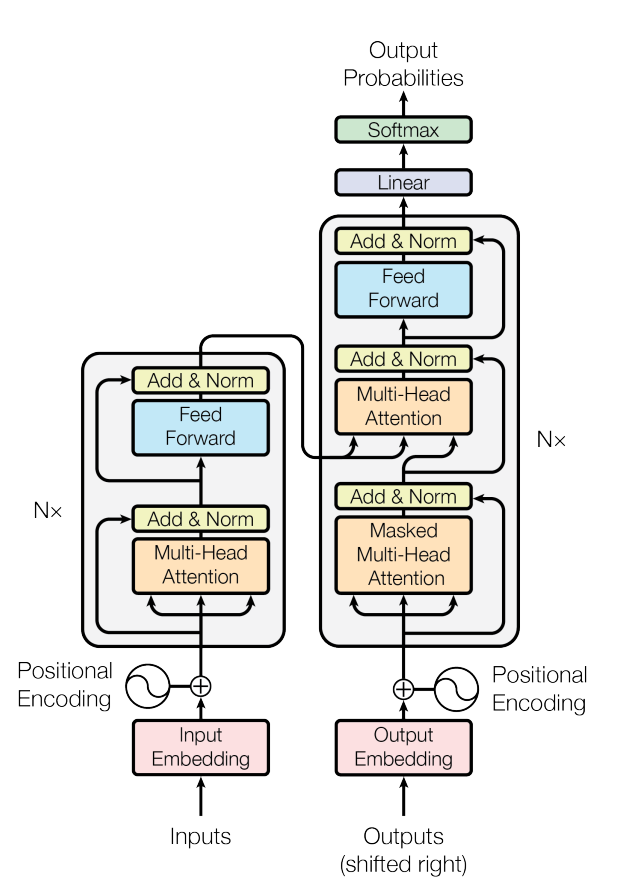
\includegraphics[width=0.4\textwidth]{Bilder/Transformer.png}
    \caption{Transformer model architecture (encoder–decoder) with the encoder shown on the left and the decoder on the right, as introduced by Vaswani et al.~\cite{vaswani2023attentionneed}.}
    \label{fig:transformer-architecture}
\end{figure}

Self-attention allows each token to attend to all other tokens in the sequence, weighting their relevance dynamically based on learned similarity scores \cite{vaswani2023attentionneed}. This enables the model to integrate contextual information regardless of token distance. Figure~\ref{fig:self_attention} illustrates the scaled dot-product self-attention computation for a single head. The input token embeddings \(X\) (here shown for the tokens \emph{``I''}, \emph{``love''}, \emph{``tennis''}) are linearly projected using learned weight matrices \(W_Q\), \(W_K\), and \(W_V\) to form queries \(Q=XW_Q\), keys \(K=XW_K\), and values \(V=XW_V\). Attention scores are computed as \(QK^\top/\sqrt{d_k}\) and normalized with a softmax to obtain the attention weight matrix \(S\). Multiplying these weights with the values (\(SV\)) produces the attention output, i.e. context-aware token embeddings where each token aggregates information from other tokens according to its learned relevance weights.

Multi-head attention extends this mechanism by computing several attention distributions in parallel, allowing the model to capture different types of relationships, such as syntactic structure or semantic relevance, within the same layer \cite{devlin2019bertpretrainingdeepbidirectional}.

\begin{figure}[htbp]
    \centering
    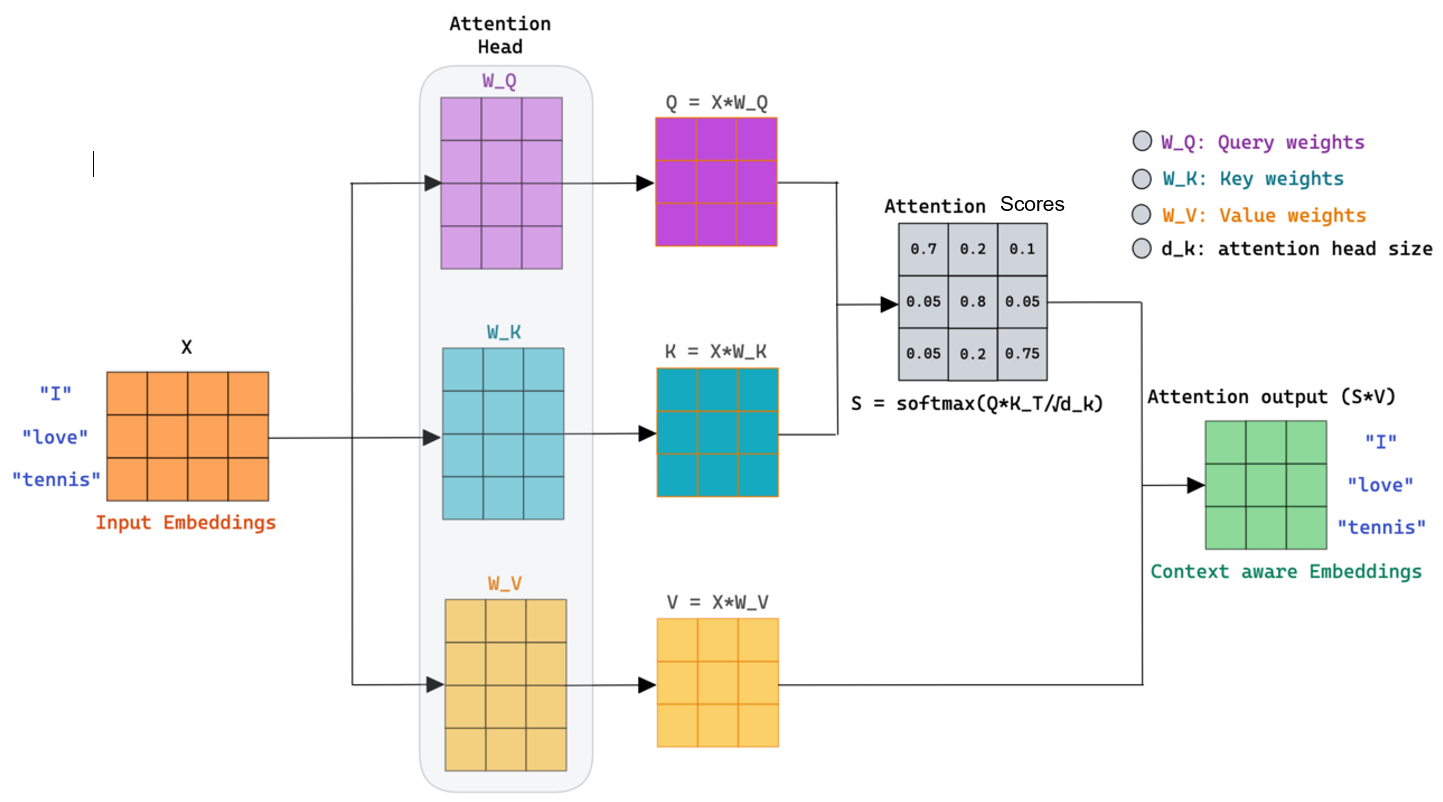
\includegraphics[width=0.9\textwidth]{Bilder/self_attention_thumbnail_corrected.png}
    \caption{Scaled dot-product self-attention (single head). Multi-head attention repeats this computation in parallel across multiple heads and concatenates the results \cite{pachaar-2025}.}
    \label{fig:self_attention}
\end{figure}

Because transformers process tokens simultaneously, they do not inherently encode word order. Positional information is therefore injected into the model using positional encodings \cite{vaswani2023attentionneed}. These encodings enable the model to distinguish between different token positions and to capture sequential structure, which is critical for tasks involving logical flow, temporal relations, or argument structure \cite{naveed2024comprehensiveoverviewlargelanguage}.

Decoder-only transformer models, such as LLaMA, employ causal self-attention masks that restrict each token to attending only to previous tokens in the sequence \cite{brown2020languagemodelsfewshotlearners}. This design supports autoregressive generation and allows the same architecture to be used for both input conditioning and output generation. Due to their architectural simplicity and strong performance in prompt-based settings, decoder-only transformers have become the dominant architecture for large language models \cite{touvron2023llamaopenefficientfoundation}.

\subsection{Tokenization and Embeddings}

Before text can be processed by a transformer, it must be converted into a sequence of tokens. Modern LLMs typically rely on subword tokenization methods, such as Byte Pair Encoding or related variants, which balance vocabulary size and expressiveness while mitigating out-of-vocabulary issues \cite{chen2025deeplearningmachinelearning}.

Each token is mapped to a continuous vector representation, known as an embedding. These embeddings serve as the initial input to the transformer and are learned during training \cite{chen2025deeplearningmachinelearning}. Embeddings enable the model to represent semantic and syntactic relationships between tokens in a continuous space, forming the basis for higher-level language understanding.

\subsection{Encoder--Decoder vs. Decoder-Only Models}

Transformer-based models can be broadly categorized into encoder--decoder architectures and decoder-only architectures. Encoder--decoder models consist of separate encoder and decoder components, where the encoder processes the input sequence and the decoder generates the output conditioned on the encoder representation. This architecture is commonly used for sequence-to-sequence tasks such as translation \cite{zhao2025surveylargelanguagemodels}.

Decoder-only models, in contrast, use a single transformer stack with causal attention masks, enabling autoregressive text generation. This architecture underlies most modern large language models and has demonstrated strong performance in zero-shot and few-shot settings \cite{naveed2024comprehensiveoverviewlargelanguage}. Decoder-only models are particularly relevant for prompt-based fake news detection, as both input and output can be handled within a single model.

\subsection{Representative LLM Families}

Several families of large language models have been proposed, differing in architecture, training strategy, and scale. Examples include instruction-tuned models, multilingual models, and mixture-of-experts architectures that activate only a subset of parameters during inference \cite{naveed2024comprehensiveoverviewlargelanguage}. These design choices aim to balance performance, efficiency, and generalization.

Despite architectural differences, most LLMs share a common foundation: transformer-based modeling, large-scale pretraining on diverse text corpora, and adaptation through prompting or fine-tuning. These shared characteristics enable comparative evaluation across models in downstream tasks such as fake news detection.

\subsection{Pretraining and Fine-Tuning Paradigms}

Large language models are typically pretrained using self-supervised objectives on large unlabeled text corpora, allowing them to acquire broad linguistic and world knowledge without task-specific supervision \cite{zhao2025surveylargelanguagemodels}. Since pretraining on billions of tokens is prohibitively expensive, the dominant paradigm reuses these pretrained weights and adapts them to downstream tasks through fine-tuning -- a second training phase on smaller, task-specific labeled datasets \cite{naveed2024comprehensiveoverviewlargelanguage}. This two-stage approach combines the broad generalization of pretraining with the precision of task-specific supervision.

\paragraph{Supervised Fine-Tuning (SFT).}
Supervised fine-tuning (SFT) is the most direct form of task adaptation. Given a labeled dataset of input--output pairs, the model is trained to minimize a task-specific loss, typically cross-entropy over the target tokens. In instruction-following settings, inputs are formatted as natural language prompts and outputs as expected completions, encouraging the model to follow instructions reliably \cite{zhao2025surveylargelanguagemodels}. SFT has been shown to substantially improve task-specific performance compared to zero-shot prompting, particularly for classification tasks with well-defined output formats.

\paragraph{Instruction Fine-Tuning.}
Instruction fine-tuning extends SFT by training on a diverse mixture of tasks formatted as natural language instructions. This approach improves generalization to unseen tasks and enhances instruction-following behavior across domains \cite{naveed2024comprehensiveoverviewlargelanguage}. Models trained with instruction fine-tuning, such as FLAN-T5 and LLaMA-Instruct variants, are better aligned with user intent and typically outperform base models in zero-shot and few-shot settings.

\paragraph{Domain-Specific Fine-Tuning.}
Beyond general task adaptation, fine-tuning can be applied to specific topical domains by restricting the training data to domain-relevant examples. Domain-specific fine-tuning allows models to learn domain-specific patterns, terminology, and label distributions that may not be well represented in general pretraining corpora \cite{lu2024finetuninglargelanguagemodels}. However, this specialization can reduce generalization to out-of-domain examples, creating a trade-off between in-domain performance and cross-domain robustness that must be carefully managed through evaluation on held-out distributions.

\paragraph{Completion-Only Training.}
In practice, fine-tuning for classification or constrained generation tasks is often implemented in a completion-only style: the model receives a formatted prompt and is trained to generate only the target label or output, while prompt tokens are masked out in the loss computation. This approach focuses optimization on the decision-relevant part of the output and avoids the model wasting capacity on reproducing the input \cite{naveed2024comprehensiveoverviewlargelanguage}.

\subsection{Parameter-Efficient Fine-Tuning with LoRA}

Fine-tuning large language models typically requires updating all model parameters, which becomes increasingly infeasible as model sizes grow. For a model such as GPT-3 with 175 billion parameters, storing and deploying separate fine-tuned instances for each downstream task is prohibitively expensive \cite{hu2021loralowrankadaptationlarge}.

Parameter-efficient fine-tuning methods address this limitation by adapting only a small subset of parameters while keeping the base model frozen. Low-Rank Adaptation (LoRA) is one such approach, proposed by Hu et al. \cite{hu2021loralowrankadaptationlarge}. The key insight behind LoRA is that the weight updates during fine-tuning have a low intrinsic rank -- that is, the change in weights $\Delta W$ can be well approximated by a low-rank decomposition.

\paragraph{Core mechanism.}
Instead of directly updating a weight matrix $W \in \mathbb{R}^{d \times d}$, LoRA freezes $W$ and injects two trainable low-rank matrices $A \in \mathbb{R}^{d \times r}$ and $B \in \mathbb{R}^{r \times d}$, where the rank $r \ll d$. The modified forward pass computes:

\begin{equation}
h = Wx + \Delta Wx = Wx + BAx,
\end{equation}

where $x$ is the input and $\Delta W = BA$ approximates the weight update. Matrix $A$ is initialized with a random Gaussian distribution and $B$ is initialized to zero, ensuring that $\Delta W = 0$ at the start of training and the model begins from the pretrained state \cite{hu2021loralowrankadaptationlarge}.

Figure~\ref{fig:lora} illustrates this reparametrization. The pretrained weights $W$ remain frozen throughout training, while only the small matrices $A$ and $B$ are updated. The number of trainable parameters is reduced from $d \times d$ to $r \times (d + d) = 2rd$, which for typical values of $r \in \{4, 8, 16\}$ and $d$ in the thousands represents a reduction of several orders of magnitude.

\begin{figure}[htbp]
\centering
\begin{tikzpicture}[
    box/.style={rectangle, rounded corners=3pt, draw, minimum width=2.0cm,
                minimum height=1.0cm, align=center, font=\small},
    frozen/.style={box, fill=gray!20, draw=gray!60},
    trainable/.style={box, fill=blue!20, draw=blue!60},
    arrow/.style={-{Stealth}, thick},
]

\node[font=\small\bfseries] at (1.5, 4.0) {Full Fine-Tuning};
\node (x_left) at (-0.3, 2.0) {$x$};
\node[frozen] (W_full) at (1.5, 2.0) {$W + \Delta W$\\\footnotesize $d \times d$};
\node (h_left) at (3.3, 2.0) {$h$};
\node[font=\footnotesize, text=red!70!black, align=center] at (1.5, 0.6) 
    {all parameters\\updated};

\draw[arrow] (x_left) -- (W_full);
\draw[arrow] (W_full) -- (h_left);

\draw[dashed, gray] (4.0, -0.8) -- (4.0, 4.5);

\node[font=\small\bfseries] at (8.0, 4.0) {LoRA};

\node (x_right) at (4.7, 2.0) {$x$};

\node[frozen, minimum width=3.0cm] (W) at (8.0, 2.8) {$W$\\\footnotesize frozen};

\node[trainable] (A) at (6.5, 0.8) {$A$\\\footnotesize $d \times r$};
\node[trainable] (B) at (9.3, 0.8) {$B$\\\footnotesize $r \times d$};

\node[font=\small, circle, draw, inner sep=1pt] (plus) at (11.0, 2.0) {$+$};
\node (h_right) at (12.3, 2.0) {$h$};

\node[font=\footnotesize, text=blue!70!black, align=center] at (8.5, -0.5) 
    {only $A$, $B$ updated\\$r \ll d$};

\draw[arrow] (x_right) |- (W.west);

\draw[arrow] (x_right) |- (A.west);

\draw[arrow] (A) -- (B);

\draw[arrow] (W.east) -| (plus.north);

\draw[arrow] (B.east) -| (plus.south);

\draw[arrow] (plus) -- (h_right);

\end{tikzpicture}
\caption{Comparison of full fine-tuning and LoRA. In full fine-tuning, all 
parameters of $W$ are updated. In LoRA, $W$ is frozen and only the low-rank 
matrices $A \in \mathbb{R}^{d \times r}$ and $B \in \mathbb{R}^{r \times d}$ 
are trained, where $r \ll d$. The weight update is approximated as 
$\Delta W = BA$ \cite{hu2021loralowrankadaptationlarge}.}
\label{fig:lora}
\end{figure}

\paragraph{Advantages.}
LoRA offers several practical benefits \cite{hu2021loralowrankadaptationlarge}:
\begin{itemize}
    \item \textbf{Storage efficiency:} Multiple task-specific adapters can share 
    a single frozen base model, with only the small $A$ and $B$ matrices stored 
    per task.
    \item \textbf{No inference latency:} At deployment time, $\Delta W = BA$ 
    can be merged into $W$, so the adapted model has the same architecture as 
    the original.
    \item \textbf{Reduced memory:} Since gradients are only computed for $A$ 
    and $B$, GPU memory requirements are substantially lower than full fine-tuning.
\end{itemize}

\subsection{Prompting Techniques}

Prompting refers to the practice of steering a language model's behavior through natural language instructions provided at inference time, rather than through explicit parameter updates. Prompts may include task descriptions, formatting constraints, or illustrative examples that influence the structure and content of the model's output \cite{naveed2024comprehensiveoverviewlargelanguage}.

Prompt-based approaches are particularly attractive in low-resource or rapidly evolving settings, as they eliminate the need for costly model retraining. However, model performance can be highly sensitive to prompt design choices, including wording, structure, and the ordering of examples. This sensitivity introduces variability in model behavior and poses challenges for reproducibility and systematic evaluation \cite{schulhoff2025promptreportsystematicsurvey}.

\paragraph{Zero-shot and few-shot prompting.}
Zero-shot prompting evaluates a model's ability to perform a task without exposure to labeled examples within the prompt. This setting reflects realistic deployment scenarios where task-specific training data is unavailable. Few-shot prompting extends this paradigm by providing a small number of input--output examples that demonstrate the desired behavior, allowing the model to infer the task format and expected output style \cite{brown2020languagemodelsfewshotlearners}.

\paragraph{Chain-of-thought prompting.}
Chain-of-thought (CoT) prompting encourages large language models to explicitly generate intermediate reasoning steps before producing a final answer. This approach has been shown to improve performance on tasks requiring multi-step reasoning, as the model is guided to decompose complex problems into smaller, more tractable steps. In the context of fact-checking, CoT prompting can encourage models to articulate evidence-based justifications before committing to a binary verdict, potentially improving both accuracy and interpretability \cite{wei2023chainofthoughtpromptingelicitsreasoning}.

\paragraph{Self-consistency and iterative prompting.}
Beyond single-pass prompting, more sophisticated strategies aggregate predictions across multiple prompt variants or apply staged prompting based on model confidence. Self-consistency samples multiple reasoning paths and selects the most consistent answer via majority voting, reducing variance from prompt sensitivity. Reprompting applies a second-stage prompt when the model's confidence falls below a threshold, encouraging reconsideration of uncertain cases \cite{wang2023selfconsistencyimproveschainthought}. 

\paragraph{Prompt sensitivity and structured output constraints.}
A recurring challenge in prompt-based evaluation is the high sensitivity of model outputs to prompt phrasing, formatting, and label representation. Small changes in wording can lead to substantially different predictions, making systematic comparison across models difficult \cite{schulhoff2025promptreportsystematicsurvey}.

While large language models have demonstrated strong few-shot learning capabilities, in some cases approaching the performance of fully fine-tuned models, prompt engineering alone often remains insufficient for robust classification in domain-specific settings, motivating the combination of prompting with supervised adaptation and structured reasoning mechanisms \cite{schulhoff2025promptreportsystematicsurvey}.

\section{Multi-Agent Systems in NLP}

Multi-agent systems (MAS) consist of multiple autonomous entities, called agents, that interact within a shared environment to achieve individual or collective goals. Unlike monolithic models, MAS rely on decentralization, collaboration, and coordination, which makes them well suited for complex, dynamic, and distributed problems. With the recent progress of large language models, MAS have gained renewed attention in natural language processing, where multiple language-capable agents can work together to improve reasoning, planning, and task performance \cite{tran2025multiagentcollaborationmechanismssurvey}.

\subsection{Concepts of Multi-Agent Systems}

An agent is generally defined as an autonomous entity that can perceive its environment through sensors and act upon it in order to achieve specific objectives. Agents are typically characterized by autonomy, reactivity, proactivity, and sociability, allowing them to make independent decisions while interacting with other agents or humans. Agents may be implemented as software-based, hardware-based, or hybrid systems and often operate under constraints such as limited information or computational resources \cite{8352646}.

A multi-agent system is a distributed system composed of multiple interacting agents without centralized control. Agents within a MAS cooperate, coordinate, negotiate, or compete depending on the system objectives. MAS are particularly suitable for problems that are difficult or impossible for a single agent to solve, particularly in environments that are dynamic, partially observable, or non-deterministic \cite{argoneto-2008}.

MAS are commonly described through four core components: agents, environment, interactions, and organization. The environment represents the external context in which agents are situated and may be physical or virtual. Interactions occur through communication protocols that enable knowledge sharing, coordination, and conflict resolution. Organizational structures may be hierarchical or emerge dynamically through agent interactions. The decentralized nature of MAS contributes to scalability, robustness, and fault tolerance, as system operation can continue even when individual agents fail \cite{8352646}.

\subsection{Specialized vs. Generalist Agents}

Agents within a multi-agent system may differ in their roles, capabilities, and knowledge representations. Generalist agents are designed to perform a wide range of tasks using broad knowledge and reasoning abilities, while specialized agents focus on specific subtasks or domains. In LLM-based MAS, specialization is often achieved through distinct prompts, personas, or tool access rather than separate model architectures \cite{tran2025multiagentcollaborationmechanismssurvey}.

Specialized agents enable effective division of labor by distributing subtasks across agents with complementary expertise. This approach reduces cognitive and computational load on individual agents and allows the system to pool diverse knowledge bases. As a result, MAS can achieve better generalization by combining the strengths of multiple agents rather than relying on a single monolithic model \cite{8352646}.

Generalist agents, on the other hand, provide flexibility and adaptability, particularly in open-ended or rapidly changing tasks. Hybrid systems that combine generalist coordination agents with specialized task agents have shown strong performance, as they balance adaptability with efficiency. Such designs are increasingly common in NLP applications that require reasoning, long-term planning, and multi-step problem solving \cite{8352646}.

Frameworks such as AutoGen and CAMEL illustrate how specialization can be achieved in LLM-based multi-agent systems through role assignment rather than architectural changes \cite{wang2025rethinkingmultiagentintelligencelens}. In AutoGen, agents are organized into conversational roles that coordinate planning, execution, and verification, while CAMEL employs role-playing prompts to induce cooperative behavior between agents \cite{wu2023autogenenablingnextgenllm, li2023camelcommunicativeagentsmind}. These approaches demonstrate that specialized agent roles can significantly enhance reasoning and task performance without requiring model fine-tuning.

\subsection{Collaboration and Decision Strategies}

Collaboration is a defining characteristic of multi-agent systems and enables agents to collectively solve complex tasks. Agents coordinate by sharing information, delegating subtasks, and aligning their actions toward shared objectives. In LLM-based MAS, collaboration often takes the form of structured communication channels, including debates, critiques, and iterative refinement of solutions \cite{wang2025rethinkingmultiagentintelligencelens}.

Decision-making strategies in MAS may be centralized, decentralized, or emergent. Decentralized decision-making allows agents to act autonomously based on local observations and shared knowledge, enhancing robustness and scalability. Agents may employ learning mechanisms to adapt their behavior over time, leading to systems known as multi-agent learning (MAL) systems. These systems often draw on concepts from game theory, where agents aim to optimize individual or collective rewards through repeated interactions \cite{app9071402}.

Recent studies highlight the importance of communication topology in collaborative MAS. While early approaches favored fully connected communication graphs, later work demonstrates that structured or sparse topologies, such as ring-based communication, can achieve comparable or superior performance with reduced communication overhead. This suggests that unrestricted information sharing may introduce noise or error propagation, whereas constrained interaction can improve coordination efficiency \cite{wang2025rethinkingmultiagentintelligencelens}.

\subsection{Applications in NLP}

Multi-agent systems have demonstrated notable successes across a variety of NLP tasks by enhancing the capabilities of individual language models through collaboration and coordination. Applications include complex question answering, multi-step reasoning, text generation, planning, and dialogue systems. By distributing tasks among agents, MAS enable parallel processing, long-term planning, and persistent problem-solving over extended interactions \cite{tran2025multiagentcollaborationmechanismssurvey}.

In few-shot and zero-shot settings, MAS leverage collaborative reasoning to compensate for limited supervision. Agents may critique each other’s outputs, propose alternative interpretations, or refine intermediate results, leading to improved accuracy and reliability. Multi-agent debate frameworks exemplify this approach, where agents iteratively exchange arguments to converge on higher-quality solutions as illustrated in Figure~\ref{fig:NLP_Application} \cite{wei2023chainofthoughtpromptingelicitsreasoning}.

Beyond performance improvements, MAS offer advantages in robustness, scalability, and adaptability. Decentralized control allows systems to continue functioning under partial failures, while self-organization enables dynamic task allocation in changing environments. These properties make MAS particularly suitable for real-time and large-scale NLP applications, such as conversational assistants, decision-support systems, and collaborative AI platforms \cite{tran2025multiagentcollaborationmechanismssurvey}.

    \begin{figure}[htbp]
        \centering
        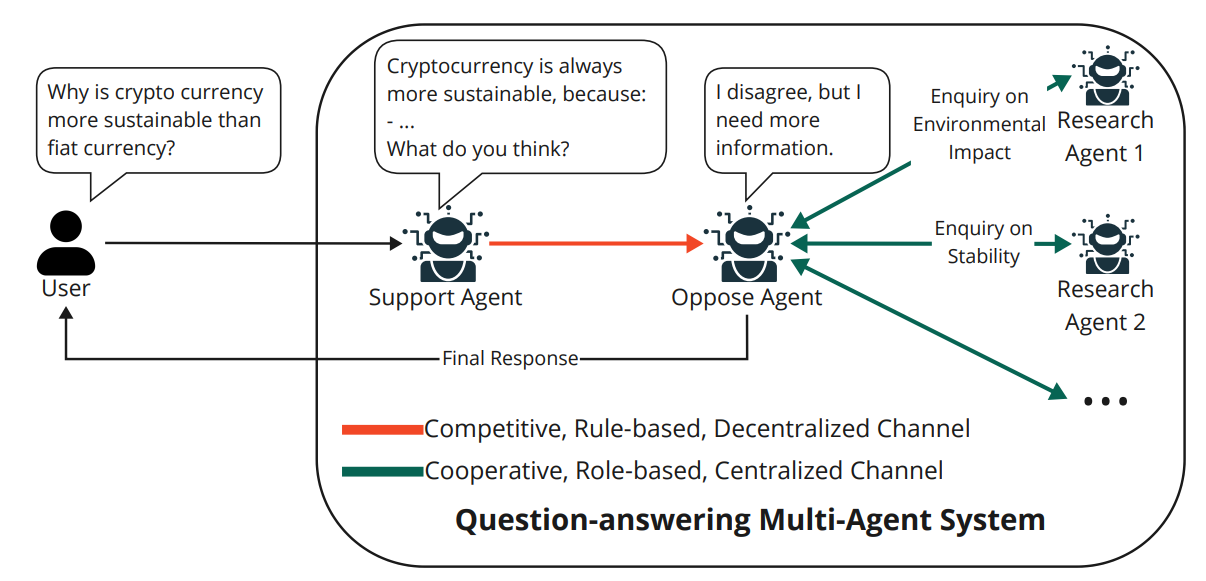
\includegraphics[width=0.9\textwidth]{Bilder/NLP_Application.png}
        \caption{Illustration of a question-answering multi-agent system as an example of agent collaboration and competition. Specialized agents interact through two communication channels: a competitive, rule-based, decentralized channel (red) and a cooperative, role-based, centralized channel (green), producing a final response to the user query \cite{tran2025multiagentcollaborationmechanismssurvey}.}
        \label{fig:NLP_Application}
    \end{figure}
    \FloatBarrier
  \chapter{Related Work}

This chapter surveys prior work on automated fake news detection and situates this thesis within the existing literature. The review is organized around three core directions relevant to this work: (i) deep learning and LLM-based detection, (ii) domain-aware and 
evidence-grounded classification, and (iii) agentic and multi-agent systems. For each direction, key contributions are summarized and their limitations identified. The chapter concludes by identifying the research gap that this thesis addresses.

\section{Deep Learning and LLM-Based Detection}

Early fake news detection systems relied on manually engineered linguistic and psychological features combined with classical machine learning classifiers such as logistic regression and support vector machines. While effective on early benchmarks, these approaches suffered from limited generalization and vulnerability to sophisticated misinformation strategies. Neural network-based models, including convolutional and recurrent architectures, improved representation learning by capturing contextual and sequential information. The introduction of pre-trained language models such as BERT further advanced detection performance by enabling contextualized text understanding, and hybrid models combining LLM representations with neural classifiers achieved strong results across multiple benchmarks \cite{10.1145/3728725.3728739}.

More recent research explores the direct use of LLMs for misinformation detection. However, studies show that misinformation generated by LLMs is often harder for both humans and automated detectors to identify than human-written misinformation with equivalent semantics, revealing critical weaknesses in existing detection systems \cite{chen2024llmgeneratedmisinformationdetected}. To address data scarcity and class imbalance, some approaches use LLMs to generate synthetic fake news examples and apply reinforcement learning-based sampling strategies, achieving substantial improvements in detection performance \cite{tong-etal-2025-generate}.

Several studies also highlight limits of text-only classification. Diagnostic evaluations on political claim benchmarks suggest a performance ceiling for fine-grained veracity prediction when models rely mostly on lexical or shallow semantic cues \cite{hasan2025generalizationgapspoliticalfake}. Work in applied settings similarly shows that textual signals often dominate prediction, while simple metadata features can still help when language models are not available or computation is limited \cite{savatteri2025signalsreallymattermisinformation}. Together, these findings motivate approaches that incorporate external evidence and focus on robustness, instead of relying only on monolithic content classifiers.

\section{Domain-Aware and Evidence-Grounded Classification} 

Misinformation characteristics vary significantly across domains such as politics, healthcare, and finance, motivating domain-aware and evidence-based detection approaches. Many systems incorporate external knowledge sources, document-level evidence, knowledge graphs, and credibility cues to improve factual verification. Knowledge-enhanced models and graph-based approaches are particularly effective in high-stakes domains by modeling entity--fact relationships and source credibility \cite{10.1145/3728725.3728739}. 

Beyond static knowledge integration, document-grounded factuality checking has emerged as a core component for verifying LLM outputs and detecting misinformation claims. Efficient fact-checkers such as MiniCheck demonstrate that small, specialized sequence-to-sequence models can approximate large-model verification quality when trained on high-quality synthetic errors, reducing inference cost and latency while remaining evidence-grounded \cite{tang-etal-2024-minicheck}. In parallel, modular toolkits and unifying frameworks (e.g., OpenFactCheck) aim to standardize the construction and evaluation of fact-checking pipelines and LLM factuality assessment, improving comparability across methods \cite{wang2025openfactcheckbuildingbenchmarkingcustomized}. Survey work further consolidates this space by categorizing how generative LLMs are used across the fact-checking pipeline, including evidence retrieval, claim verification, and synthetic data generation \cite{vykopal2024generativelargelanguagemodels}. 

Domain-specific pipelines also increasingly combine retrieval quality signals with selective reasoning. In health misinformation, two-stage systems first estimate agreement or stance across retrieved evidence and only trigger more expensive multi-agent deliberation when evidence is conflicting or uncertain, improving efficiency while maintaining accuracy \cite{chen2025exploringhealthmisinformationdetection}. More generally, confidence-aware routing approaches argue that retrieval should be invoked adaptively (rather than indiscriminately), using signals such as probabilistic certainty and reasoning consistency to decide between internal knowledge, targeted retrieval, or deeper search \cite{wang2026factcheckinglargelanguagemodels}. 

\section{Multi-Agent, Agentic, and Ensemble Approaches} 

To overcome limitations of monolithic detection systems, recent work has explored agentic and multi-agent frameworks for misinformation detection and fact-checking. Single-agent pipelines such as FactAgent simulate expert fact-checking workflows by decomposing verification into multiple structured reasoning steps, including internal knowledge checks and external evidence retrieval. These systems improve transparency and performance without requiring supervised training \cite{li2024largelanguagemodelagent}. 

Multi-agent systems extend this paradigm by assigning specialized roles to multiple agents that collaborate or compete to assess a claim's veracity. Debate-based frameworks such as TruEDebate frame fake news detection as a structured argumentative process, where agents generate opposing arguments and synthesis agents aggregate them into a final decision, improving robustness and interpretability \cite{10.1145/3726302.3730092}. Other multi-agent frameworks adopt modular architectures spanning the misinformation lifecycle, including detection, correction, source verification, and provenance tracking \cite{gautam2025multiagentsystemsmisinformationlifecycle}. Logical and causal reasoning can also be explicitly introduced via specialized agent roles (e.g., counterfactual or causal evaluators) to detect inconsistencies and improve reasoning transparency \cite{10.1145/3696410.3714748}. Relatedly, distributed decision formulations study how to aggregate labels from multiple imperfect agents by learning agent reliabilities over time, connecting misinformation verification to online learning and crowdsourcing-style aggregation \cite{verma2025multiagentfactchecking}. 

A recurring theme in agentic systems is the tight coupling between debate and retrieval. Tool-augmented debate frameworks equip different agents with heterogeneous tools (e.g., web search vs.\ curated RAG corpora) and iteratively refine queries as the debate evolves, reducing hallucinations and improving grounding \cite{jeong2026toolmadmultiagentdebateframework}. Similar ideas appear in zero-shot fake news detection under knowledge cutoff constraints: retrieval is driven by entity-based query generation, followed by multi-LLM role-based interaction and adjudication to produce interpretable verdicts \cite{wu2025zofiazeroshotfakenews}. For multimodal and real-world settings, evidence-grounded, multi-persona agentic frameworks further combine web evidence, reverse image search, and knowledge graph paths, often paired with a lightweight classifier to mitigate LLM uncertainty \cite{bukke2025agenticmultipersonaframeworkevidenceaware}. 

\section{Robustness, Adversarial Misinformation, and Style Invariance} 

As adversaries increasingly mimic credible writing style and exploit generative models, robustness has become a central concern. Empirical evidence suggests LLM-generated misinformation can evade both human judgment and automated detectors more effectively than comparable human-written misinformation \cite{chen2024llmgeneratedmisinformationdetected}. To reduce reliance on style cues, several methods shift toward content-grounded or event-centric representations. For example, FACTGUARD extracts event-centric content using LLMs and applies a reliability mechanism to down-weight contradictory or unclear advice; it also includes a distilled variant for resource-constrained deployment \cite{he2025factguardeventcentriccommonsenseguidedfake}. Complementarily, adversarial co-evolution frameworks such as RADAR train a generator to produce harder fake variants via factual perturbations while improving a retrieval-augmented detector, using natural-language critiques (verbal adversarial feedback) to strengthen robustness beyond scalar reward signals \cite{ma2026radarretrievalaugmenteddetectoradversarial}. 

\section{Multimodality, Propagation, Early Detection, and Fine-Grained Benchmarks} 

Real-world misinformation is often multimodal and time-sensitive. Multimodal systems integrate text with images and other contextual signals to detect cross-modal inconsistencies and improve robustness \cite{10.1145/3728725.3728739}. Early detection is especially challenging because propagation signals may not yet be observable; recent agent-driven approaches address this by simulating early diffusion patterns (`virtual propagation'') with role-differentiated LLM agents and fusing the simulated social evidence with content signals, improving performance in cold-start stages \cite{gu2026aheadspreadagentdrivenvirtual}. 

Finally, newer benchmarks highlight that binary document-level labels can hide fine-grained falsity patterns. Span-level datasets such as MisSpans annotate which exact spans are false within sentences and categorize misinformation types, enabling more actionable explanations and revealing that fine-grained localization remains difficult for current LLMs even when coarse classification appears strong \cite{liu2026misspansfinegrainedfalsespan}. Related benchmark work also targets ambiguity in intent, such as distinguishing satire from fake news, and shows that lightweight transformer models can be competitive while emphasizing calibration and statistical testing \cite{chhetri2025wisewebinformationsatire}. 

\section{Evaluation Frameworks and End-to-End Fact-Checking Assessment} 

Beyond model architectures, evaluation methodology strongly shapes conclusions. Arena-style evaluation frameworks benchmark end-to-end fact-checking pipelines (claim extraction/decomposition, tool-augmented retrieval, and justification-driven verdict prediction) and show that strong claim-level accuracy may not translate into full-pipeline competence \cite{lin2026comprehensivestagewisebenchmarkinglarge}. Similarly, adaptive evaluation approaches generate model-centric test cases iteratively to probe reasoning quality and justification faithfulness beyond static benchmarks \cite{lin-etal-2025-fact}. In applied political fact-checking, large-scale studies indicate that web-search or reasoning modes yield only modest gains unless retrieval is curated and claim-specific, underscoring the importance of retrieval quality and evaluation design \cite{deverna2025largelanguagemodelsrequire}. 

Overall, recent trends move from monolithic text classifiers toward evidence-grounded and agentic systems that integrate retrieval, 
specialized reasoning roles, and calibrated decision aggregation. While these approaches improve interpretability and robustness, they also introduce new challenges in coordination complexity, cost, and trustworthy reporting of evidence and system success 
\cite{DBIS2025,chen2025evidenceboundautonomousresearchevibound}. Despite this progress, several gaps relevant to short political claim verification remain, which are addressed in the following section.

\section{Research Gap and Positioning of This Thesis}

Despite substantial progress, several important gaps remain in the existing literature. First, most LLM-based detection systems are 
evaluated on general or long-form content and do not specifically address the challenges of short political claims, where the veracity signal is weak and domain-specific knowledge is critical. Second, while domain-aware approaches have been explored, few studies systematically investigate how different levels of domain granularity affect both in-domain performance and cross-domain generalization on a political fact-checking benchmark such as LIAR. Third, existing multi-agent systems for fact-checking predominantly rely on external retrieval or web search, whereas the feasibility and effectiveness of retrieval-free, domain-specialized multi-agent architectures remains underexplored.

This thesis addresses these gaps by systematically investigating binary claim verification on the LIAR benchmark using retrieval-free LLM-based approaches. Concretely, it evaluates how domain knowledge incorporated through prompting, fine-tuning, and agent specialization affects classification accuracy and cross-domain generalization (RQ1a, RQ1b), and whether multi-agent architectures with domain routing and aggregation mechanisms outperform single-model baselines in this setting (RQ2). Unlike most prior work, this thesis focuses on the interaction between domain specialization and multi-agent coordination without relying on external evidence retrieval, making it directly comparable to prior prompt-based and fine-tuning baselines on the same benchmark.
  \chapter{Dataset and Problem Setup}

\section{LIAR Dataset}
\subsection{Dataset Structure and Labels}

This thesis addresses binary claim verification: given a short political statement, the task is to classify it as either \texttt{true} or \texttt{false}. The LIAR dataset serves as the primary benchmark for all experiments.
The LIAR dataset is a widely used benchmark for fake news detection and political fact-checking \cite{wang2017liarliarpantsfire}. It consists of short statements collected from PolitiFact, each annotated with a fine-grained truthfulness rating assigned by professional fact-checkers. The dataset contains six labels: \textit{pants-fire}, \textit{false}, \textit{barely-true}, \textit{half-true}, \textit{mostly-true}, and \textit{true}.

Each statement is accompanied by rich metadata, including the speaker’s name, political affiliation, role, geographic location, topic categories, and a historical credibility profile summarizing prior PolitiFact ratings. This auxiliary information enables experiments that go beyond text-only classification and supports research on speaker-based and context-aware detection approaches \cite{wang2017liarliarpantsfire}.

Importantly, LIAR labels reflect journalistic assessments rather than strictly logical or factual truth values. As a result, labels may encode interpretive judgments, contextual assumptions, or evaluative criteria that are not fully recoverable from the statement text alone.

\subsection{Domains and Label Distribution}

Statements in the LIAR dataset span a wide range of political and societal domains, including government policy, elections, public finance, terrorism, public health, and social issues \cite{wang2017liarliarpantsfire}. These domains differ substantially in linguistic style, evidentiary requirements, and contextual dependencies.

The label distribution is imbalanced, with intermediate categories such as \textit{half-true} and \textit{mostly-true} occurring frequently. This reflects the nuanced nature of political discourse, where statements often mix factual and misleading elements rather than being entirely false or true \cite{wang2017liarliarpantsfire}.

Such domain and label heterogeneity increases task difficulty and makes LIAR particularly challenging for automated detection systems, especially when models are evaluated in cross-domain or domain-agnostic settings.

\subsection{Binary Label Mapping}

The original LIAR dataset provides six fine-grained truthfulness labels: \textit{pants-fire}, \textit{false}, \textit{barely-true}, 
\textit{half-true}, \textit{mostly-true}, and \textit{true}. For the experiments in this thesis, these labels are mapped to a binary scheme as follows:

\begin{table}[h]
\centering
\begin{tabular}{ll}
\toprule
Original Label & Binary Label \\
\midrule
pants-fire    & \texttt{false} \\
false         & \texttt{false} \\
barely-true   & \texttt{false} \\
\midrule
half-true     & \texttt{true} \\
mostly-true   & \texttt{true} \\
true          & \texttt{true} \\
\bottomrule
\end{tabular}
\caption{Mapping of original six-class LIAR labels to binary labels.}
\label{tab:label_mapping}
\end{table}

\paragraph{Limitations of binary reduction.}
This mapping necessarily discards fine-grained distinctions between degrees of truthfulness. In particular, statements labeled 
\textit{barely-true} and \textit{half-true} occupy an ambiguous middle ground -- both contain partial truth -- yet are assigned to opposite binary classes. This introduces label noise at the decision boundary and means that the binary task is inherently harder than it might appear, since semantically similar statements can receive opposing labels 
\cite{wang2017liarliarpantsfire}.

\paragraph{Rationale for binary classification.}
Despite this limitation, binary classification is the appropriate formulation for this thesis for three reasons. First, fine-grained 
six-class classification on LIAR is extremely difficult even for strong models, with state-of-the-art systems achieving only around 
27--30\% accuracy \cite{wang2017liarliarpantsfire}, making it unsuitable as a reliable evaluation target. Second, binary 
classification aligns with the practical objective of fact-checking systems, which must ultimately distinguish factual from non-factual claims \cite{vykopal2024generativelargelanguagemodels}. Third, reducing the label space to two classes enables a more controlled analysis of the impact of domain knowledge and multi-agent coordination, which are the central research questions of this 
thesis, without confounding effects from highly imbalanced multi-class labels \cite{hasan2025generalizationgapspoliticalfake}.

\subsection{Biases and Challenges}

Despite its popularity, the LIAR dataset exhibits several inherent limitations that affect automated fake news detection. First, many statements depend strongly on external context or implicit references. Statements containing personal pronouns or vague referents cannot be fully interpreted without detailed background knowledge, even when metadata is available \cite{wang2017liarliarpantsfire}.

Second, some entries do not constitute verifiable claims at all but merely describe topics or issues. In such cases, neither human annotators nor automated systems can reliably assess truthfulness, which introduces noise into the dataset.

Third, LIAR labels are derived from PolitiFact judgments, which may incorporate contextual framing, rhetorical emphasis, or evaluative interpretation. As a result, statements that are semantically plausible or partially correct may still receive labels such as \textit{false}. This highlights a structural mismatch between natural language understanding and journalistic fact-checking criteria \cite{wang2017liarliarpantsfire}.

Finally, the dataset contains sensitive content, including statements related to suicide or self-harm. Such content raises ethical concerns and may require special handling during preprocessing and evaluation.

In addition to these structural limitations, prior empirical studies indicate that fake news detection on the LIAR dataset is intrinsically difficult. Initial baselines reported by Wang et al.\ achieved a fine-grained classification accuracy of only 27.4\%, and subsequent work confirms that performance remains limited even with more advanced models. Notably, large pretrained language models such as RoBERTa achieve only moderate improvements on simplified binary variants, suggesting that the dataset provides a weak and ambiguous veracity signal when using text alone. These findings indicate that LIAR poses fundamental challenges for text-only fake news detection approaches \cite{hasan2025generalizationgapspoliticalfake}.

\subsection{Preprocessing}
\label{sec:preprocessing}
Prior to model evaluation, the LIAR dataset was preprocessed to simplify the input representation and reduce noise. Only the statement text, label, and high-level topical information were retained, while auxiliary metadata such as speaker identity, political affiliation, credibility counts, and contextual descriptions were removed. This decision ensures a text-focused evaluation and avoids unintended information leakage from speaker-specific or historical features.

The statement texts were further cleaned using a rule-based preprocessing pipeline. This included the removal of punctuation artifacts, emojis, hashtags, user mentions, and URLs, as well as the normalization of repeated symbols, dates, and time expressions. Common formatting inconsistencies and special characters were eliminated, and excessive whitespace was reduced. These steps aim to standardize the textual input while preserving semantic content, enabling a fair comparison across models and minimizing noise that could bias text-only fake news detection.

\subsection{ChatGPT Baseline Evaluation}
\label{sec:gold_standard_eval}

To establish a reference baseline for text-only fake news classification, an additional evaluation was conducted using ChatGPT (version 5.1 Thinking) as an external large language model. This evaluation serves as an upper-bound reference for prompt-only performance rather than defining absolute ground truth.

All statements from the test split of the LIAR dataset were manually entered into ChatGPT. Each statement was evaluated in an isolated interaction: for every sample, a new chat session was opened to prevent contextual carry-over between statements. The model was queried using the same prompt for all samples: \emph{``Is this statement true or false? Only answer with true or false.''} The default system settings of ChatGPT were used throughout the evaluation.

If the model responded with an answer other than \textit{true} or \textit{false}, the prompt was repeated once. If the model remained uncertain or produced a non-binary response after the second attempt, the prediction was recorded as \textit{unknown}. This conservative procedure was chosen to avoid forcing binary decisions in cases where the model explicitly expressed uncertainty or required additional context.

For quantitative analysis, the original six LIAR labels were mapped to a binary scheme (\textit{true} vs.\ \textit{false}). Predictions marked as \textit{unknown} were excluded from the binary metric computation, resulting in $n=1223$ evaluated samples. Table~\ref{tab:chatgpt_metrics} summarizes the main performance indicators. The model achieved an accuracy of $0.6321$ and a macro-F1 score of $0.62$. The confusion matrix (true labels as rows, predictions as columns) is
\[
\begin{bmatrix}
483 & 52\\
398 & 290
\end{bmatrix}.
\]
These results show a strong asymmetry across classes: recall for \textit{false} is high ($0.90$), while recall for \textit{true} is substantially lower ($0.42$). In other words, ChatGPT tends to label ambiguous claims as \textit{false}, which increases false negatives for the \textit{true} class.

\FloatBarrier
\begin{table}[t]
\centering
\caption{ChatGPT 5.1 Thinking performance on LIAR-Testset (binary mapping). Unknown predictions were excluded ($n=1223$).}
\label{tab:chatgpt_metrics}
\begin{tabular}{lccc}
\toprule
Class & Precision & Recall & F1 \\
\midrule
false & 0.55 & 0.90 & 0.68 \\
true  & 0.85 & 0.42 & 0.56 \\
\midrule
Accuracy & \multicolumn{3}{c}{0.6321} \\
Macro avg & 0.70 & 0.66 & 0.62 \\
Weighted avg & 0.72 & 0.63 & 0.62 \\
\bottomrule
\end{tabular}
\end{table}

These results highlight fundamental limitations of text-only large language models when applied to the LIAR dataset. In particular, statements requiring external context, speaker-specific knowledge, or nuanced interpretation of journalistic fact-checking criteria pose significant challenges. The observed performance therefore supports the motivation for domain-aware and multi-agent detection approaches that can incorporate complementary information sources and specialized reasoning strategies

\paragraph{Qualitative reference: ``Deep Research'' mode vs.\ standard mode.}

To better understand the role of retrieval-style behavior, a small qualitative comparison was run using GPT-5.1 with and without ``Deep Research'' (i.e. a mode intended to use more explicit investigation). The example-level outputs for this subset are shown in Table~\ref{tab:gpt_deep_research_examples}. On the same subset of example statements, the standard setting frequently produced confident but inconsistent labels (e.g., predicting \textit{true} for statements that are labeled \textit{false} in LIAR), and it also returned several \textit{unknown}/empty outputs despite the binary instruction. In contrast, the Deep Research setting produced more consistent binary outputs on the shown examples and reduced some obvious reversals, although it still produced occasional \textit{unknown} responses. Since this comparison was conducted only on a small set of illustrative cases (not the full test split), the results are reported as qualitative evidence rather than a quantitative benchmark.

\section{Domain Grouping}

This section introduces the domain grouping strategy applied in this thesis. Building on the exploratory analysis of fine-grained domain labels, semantically related domains are aggregated into higher-level super-categories to reduce data sparsity and improve modeling robustness. The grouping aims to preserve meaningful topical distinctions while enabling more reliable learning and evaluation across domains.

\subsection{Domain Super-Categories}

The original dataset contains a large number of fine-grained topical domains, many of which are closely related or overlapping in content. To reduce data sparsity and improve modeling robustness, the original domains were grouped into higher-level super-categories based on semantic coherence and practical relevance for misinformation detection.

Table~\ref{tab:domain_mapping} shows selected examples of how original LIAR subject tags map to super-categories. The complete mapping is provided in Appendix~\ref{app:domain_mapping}.

\begin{table}[h]
\centering
\caption{Selected examples of original LIAR subject tags and their 
corresponding super-categories (8-label taxonomy).}
\label{tab:domain_mapping}
\small
\begin{tabular}{ll}
\toprule
Original Subject Tags & Super-Category \\
\midrule
taxes, deficit, debt, economy, trade & \texttt{economy} \\
health-care, medicare, drugs, ebola & \texttt{health\_social} \\
foreign-policy, military, terrorism & \texttt{foreign\_security} \\
crime, guns, abortion, immigration & \texttt{law\_rights} \\
elections, congress, ethics, polls & \texttt{politics\_government} \\
climate-change, energy, environment & \texttt{environment\_energy} \\
education, religion, sports, history & \texttt{society\_culture} \\
abc-news-week, pundits, technology & \texttt{misc} \\
\bottomrule
\end{tabular}
\end{table}

\paragraph{Grouping rationale.}
Domains were assigned to the same super-category if they share similar policy contexts, target audiences, or underlying factual 
structures. The initial grouping was derived semi-automatically: original LIAR subject tags were mapped to super-categories using 
a large language model (ChatGPT) as a semantic classification aid, followed by manual review and correction to ensure consistency and domain coherence. This approach allowed efficient processing of the large number of fine-grained subject tags while maintaining human oversight over the final categorization.

The grouping also aims to balance granularity and robustness. Very fine-grained domains often suffer from limited sample sizes, 
which can negatively affect learning and evaluation. Conversely, overly coarse groupings risk obscuring important domain-specific 
characteristics. The chosen super-categories therefore represent a compromise between expressiveness and statistical stability 
\cite{henning-etal-2023-survey}.

\subsection{Exploratory Domain Analysis}
\label{sec:exploratory_domain_analysis}
To better understand the domain characteristics of the LIAR dataset, an exploratory analysis of the domain labels was conducted. The LIAR dataset contains a large number of fine-grained topical domains associated with political fact-checking claims, reflecting the diversity of real-world political discourse \cite{wang2017liarliarpantsfire}.

Analysis of the domain distribution reveals a highly imbalanced structure. A small number of domains, such as economy- and governance-related topics, account for a substantial proportion of the dataset, while many other domains contain only a limited number of instances. This long-tail distribution results in severe data sparsity for several domains, making reliable learning and evaluation difficult at the fine-grained level.

Such imbalance is consistent with the original motivation of the LIAR dataset, which aims to capture naturally occurring political claims rather than enforcing balanced topic coverage \cite{wang2017liarliarpantsfire}. However, this characteristic poses challenges for domain-aware modeling, as models may overfit to dominant domains while underperforming on sparsely represented ones.

Figure~\ref{fig:liar_domain_distribution} illustrates the skewed distribution of fine-grained domains in the training set, confirming the long-tail nature of domain frequencies.

These observations motivate the use of higher-level domain groupings to reduce sparsity and improve robustness. By aggregating semantically related domains into broader super-categories, the resulting domain distribution becomes more balanced, while preserving meaningful topical distinctions relevant to misinformation detection.

Beyond domain distribution, the binary label distribution was also examined. As illustrated in Figure~\ref{fig:liar_label_distribution}, the dataset exhibits a moderate class imbalance, with true labels accounting for approximately 56\% of training instances (5{,}752 vs.\ 4{,}488 false). While not severely skewed, this imbalance may still influence model behavior, particularly the tendency to favor the majority class.

\begin{figure}[htbp]
    \centering
    
\includegraphics[width=1\textwidth]{Bilder/liar_domains_top20_train.pdf}
    \caption{Distribution of claims across the top 20 fine-grained domain labels in the LIAR training set. The category "Other" aggregates numerous low-frequency domains. Note the logarithmic scale on the y-axis.}
    \label{fig:liar_domain_distribution}
\end{figure}

\begin{figure}[htbp]
    \centering
    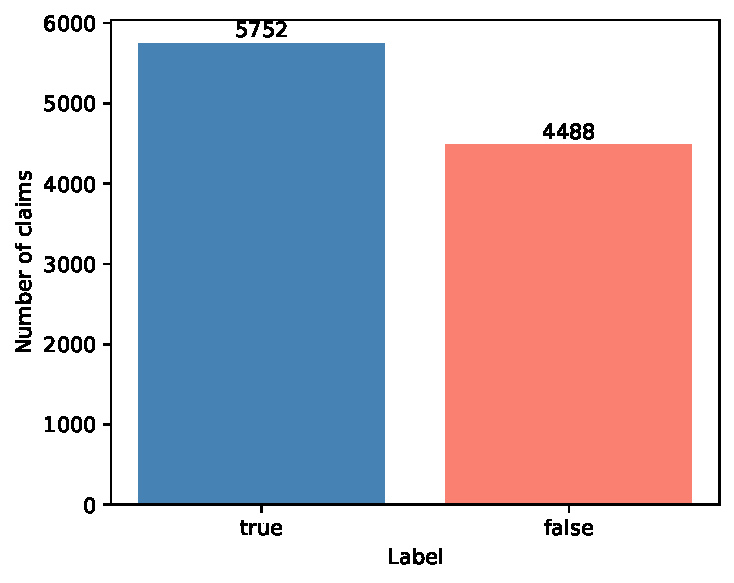
\includegraphics[width=0.7\textwidth]{Bilder/label_distribution_binary_train.pdf}
    \caption{Binary label distribution in the LIAR training set after mapping the 
    original six-class labels to true and false. The dataset exhibits a moderate 
    class imbalance, with true labels accounting for approximately 56\% of training 
    instances.}
    \label{fig:liar_label_distribution}
\end{figure}

\section{Task Definition}

This section defines the learning tasks addressed in this thesis and clarifies the modeling assumptions underlying the experimental setup. In particular, it distinguishes between binary and multi-class classification settings and introduces the notion of domain-aware versus domain-agnostic modeling, which plays a central role in the proposed agent-based framework.

\subsection{Binary vs. Multi-Class Classification}

Fake news and fact-checking tasks can be formulated in different ways depending on the target label space. Multi-class classification aims to predict fine-grained truthfulness labels, such as multiple degrees of factual correctness. While this formulation provides detailed output, it is also significantly more challenging due to class imbalance, annotation subjectivity, and limited training data for minority classes \cite{henning-etal-2023-survey}.

In this thesis, the task is formulated as a binary classification problem, where each claim is labeled as either true or false. This formulation aligns with many real-world fact-checking scenarios, where the primary objective is to distinguish factual from non-factual information \cite{vykopal2024generativelargelanguagemodels}. Binary classification also enables a more controlled evaluation of model behavior and facilitates fair comparison between different system configurations.

Rather than focusing on fine-grained truthfulness prediction, this thesis emphasizes the interaction between agents and domain information. Restricting the task to binary classification allows the analysis to concentrate on the impact of domain awareness and agent collaboration, without confounding effects introduced by highly imbalanced multi-class labels.

\subsection{Domain-Aware vs. Domain-Agnostic Settings}

Beyond the choice of label space, this thesis distinguishes between domain-aware and domain-agnostic modeling settings. In a domain-agnostic setting, the model receives only the claim text as input and must implicitly infer any relevant domain information during prediction. This reflects a standard classification setup commonly used in prior work \cite{schulhoff2025promptreportsystematicsurvey}.

In contrast, a domain-aware setting explicitly incorporates domain information into the decision process. In this thesis, domain knowledge is not derived from external sources, databases, or retrieval systems. Rather, it is operationalized exclusively through two mechanisms that rely on information already present in the LIAR dataset:

\begin{itemize}
    \item \textbf{Subject metadata as context:} The LIAR dataset provides 
    human-annotated subject tags for each statement (e.g., 
    \textit{health-care}, \textit{taxes}, \textit{elections}). These tags 
    are optionally prepended to the prompt as additional context, allowing 
    the model to leverage topical cues present in the dataset metadata.
    
    \item \textbf{Domain-specialized agents:} In the multi-agent framework, 
    claims are routed to domain-specific expert agents that have been 
    fine-tuned on domain-restricted subsets of the training data. These 
    agents implicitly encode domain knowledge through their training 
    distribution rather than through external information retrieval.
\end{itemize}

Consequently, domain awareness in this thesis refers to the structured use of existing dataset metadata and training signal. This design ensures full reproducibility and enables direct comparability with prior work on the same benchmark.

\section{Problem Setup Overview}

Figure~\ref{fig:pipeline_overview} illustrates the setup used in this thesis. Each input consists of a short political claim from the LIAR dataset, optionally accompanied by human-annotated subject tags. After preprocessing, the claim is passed to a 
classification system -- either a single LLM or a multi-agent pipeline -- which produces a binary verdict (\texttt{True} or 
\texttt{False}).

\begin{figure}[htbp]
\centering
\begin{tikzpicture}[
    box/.style={rectangle, rounded corners=3pt, draw, minimum width=4.5cm,
                minimum height=1.0cm, align=center, font=\small},
    data/.style={box, fill=orange!20, draw=orange!60},
    process/.style={box, fill=blue!15, draw=blue!50},
    optional/.style={box, fill=gray!15, draw=gray!50, dashed},
    output/.style={box, fill=green!20, draw=green!60},
    arrow/.style={-{Stealth}, thick},
]

\node[data] (dataset) at (0, 0) {
    \textbf{LIAR Dataset}\\
    \footnotesize short political claims};

\node[process] (preproc) at (0, -2) {
    \textbf{Preprocessing}\\
    \footnotesize text cleaning\\
    \footnotesize binary label mapping\\
    \footnotesize domain label mapping};

\node[optional] (subjects) at (5.5, -4) {
    \textbf{Subject Tags}\\
    \footnotesize (optional domain context)};

\node[process] (model) at (0, -4) {
    \textbf{Classification System}\\
    \footnotesize Single LLM or Multi-Agent};

\node[output] (verdict) at (0, -5.5) {
    \textbf{Binary Verdict}\\
    \footnotesize \texttt{True} / \texttt{False}};

\draw[arrow] (dataset) -- (preproc);
\draw[arrow] (preproc) -- (model);
\draw[arrow, dashed] (subjects) -- (model);
\draw[arrow] (model) -- (verdict);

\node[align=left, font=\footnotesize, text=gray] at (5.5, -0.0) {
    \textit{``The unemployment rate is}\\
    \textit{at a 50-year low.''}};

\draw[->, gray, dashed] (3.2, -0.0) -- (dataset.east);

\end{tikzpicture}
\caption{Overview of the binary claim verification setup. Each short political claim from the LIAR dataset is preprocessed and passed to a classification system, optionally augmented with human-annotated subject tags. The system outputs a binary verdict 
(\texttt{True}/\texttt{False}).}
\label{fig:pipeline_overview}
\end{figure}


  \chapter{Baseline Experiments with Single LLMs}
\label{chap:baseline_single}

This chapter establishes single-model baselines for binary claim verification on the LIAR benchmark. The experiments are organized 
along two main axes: (i) prompt-based evaluation, which tests how well off-the-shelf language models can classify political claims 
without task-specific training, and (ii) supervised fine-tuning, which quantifies the performance gains achievable through parameter-efficient adaptation.

The prompt-based block (Section~\ref{sec:prompt_baselines}) systematically varies output handling, subject conditioning, prompt 
design, reasoning strategies, and stylistic factors to identify which models and configurations provide the strongest starting 
point. The fine-tuning block (Section~\ref{sec:finetuning}) then investigates how much performance can be gained through LoRA 
adaptation under different training regimes and how well such adaptations transfer across domains.

Together, these experiments serve two purposes: they provide a quantitative reference for evaluating the multi-agent framework 
introduced in later chapters, and they identify the key limitations of single-model approaches -- output instability, domain 
overfitting, and limited generalization -- that motivate the agent-based design.

\section{Model Selection}

This section describes the selection of the Large Language Models used in this thesis. First, the criteria guiding the model selection are outlined. In the following, the chosen models are presented as representative examples of different Transformer architectures. The selected models form the basis for all subsequent experiments and comparisons.

\subsection{Selection Criteria}

To obtain a broad and meaningful selection of LLMs, models with different architectural designs were considered. The selection includes decoder-only, encoder-only, and encoder--decoder architectures, enabling an analysis of how architectural differences influence model behavior in the proposed setting. In addition, general-purpose foundation models were included, as they are commonly used across a wide range of NLP tasks.

Another important criterion was the public availability of the models. Only openly accessible models were selected to ensure reproducibility and transparency of the experimental setup. Furthermore, extremely large models were intentionally excluded. The goal of this thesis is not to achieve maximal performance through very large parameter counts, but rather to investigate how much performance can be obtained from relatively small to medium-sized models through effective prompting strategies and agent-based design.

In summary, the selected models
(i) represent different Transformer architectures,
(ii) are openly available,
(iii) have moderate model sizes, and
(iv) are widely used baseline or foundation models in current research.

\subsection{Representative LLMs}

Based on the criteria described above, the following models were selected as representative LLMs for the experiments:

\begin{itemize}
    \item LLaMA (Decoder-only)
    \item GPT-2 (Decoder-only)
    \item DeepSeek LLM (Decoder-only)
    \item T5 / FLAN-T5 (Encoder--Decoder)
    \item BERT (Encoder-only)
    \item Gemma (Decoder-only)
\end{itemize}

\paragraph{LLaMA}
LLaMA (Large Language Model Meta AI) is a decoder-only Transformer model that autoregressively predicts the next token in a sequence. It is based on self-attention, feed-forward networks, residual connections, and layer normalization. LLaMA was designed to achieve strong performance with relatively fewer parameters by training on large, high-quality text corpora. The original work demonstrates that LLaMA models can compete with significantly larger models despite their smaller size \cite{touvron2023llamaopenefficientfoundation}.

\paragraph{GPT-2}
GPT-2 is a decoder-only Transformer trained using a causal language modeling objective. Through masked self-attention, the model generates coherent and context-aware text without task-specific fine-tuning. Due to its simplicity, accessibility, and widespread use, GPT-2 serves as a strong baseline for generative language modeling tasks \cite{yenduri2023generativepretrainedtransformercomprehensive}.

\paragraph{DeepSeek LLM}
DeepSeek LLM is an open-source family of decoder-only Transformer models trained on very large-scale text data. In addition to pretraining, the models incorporate supervised fine-tuning and Direct Preference Optimization to enable conversational capabilities. Evaluations show that DeepSeek models perform strongly in domains such as code generation, mathematical reasoning, and logical problem solving \cite{deepseekai2024deepseekllmscalingopensource}.

\paragraph{T5 and FLAN-T5}
T5 (Text-to-Text Transfer Transformer) employs an encoder--decoder architecture and formulates all NLP tasks in a unified text-to-text format. This design allows the model to be applied flexibly to tasks such as classification, question answering, and summarization \cite{raffel2023exploringlimitstransferlearning}.  
FLAN-T5 extends T5 through instruction fine-tuning on a diverse set of tasks, significantly improving instruction-following ability and generalization across downstream applications \cite{chung2022scalinginstructionfinetunedlanguagemodels}.

\paragraph{BERT and RoBERTa}
BERT and RoBERTa are encoder-only Transformer models designed to learn rich bidirectional contextual representations. BERT is pretrained using masked language modeling and next sentence prediction objectives, enabling it to capture both left and right context effectively. RoBERTa builds upon BERT by optimizing the pretraining procedure, including training on larger text corpora, using dynamic masking, removing the next sentence prediction objective, and employing larger batch sizes. These improvements lead to stronger and more robust representations. Both models achieve strong performance across a wide range of natural language understanding tasks, particularly in text classification and inference, and are widely used as backbone models for downstream NLP applications \cite{devlin2019bertpretrainingdeepbidirectional, liu2019robertarobustlyoptimizedbert}.


\paragraph{Gemma}
Gemma is a family of lightweight, open language models developed by Google and based on a decoder-only Transformer architecture. The models incorporate modern architectural improvements such as rotary positional embeddings and multi-query attention. Despite their relatively small size, Gemma models achieve strong performance across a range of benchmarks while emphasizing efficiency and responsible deployment \cite{gemmateam2024gemmaopenmodelsbased}.

\subsection{Prompt Formatting Across Heterogeneous Language Models}

Since the selected language models differ not only in architecture but also in the format in which they expect textual input, prompt construction was implemented using a compatibility-oriented strategy. In the Hugging Face framework, some instruction-tuned or chat-oriented models provide a tokenizer-level chat template that converts structured conversational messages, such as system and user instructions, into the exact serialized prompt format expected by the respective model \cite{hf_chat_templates,hf_chat_templates_writing}. This mechanism is important because the prompt structure used at inference time should match the format a model has seen during instruction tuning or conversational post-training.

For this reason, prompts were not treated identically across all models. Instead, prompt construction followed a compatibility-oriented strategy. Whenever a model supported chat-style formatting, the prompt was rendered in a structured conversational form. Depending on the model, this could involve either separate conversational roles or a user-only chat prompt. If such formatting was not supported, the input was reduced to a plain text prompt. In later multi-agent experiments, this strategy was extended further by distinguishing between models that support an explicit system role and those that require system-level instructions to be embedded into the user message. In this way, all models could be evaluated within one unified framework while still respecting their model-specific input conventions.

This distinction was particularly relevant for the models used in this thesis. Meta's Llama 3.1 Instruct models explicitly support conversational prompt formatting with role-separated inputs, including a system instruction \cite{meta_llama_prompt}. In contrast, Google's instruction-tuned Gemma models do not support a separate system role and instead require such instructions to be embedded into the user message \cite{gemma_prompt_structure}. Base models such as DeepSeek-LLM-7B-Base, which are not primarily designed as chat models, are more appropriately addressed through plain text prompting when no dedicated chat template is provided \cite{deepseek_model_card}.

Overall, this prompting strategy should not be understood as a property of Transformer architecture itself, but rather as a practical compatibility layer between different model checkpoints and their expected input formatting. The approach ensures that each model is queried in a form that is as close as possible to its intended usage. This is consistent with the broader literature on instruction tuning, which shows that model behavior depends strongly on prompt phrasing, structure, and task formulation \cite{ouyang2022traininglanguagemodelsfollow,sanh2022multitaskpromptedtrainingenables,chung2022scalinginstructionfinetunedlanguagemodels}.

\section{Prompt-Based Baselines}
\label{sec:prompt_baselines}

This section establishes prompt-only baselines for binary factuality classification on the preprocessed LIAR test set (Section~\ref{sec:preprocessing}). To ensure comparability, the dataset, preprocessing, and evaluation metrics are held constant across runs. The baselines vary along three orthogonal axes: (1) output handling (Setup~A vs.\ Setup~B), (2) optional subject conditioning (domain-free vs.\ domain-informed), and (3) prompt design (basic vs.\ engineered prompts and structured inference variants introduced in later subsections). Complete results for all models and configurations are reported in Appendix~A Table~\ref{tab:zeroshot_setups} and Table~\ref{tab:appendix_all_baselines_full}.

The core baselines -- zero-shot evaluation and prompt engineering -- establish the performance ceiling for instruction-following without task-specific training. Beyond these, several exploratory extensions are evaluated: iterative prompting strategies, chain-of-thought reasoning, tone neutralization, and external domain classification. These extensions are not part of the primary baseline but provide additional insight into the factors that influence model behavior on the LIAR benchmark.

\subsection{Zero-Shot Evaluation Setups}
This subsection defines the two output-handling setups used throughout the prompt-based baselines. 
All runs use the same binary prompt, but differ in whether outputs are strictly parsed (Setup~A) or converted into a label via heuristic resolution (Setup~B).

\paragraph{Setup A: Strict parsing.}
Setup~A measures compliance with a strict output contract. A prediction is accepted only if the model output contains a single, unambiguous label token (\textit{True} or \textit{False}) in the expected format; otherwise the output is treated as \textit{unknown}. 
This setup is intentionally conservative and is designed to expose formatting failures and ambiguity in direct prompting. 
A known failure mode in strict parsing is that decoded outputs may include the prompt text itself; since the prompt contains the label words (\textit{true}, \textit{false}), naive extraction can accidentally match tokens originating from the prompt rather than from a clean model decision. 

\paragraph{Setup B: Forced decision with heuristic resolution.}
Setup~B enforces a binary decision for every instance. If the model output does not contain a clear \textit{True}/\textit{False} decision, a deterministic heuristic maps the response to one of the two labels. 
This setup therefore reflects the combined behavior of the model and a lightweight decision rule rather than purely unconstrained generation. 
However, it yields stable predictions for all inputs and enables clearer comparisons across models in settings where a deterministic label is required.

\subsubsection{Subject Conditioning (Domain-Informed Prompts)}

The LIAR dataset provides human-annotated subject tags for each statement -- comma-separated topical labels assigned by PolitiFact 
editors that describe the domain of the claim (e.g., \textit{``health-care, medicare''} or \textit{``taxes, federal-budget''}). These tags are not part of the statement text itself but constitute metadata that can optionally be used as domain context.

To test whether topical context helps zero-shot decisions, all experiments were performed in two prompt modes:

\begin{itemize}
    \item \textbf{Domain-free:} the prompt contains only the claim text.
    \item \textbf{Domain-informed:} LIAR subject labels are prepended to the prompt as additional context.
\end{itemize}

Subject conditioning is treated as an optional auxiliary input. No additional supervision is provided; the subject string is included only as prompt context. 

\paragraph{Results.}
Among the tested models, FLAN-T5-XL achieved the most balanced behavior in Setup A (without subjects), reaching an accuracy of 0.579. Encoder-only models showed mixed behavior under mask-based scoring: BERT-base reached 0.573 accuracy, while RoBERTa-large performed substantially lower (0.474).

Across the remaining decoder-only baselines, including GPT-J-6B, DeepSeek-LLM-7B-base, and the smaller Gemma-2B-IT model, behavior was largely identical to that of LLaMA-3.1-8B-Instruct. These models frequently failed to generate a clean, parsable binary answer under strict output constraints and effectively collapsed to near-constant predictions. As a result, they achieved similar accuracy values close to the majority-class baseline and exhibited very low macro-F1 scores, indicating limited discriminative ability in this strict zero-shot setting.

Under Setup B without subjects, the strongest overall performance was achieved by Gemma-7B-IT with an accuracy of 0.612. FLAN-T5-XL followed with 0.579, while BERT-base achieved 0.573. LLaMA-3.1-8B-Instruct reached 0.529 under the same conditions. In contrast, DeepSeek-LLM-7B-base showed strongly skewed predictions and obtained the lowest accuracy (0.436), indicating poor alignment with the binary prompting format in this configuration.

GPT-J-6B and Gemma-2B-IT benefited moderately from the forced-decision setup, achieving performance comparable to their larger counterparts, whereas DeepSeek-LLM-7B-base remained strongly biased toward a single class despite heuristic resolution.


\paragraph{Effect of subject information (domain-informed prompts).}
 Overall, adding subjects did not yield consistent improvements across models. For many models, results remained similar to the domain-free setting, suggesting that simply providing subject metadata is not sufficient to reliably steer zero-shot decisions. Notable exceptions were observed for LLaMA-3.1-8B-Instruct, which improved from 0.529 (Setup B, no subjects) to 0.568 (Setup B, with subjects). In contrast, Gemma-7B-IT showed a small decrease (from 0.612 to 0.608), and FLAN-T5-XL decreased from 0.579 to 0.571.

\paragraph{Summary.}
Across both setups, the experiments highlight two main findings. First, strict zero-shot evaluation is highly sensitive to output format and extraction decisions, and several models fail to produce reliably parsable binary outputs under minimal prompting. Second, forcing a binary decision (Setup~B) produces more stable and interpretable results and reveals model-specific differences, with Gemma-7B-IT and FLAN-T5-XL performing strongest among the evaluated baselines.

The key takeaway is that zero-shot prompting alone is insufficient for reliable binary claim verification on LIAR: even the strongest models reach only moderate accuracy (0.612), and performance is highly dependent on output handling and model architecture rather than on genuine factual reasoning ability. The performance gap between strict and forced-decision setups further suggests that many models lack robust instruction-following under minimal constraints. Overall, differences between decoder-only baselines (LLaMA, GPT-J, DeepSeek, Gemma) were small under strict zero-shot evaluation, whereas encoder–decoder models showed more stable behavior across setups.

For the multi-agent design, these findings have two concrete implications. First, the output instability observed under strict 
parsing motivates the use of structured output constraints (LM Format Enforcer) in the agent pipeline, ensuring that expert 
agents reliably produce machine-readable verdicts regardless of backbone-specific formatting behavior. Second, the model-specific 
performance differences -- particularly Gemma's stronger zero-shot alignment compared to LLaMA and DeepSeek -- inform the selection 
and configuration of backbone models for the domain-specialized expert agents in later chapters.

For readability, Table~\ref{tab:zeroshot_top2} summarizes the top-2 configurations per setup (A/B) and subject condition.

\begin{minipage}{\linewidth}
\centering
\captionof{table}{Top-2 zero-shot configurations on LIAR test ($n=1267$) for each setup 
(A/B) and subject condition. Ranking by Accuracy. Setup~A applies strict label 
parsing; Setup~B enforces a binary decision via heuristic resolution. 
Bal.\ Acc denotes balanced accuracy. TN/FP/FN/TP refer to the entries of the 
binary confusion matrix.}
\label{tab:zeroshot_top2}
\scriptsize
\begin{tabular}{ll l r r r r r r r r}
\toprule
Setup & Subjects & Model & n & Acc & Macro-F1 & Bal. Acc & TN & FP & FN & TP \\
\midrule
A (strict) & no  & flan-t5-xl        & 1267 & 0.579 & 0.571 & 0.570 & 280 & 273 & 261 & 453 \\
A (strict) & no  & bert-base-uncased & 1267 & 0.573 & 0.423 & 0.517 &  40 & 513 &  28 & 685 \\
\addlinespace
A (strict) & yes & flan-t5-xl        & 1267 & 0.571 & 0.570 & 0.574 & 334 & 219 & 325 & 389 \\
A (strict) & yes & bert-base-uncased & 1267 & 0.567 & 0.383 & 0.506 &  13 & 540 &   8 & 705 \\
\midrule
B (forced) & no  & gemma-7b-it       & 1267 & 0.612 & 0.583 & 0.588 & 222 & 331 & 161 & 553 \\
B (forced) & no  & flan-t5-xl        & 1267 & 0.579 & 0.571 & 0.570 & 280 & 273 & 261 & 453 \\
\addlinespace
B (forced) & yes & gemma-7b-it       & 1267 & 0.608 & 0.568 & 0.578 & 192 & 361 & 136 & 578 \\
B (forced) & yes & flan-t5-xl        & 1267 & 0.571 & 0.570 & 0.574 & 334 & 219 & 325 & 389 \\
\bottomrule
\end{tabular}
\end{minipage}

\subsection{Prompt Engineering Experiments}

To assess whether zero-shot performance can be improved through prompt design alone, a series of prompt engineering experiments was conducted. All experiments were performed on the preprocessed LIAR test set (Section~\ref{sec:preprocessing}) using a fixed set of prompt variants that differ in structure, instructional framing, and the use of contextual information.

Five prompt variants were evaluated:

\begin{itemize}
    \item \textbf{P0 (Basic Prompt):} A minimal binary question asking whether a statement is true or false.
    \item \textbf{P1 (Fake News, No Guessing):} Explicitly frames the task as factual verification and discourages guessing.
    \item \textbf{P2 (One-Shot Example):} Includes a simple example to illustrate the expected behavior.
    \item \textbf{P3 (Fact-Checking Assistant):} Assigns the model a specialized fact-checking role.
    \item \textbf{P4 (Subjects as Context Clues):} Explicitly instructs the model to use subject labels as contextual guidance.
\end{itemize}

Each prompt was evaluated in two modes: \emph{domain-free}, where only the claim text is provided, and \emph{domain-informed}, where subject labels are prepended to the prompt. Experiments were conducted for four representative models: LLaMA-3.1-8B-Instruct, Gemma-7B-IT, DeepSeek-LLM-7B, and FLAN-T5-XL. The exact prompt templates (P0--P4) are provided in Appendix~\ref{app:prompts}.


\subsubsection{Results and Analysis}

Overall, prompt engineering led to moderate but consistent performance differences, with improvements strongly dependent on the underlying model architecture.

Gemma-7B-IT achieved the strongest overall results across prompt variants. The best-performing configuration used the \emph{subjects-as-context-clues} prompt (P4) with subject information, reaching an accuracy of 0.615 and a macro-F1 score of 0.586. This indicates that Gemma is capable of leveraging explicit domain context when it is framed as auxiliary reasoning information rather than as raw metadata.

FLAN-T5-XL showed comparatively stable behavior across all prompt variants, with accuracies ranging between 0.57 and 0.60. While role-based and one-shot prompts produced slight improvements over the basic prompt, the overall gains were limited. This suggests that FLAN-T5-XL relies more heavily on its pretraining and instruction tuning than on prompt-level variations.

LLaMA-3.1-8B-Instruct benefited selectively from prompt engineering. Prompts that emphasized factual verification and discouraged guessing (P1) yielded improvements over the basic prompt, particularly when subject information was included. However, one-shot prompting and role-based instructions often led to performance degradation, indicating sensitivity to prompt structure and potential overfitting to superficial patterns.

In contrast, DeepSeek-LLM-7B performed poorly across nearly all prompt variants. Even with structured instructions and subject information, the model frequently collapsed to near-constant predictions, resulting in low macro-F1 scores. This suggests limited alignment with binary fact-checking tasks under zero-shot prompting.

Across all models, explicitly framing subject labels as contextual clues (P4) was more effective than simply prepending subject information. This finding highlights that domain information must be semantically integrated into the reasoning process in order to be useful.

\paragraph{Summary.}
The prompt engineering experiments demonstrate that carefully designed prompts can yield incremental performance improvements, particularly for instruction-following models such as Gemma-7B-IT. However, these gains remain limited, and no single prompt variant consistently resolves the shortcomings observed in strict zero-shot evaluation.

The key takeaway is that prompt design provides only marginal gains over the zero-shot baseline: the best prompt engineering configuration (Gemma-7B-IT, P4 with subjects, accuracy 0.615) barely exceeds the best zero-shot result (0.612), indicating a performance ceiling for prompt-only approaches on LIAR. Notably, domain information is only beneficial when semantically integrated into the reasoning process (P4) rather than simply prepended as raw metadata.

For the multi-agent design, these findings suggest two things. First, prompt design alone cannot compensate for the inherent difficulty of the task -- more structural changes such as domain specialization and agent collaboration are needed. Second, the P4 prompt strategy (subjects as context clues) proves most effective at integrating domain information and is therefore adopted as the default prompt template for domain-aware expert agents in the multi-agent pipeline.

For a compact overview, Table~\ref{tab:top2_promptengineering} reports the top configurations.

\begin{minipage}{\linewidth}
\centering
\captionof{table}{Top prompt-engineering configurations on LIAR test ($n=1267$), 
ranked by accuracy. One representative configuration per model is shown. 
Mean Conf denotes the mean predicted confidence for the positive class.}
\label{tab:top2_promptengineering}
\scriptsize
\begin{tabular}{l l l l r r r r r r r}
\toprule
Prompt & Model & Subjects & Acc & Macro-F1 & TN & FP & FN & TP & Mean Conf \\
\midrule
P4 (subjects as context clues) & gemma-7b-it           & yes & 0.615 & 0.586 & 223 & 330 & 158 & 556 & 0.913 \\
P1 (fake news, no guess)       & flan-t5-xl            & yes & 0.595 & 0.539 & 156 & 397 & 116 & 598 & 0.562 \\
P1 (fake news, no guess)       & Llama-3.1-8B-Instruct & yes & 0.579 & 0.579 & 362 & 191 & 343 & 371 & 0.757 \\
P2 (one-shot example)          & deepseek-llm-7b-base  & yes & 0.579 & 0.418 &  34 & 519 &  15 & 699 & 0.003 \\
\bottomrule
\end{tabular}
\end{minipage}

\subsection{Extended Prompt-Based Strategies}

Beyond the core zero-shot and prompt engineering baselines, four additional inference strategies were systematically evaluated to 
assess whether more sophisticated prompting mechanisms can overcome the limitations identified above: iterative prompting (self-consistency and reprompting), chain-of-thought reasoning, tone classification and neutralization, and external domain  classification. These strategies were motivated by prior work suggesting potential benefits for instruction-following models, 
but -- as the results show -- none of them produced consistent improvements over the simpler baselines on the LIAR benchmark. 
Their evaluation is therefore reported for completeness and to justify the transition to supervised fine-tuning and multi-agent 
approaches.

\subsubsection{Self-Consistency, Reprompting and Iterative self-refinement}

To further improve zero-shot performance beyond prompt wording alone, three iterative inference strategies were evaluated for the two strongest instruction-tuned decoder models from the previous experiments: LLaMA-3.1-8B-Instruct and Gemma-7B-IT. All methods were evaluated in a domain-free (\textit{no\_subjects}) and domain-informed (\textit{with\_subjects}) setting on the preprocessed LIAR test set.

\paragraph{Confidence-based label scoring.}
Instead of extracting labels from decoded text, both methods relied on likelihood-based scoring of the candidate answers \textit{True} and \textit{False}. For each input prompt, the model score was computed as the conditional log-likelihood of multiple surface forms of the labels (e.g., ``True'', `` true'', ``\textbackslash nTrue''). These scores were normalized into a two-class probability distribution, yielding $p(\text{True})$ and $p(\text{False})$, with confidence defined as $\max(p(\text{True}), p(\text{False}))$. This approach avoids the parsing issues observed in strict decoding-based evaluation and allows a consistent confidence estimate for downstream decision rules.

\paragraph{Self-consistency.}
Self-consistency aggregates predictions across multiple prompt paraphrases for the same claim. For each instance, $N=5$ prompt variants were generated using lightweight paraphrasing templates, and the final prediction was derived via a weighted vote based on the model's two-class probabilities. This method aims to reduce variance from prompt sensitivity and stabilize decisions through ensembling.

For Gemma-7B-IT, self-consistency achieved an accuracy of 0.609 without subjects and 0.603 with subjects. For LLaMA-3.1-8B-Instruct, self-consistency yielded smaller gains, reaching 0.538 accuracy without subjects and 0.541 with subjects. Overall, self-consistency improved stability compared to the basic baseline for both models, but the gains were modest and dependent on model behavior.

\paragraph{Reprompting.}
Reprompting applies staged prompting based on confidence. Each claim was first evaluated using the base prompt. If the confidence score exceeded a fixed threshold ($\tau = 0.75$), the prediction was accepted. Otherwise, a second-stage prompt was applied that explicitly encouraged the model to reconsider the claim with a more structured instruction (including a subject-aware variant when enabled).

Reprompting produced the strongest results among the tested strategies for Gemma-7B-IT, achieving 0.614 accuracy without subjects and 0.616 with subjects. This indicates that Gemma benefits from conditional escalation when uncertain, while still producing reliable high-confidence predictions for many instances. In contrast, reprompting did not benefit LLaMA: accuracy decreased to 0.502 without subjects and 0.526 with subjects, suggesting that the second-stage prompt tended to amplify existing biases rather than correcting uncertain cases.

\paragraph{Iterative self-refinement.}
As an additional baseline, iterative self-refinement was evaluated for both Gemma-7B-IT and LLaMA-3.1-8B-Instruct, in which the model is prompted to critique and revise its own prediction over multiple rounds. For Gemma, this method collapsed to near-constant \texttt{True} predictions (TN$\approx$2, TP$\approx$713) with extremely low confidence scores (Mean Conf$\approx 2.85 \times 10^{-7}$). LLaMA showed less severe collapse but similarly low confidence ($5.4 \times 10^{-4}$) and reduced accuracy (0.519), indicating that iterative revision destabilized decision behavior for both models rather than improving it.

\paragraph{Summary.}
Overall, the evaluated strategies highlight that iterative prompting can improve performance for some models, but not universally. Gemma-7B-IT benefited from reprompting and achieved the best overall results in this block of experiments (accuracy 0.616), while LLaMA-3.1-8B-Instruct showed limited improvements under self-consistency (0.541) and degraded under reprompting (0.526). Iterative 
self-refinement collapsed to near-constant \texttt{True} predictions for both models, with extremely low confidence scores, indicating that the iterative revision process destabilized decision behavior rather than improving it. These observations motivate the use of more structured coordination and verification mechanisms, which are later explored in the multi-agent setting. For a compact overview, Table~\ref{tab:top_iterative} reports the top configurations for each method and model.

\begin{minipage}{\linewidth}
\centering
\captionof{table}{Top configurations per method and model on LIAR test ($n=1267$), 
ranked by accuracy within each method group. Mean Conf denotes the mean predicted confidence for the positive class.}
\label{tab:top_iterative}
\scriptsize
\begin{tabular}{l l l l r r r r r r r}
\toprule
Method & Model & Subjects & Acc & Macro-F1 & TN & FP & FN & TP & Mean Conf \\
\midrule
reprompting               & gemma-7b-it           & yes & 0.616 & 0.584 & 213 & 340 & 146 & 568 & 0.979 \\
self-consistency          & gemma-7b-it           & no  & 0.609 & 0.584 & 231 & 322 & 174 & 540 & 0.933 \\
self-consistency          & Llama-3.1-8B-Instruct & yes & 0.541 & 0.529 & 442 & 111 & 471 & 243 & 0.905 \\
reprompting               & Llama-3.1-8B-Instruct & yes & 0.526 & 0.510 & 451 & 102 & 498 & 216 & 0.882 \\
iterative self-refinement & gemma-7b-it           & no  & 0.564 & 0.364 &   2 & 551 &   1 & 713 & 2.85e-07 \\
iterative self-refinement & Llama-3.1-8B-Instruct & yes & 0.519 & 0.499 & 456 &  97 & 512 & 202 & 5.4e-04 \\
\bottomrule
\end{tabular}
\end{minipage}

\subsubsection{Chain-of-Thought Prompting}

To test whether explicitly eliciting intermediate reasoning improves factuality judgments, a chain-of-thought (CoT) prompting setup was evaluated for LLaMA-3.1-8B-Instruct and Gemma-7B-IT. The prompt required the model to (i) provide a short justification (1--3 sentences) based on publicly verifiable facts and (ii) output a final decision in a fixed format (\texttt{Final answer: True/False}). Experiments were run in a domain-free condition (statement only) and a domain-informed condition (subjects prepended).

Predictions were extracted using a forced True/False parser (Setup-B-like), while confidence was computed at the decision point by scoring the next-token probability distribution after the marker \texttt{Final answer:}. This yields a confidence estimate conditioned on the generated reasoning rather than on the raw prompt alone.

\paragraph{Results.}
CoT prompting improved performance for Gemma-7B-IT relative to the basic baseline. Gemma achieved 0.604 accuracy in both modes (0.601 macro-F1 without subjects; 0.597 macro-F1 with subjects), indicating that the model benefited from producing an explicit justification but did not consistently leverage subject metadata in this configuration. The mean confidence at the decision point was very high (approximately 0.99), suggesting that the format strongly constrains the output distribution.

In contrast, CoT prompting did not benefit LLaMA-3.1-8B-Instruct. Accuracy remained low at 0.492 without subjects and increased only marginally to 0.506 with subjects (macro-F1: 0.449 and 0.476, respectively). This suggests that for LLaMA in this setup, generating short reasoning did not translate into more accurate binary decisions, even though confidence values were also high (around 0.93--0.94).

\paragraph{Summary.}
Overall, CoT prompting helped the better-aligned instruction model (Gemma-7B-IT) but did not reliably improve factual classification for LLaMA-3.1-8B-Instruct. These results support the broader observation that reasoning prompts can yield gains, but their effectiveness is model-dependent and does not by itself resolve the limitations of zero-shot factual verification on LIAR. For a compact overview, Table~\ref{tab:top_cot} reports the top configurations.

\begin{minipage}{\linewidth}
\centering
\captionof{table}{Chain-of-Thought configurations on LIAR test ($n=1267$), ranked 
by accuracy. Results are shown for both subject conditions per model. Mean Conf 
denotes the mean predicted confidence at the \texttt{Final answer:} decision point.}
\label{tab:top_cot}
\scriptsize
\begin{tabular}{l l l l r r r r r r r}
\toprule
Method & Model & Subjects & Acc & Macro-F1 & TN & FP & FN & TP & Mean Conf \\
\midrule
chain-of-thought & gemma-7b-it           & no  & 0.604 & 0.601 & 331 & 222 & 280 & 434 & 0.987 \\
chain-of-thought & gemma-7b-it           & yes & 0.604 & 0.597 & 298 & 255 & 247 & 467 & 0.991 \\
chain-of-thought & Llama-3.1-8B-Instruct & yes & 0.506 & 0.476 & 473 &  80 & 546 & 168 & 0.93  \\
chain-of-thought & Llama-3.1-8B-Instruct & no  & 0.492 & 0.449 & 487 &  66 & 578 & 136 & 0.933 \\
\bottomrule
\end{tabular}
\end{minipage}

\subsubsection{Tone Classification and Neutralization}

To investigate whether stylistic factors influence factuality judgments, an additional pipeline was implemented that (i) classifies the tone of each statement and (ii) rewrites it into a neutral, objective formulation. Tone was predicted using the labels \{\textit{neutral}, \textit{subjective}, \textit{ironic}, \textit{emotional}\} via an instruction prompt. Neutralization then rewrote each statement to remove sarcasm, exaggeration, and emotionally loaded phrasing while preserving meaning and without adding new facts. Both steps were performed with an instruction-tuned decoder model, and the resulting tone labels and neutralized statements were stored for downstream evaluation.

Using these artifacts, two base prompts (P0 and P4) were reevaluated under four conditions: (1) original statement, (2) neutralized statement, (3) original statement with an explicit tone line (\texttt{Tone: <label>}), and (4) neutralized statement with an explicit tone line. Each condition was tested with and without subject metadata.

\paragraph{Results: Gemma-7B-IT.}
For Gemma, adding tone information to the \emph{original} statement slightly improved accuracy in the best configurations. The strongest result was obtained with P0 in the subject-informed setting when tone was included (orig\_plus\_tone), reaching 0.616 accuracy. With P4 and tone, accuracy remained similarly high (0.615 with subjects; 0.613 without subjects) and macro-F1 improved in some configurations (e.g., 0.597 for P4 with subjects). In contrast, neutralization consistently reduced performance across prompts: accuracies dropped to approximately 0.565--0.579 depending on configuration, indicating that removing expressive or stylistic cues harmed the model's ability to match the dataset labels.

\paragraph{Results: LLaMA-3.1-8B-Instruct.}
For LLaMA, the tone/neutralization interventions did not produce consistent gains. The best LLaMA configuration in this block was obtained under neutral\_plus\_tone with P0 and subjects (0.522 accuracy), but most settings remained close to chance-level and often below earlier subject-informed baselines. Notably, adding subjects tended to help LLaMA in several conditions compared to no-subjects, but the overall absolute performance stayed limited.

\paragraph{Summary.}
These results suggest that label-relevant stylistic signals are present in LIAR: rewriting statements into a strictly neutral style reduces accuracy, especially for Gemma. Conversely, explicitly exposing the tone label can provide a small benefit for some prompt/model combinations, but the effect is modest and not robust across architectures. For a compact overview, Table~\ref{tab:top_tone} reports the top configurations.

\begin{minipage}{\linewidth}
\centering
\captionof{table}{Top configurations for tone classification and neutralization on 
LIAR test ($n=1267$), ranked by accuracy. Top-2 configurations per model are shown.}
\label{tab:top_tone}
\scriptsize
\begin{tabular}{l l l l r r r r r r}
\toprule
Method & Model & Subjects & Acc & Macro-F1 & TN & FP & FN & TP \\
\midrule
P0 + orig\_plus\_tone    & gemma-7b-it           & yes & 0.616 & 0.574 & 190 & 363 & 123 & 591 \\
P4 + orig\_plus\_tone    & gemma-7b-it           & yes & 0.615 & 0.597 & 258 & 295 & 193 & 521 \\
P0 + neutral\_plus\_tone & Llama-3.1-8B-Instruct & yes & 0.522 & 0.522 & 335 & 218 & 388 & 326 \\
P0 + neutral\_plus\_tone & Llama-3.1-8B-Instruct & no  & 0.511 & 0.511 & 321 & 232 & 387 & 327 \\
\bottomrule
\end{tabular}
\end{minipage}

\subsubsection{External Domain Classification}

Beyond the human-provided LIAR subject labels, an external domain classifier was used to generate a single coarse-grained domain label for each statement. A zero-shot natural language inference model (BART-large-MNLI) was applied with a fixed list of candidate domains (e.g., \textit{health}, \textit{economy}, \textit{politics}, \textit{law}, \textit{crime}, etc.), and the top-1 predicted domain label was stored alongside the dataset.

To measure whether externally inferred domain context can replace or complement the original subject metadata, the fact-checking prompts (P0 and P4) were evaluated under three subject modes: (i) no subjects, (ii) human LIAR subjects, and (iii) external top-1 domain label. All runs used likelihood-based next-token scoring for \textit{True}/\textit{False} (Setup-B-like), ensuring consistent evaluation across conditions.

\paragraph{Results.}
For Gemma-7B-IT, using human subjects produced the best results (P0: 0.612 accuracy; P4: 0.610). Replacing human subjects with the external top-1 domain led to a small performance drop (P0: 0.608; P4: 0.602), but still outperformed the no-subjects condition in some cases. This indicates that externally inferred domain context can provide useful coarse guidance, but does not fully substitute for the richer human subject annotations.

For LLaMA-3.1-8B-Instruct, none of the subject modes produced strong performance. The best LLaMA result in this comparison was obtained using P4 without subjects (0.492 accuracy). Human subjects increased P0 accuracy relative to the no-subjects baseline (0.481 vs. 0.455), but external domains did not improve over human subjects and remained below 0.472 in the reported configurations. Overall, subject/domain conditioning provided only limited benefit for LLaMA under this evaluation scheme.

\paragraph{Summary.}
External domain classification yields a scalable form of contextual metadata that can partially recover the benefit of human subject labels for Gemma-7B-IT, but it does not consistently improve results for LLaMA-3.1-8B-Instruct. Taken together with the previous experiments, these findings reinforce that contextual information is only effective when the underlying model is capable of integrating it reliably, motivating more structured approaches in later sections. For a compact overview, Table~\ref{tab:top_extdomain} reports the top configurations for each baseline block.

\begin{minipage}{\linewidth}
\centering
\captionof{table}{Comparison of subject conditions for external domain classification 
on LIAR test ($n=1267$), ranked by accuracy. Results show the best prompt per 
subject condition and model.}
\label{tab:top_extdomain}
\scriptsize
\begin{tabular}{l l l r r r r r r}
\toprule
Method & Model & Subjects & Acc & Macro-F1 & TN & FP & FN & TP \\
\midrule
P0 + human subjects    & gemma-7b-it           & yes & 0.612 & 0.590 & 243 & 310 & 182 & 532 \\
P0 + ext\_domain\_top1 & gemma-7b-it           & yes & 0.608 & 0.586 & 239 & 314 & 183 & 531 \\
P0 + no subjects       & gemma-7b-it           & no  & 0.606 & 0.591 & 263 & 290 & 209 & 505 \\
\addlinespace
P4 + no subjects       & Llama-3.1-8B-Instruct & no  & 0.492 & 0.450 & 486 &  67 & 577 & 137 \\
P0 + human subjects    & Llama-3.1-8B-Instruct & yes & 0.481 & 0.416 & 517 &  36 & 621 &  93 \\
P0 + ext\_domain\_top1 & Llama-3.1-8B-Instruct & yes & 0.471 & 0.398 & 520 &  33 & 637 &  77 \\
\bottomrule
\end{tabular}
\end{minipage}

\paragraph{Overall summary of extended strategies.}

Across all four extended strategies, none produced consistent improvements over the core prompt-based baselines on the LIAR benchmark. Self-consistency and reprompting yielded modest gains for Gemma-7B-IT but were ineffective or harmful for LLaMA-3.1-8B-Instruct. Chain-of-thought reasoning helped Gemma but not LLaMA, suggesting that reasoning prompts are model-dependent. Tone neutralization consistently reduced performance, indicating that stylistic signals in LIAR are label-relevant rather than noise. External domain classification partially recovered the benefit of human subject labels but did not surpass them.

The key takeaway is that no prompt-level intervention -- regardless of its sophistication -- reliably overcomes the fundamental difficulty of binary claim verification on LIAR. Performance gains are marginal, model-dependent, and do not generalize across architectures.

For the multi-agent design, these findings have one concrete implication: prompt engineering alone is insufficient and supervised adaptation is necessary. The transition to fine-tuning in the next section is therefore not merely a design choice but 
a direct consequence of the prompt-based ceiling observed here.

\section{Fine-Tuning Experiments}
\label{sec:finetuning}

The zero-shot and prompt-based baselines in the previous section showed two recurring limitations: (i) several models struggled to produce stable and discriminative binary decisions under minimal prompting, and (ii) even under forced-decision decoding, performance gains from prompt engineering remained modest and model-dependent. To move beyond purely inference-time steering, the next set of experiments applies supervised adaptation via parameter-efficient fine-tuning. The goal is not to maximize absolute benchmark performance, but to quantify how much factuality classification performance can be obtained from moderately sized open models when trained directly on the task, and how well such adaptations transfer across domains.

\subsection{Fine-Tuning Method: LoRA Adapters}

All fine-tuning experiments were performed using Low-Rank Adaptation (LoRA), a parameter-efficient method that injects trainable low-rank matrices into selected linear projections while keeping the original backbone weights frozen. In practice, this reduces GPU memory requirements and training time compared to full fine-tuning, while still allowing the model to learn task-specific decision boundaries. Following common practice for decoder-only Transformers, LoRA modules were applied to the attention projections (typically \texttt{q\_proj}, \texttt{k\_proj}, \texttt{v\_proj}, \texttt{o\_proj}). The LoRA configuration was kept fixed across runs to enable consistent comparisons:
\begin{itemize}
    \item rank $r=8$,
    \item $\alpha=32$,
    \item dropout $0.05$,
    \item bias: none.
\end{itemize}
During training, gradient checkpointing was enabled and caching was disabled (\texttt{use\_cache=False}) to reduce memory usage and stabilize training for long sequences.

\subsection{Training Data and Regimes}

Fine-tuning was conducted under four training regimes, each corresponding to one dataset condition used throughout the evaluation:

\begin{itemize}
    \item \textbf{General (LIAR)}: training on the full LIAR training split (binary labels).
    \item \textbf{Healthcare}: training on the healthcare subset (domain-specific).
    \item \textbf{Taxes}: training on the taxes subset (domain-specific).
    \item \textbf{Synthetic}: training on synthetically generated fact-checking instances (ChatGPT).
\end{itemize}

For each regime, two prompt settings were evaluated:
(i) \emph{no\_subjects} (statement only) and
(ii) \emph{with\_subjects} (LIAR subject metadata prepended).
This yields a controlled comparison of whether additional topical context improves learning and/or generalization beyond what the model can infer from the statement alone.

\paragraph{Dataset preprocessing and domain subset construction.}
All datasets used for fine-tuning were preprocessed using the pipeline described in Section~\ref{sec:preprocessing}. 
For domain-specific fine-tuning, the two largest LIAR subject categories were selected (healthcare and taxes). 
Domain subsets were constructed by retaining statements whose subject list contained the target domain and at most one additional subject label. 
This constraint reduces topic ambiguity while preserving a realistic multi-label setting. 
When enabled, subject information was provided only as additional input context in the prompt, not as a separate supervision signal.

\subsection{Training Setup and Hyperparameters}

All runs used the same training pipeline and hyperparameters to make results comparable across models and datasets. Inputs were formatted using the same binary fact-checking prompt template used in the prompt baselines, and for instruction-tuned chat models the tokenizer's chat template was applied where available. Training was performed in a \emph{completion-only} style: the model receives the prompt and is trained to generate exactly one of the two labels (\texttt{True} or \texttt{False}), while prompt tokens are masked out in the loss.

Key hyperparameters were:
\begin{itemize}
    \item max sequence length: 512 tokens,
    \item epochs: 3,
    \item learning rate: $2 \cdot 10^{-5}$,
    \item per-device batch size: 2,
    \item gradient accumulation: 4 (effective batch size 8),
    \item optimizer: AdamW (\texttt{adamw\_torch}),
    \item mixed precision: bfloat16 (\texttt{bf16=True}),
    \item validation split: 5\% (random split with fixed seed),
    \item training objective: completion-only (prompt tokens masked, loss computed only on the label ``True''/``False''),
    \item prompt template: \texttt{standard} (two variants: without subjects and with subjects, see below).
\end{itemize}

\noindent Prompt without subjects:
\begin{verbatim}
Statement: {statement}
Task: Verify the factual accuracy of the statement using only publicly available and objective information. Do not guess.
Answer with only one word: True or False.
Answer:
\end{verbatim}

\noindent Prompt with subjects:
\begin{verbatim}
Subjects: {subjects}
Statement: {statement}
Task: Verify the factual accuracy of the statement using only publicly available and objective information.
Use the subjects only as context clues; they may be incomplete. Do not guess.
Answer with only one word: True or False.
Answer:
\end{verbatim}

Evaluation during training was performed at fixed step intervals. For runs trained on the full LIAR training set, validation was executed every 250 optimization steps; for the smaller domain-specific datasets, validation was executed every 10 steps. Checkpoints were saved using the same interval.

To avoid losing the best-performing model state when training continues beyond the validation optimum, the checkpoint with the lowest validation loss was tracked and retained. After training, this best checkpoint was additionally exported into a dedicated directory (e.g., \texttt{best\_adapter}). Consequently, all downstream evaluations consistently use the strongest model state observed during training rather than the final checkpoint.


\subsection{Evaluation Protocol and Metrics}

After training, each adapter was evaluated on multiple test sets to measure both \emph{in-domain performance} and \emph{cross-domain transfer}. Specifically, models trained on each regime (general, healthcare, taxes, synthetic) were evaluated on:
\begin{itemize}
    \item the LIAR test set (generalization to the main benchmark),
    \item the healthcare test subset,
    \item the taxes test subset,
    \item the synthetic test set.
\end{itemize}

Predictions were obtained deterministically, and the reported metrics include accuracy, macro-F1, positive-class precision/recall, the confusion matrix, and confidence statistics (mean confidence overall and separated by correct/incorrect predictions). This provides a more complete picture than accuracy alone, especially in cases where models become biased toward one class (which can produce deceptively acceptable accuracy but very low macro-F1).

\subsection{Fine-Tuning Results}

The fine-tuning results reveal three consistent patterns across models and training regimes. Complete results for all train/eval combinations, models, and subject settings are reported in Appendix~D Table~\ref{tab:finetune_all_results}. For readability, Table~\ref{tab:finetune_bestof} summarizes the best-performing configurations per training regime and evaluation target.

\paragraph{(1) General training yields the strongest LIAR performance.}
Adapters trained on the general LIAR data achieve the best results when evaluated on the LIAR test set. Among the three decoder-only models tested (Gemma-7B-IT, LLaMA-3.1-8B-Instruct, DeepSeek-LLM-7B-base), LIAR-trained adapters without subjects perform best overall, with LLaMA and DeepSeek slightly ahead of Gemma in this setting. This indicates that direct supervision on the target distribution is more impactful than prompt engineering alone, and that the task is learnable with relatively small parameter-efficient updates.

\paragraph{(2) Domain-specific fine-tuning improves in-domain results but transfers poorly.}
Training on healthcare or taxes improves performance on the corresponding domain test set, but this specialization does not reliably transfer to the general LIAR benchmark. In cross-domain evaluation, domain-trained adapters typically perform 
worse than general-trained adapters on LIAR, consistent with domain overfitting: the adapter learns patterns and priors that are useful within the narrow domain but do not generalize to broader political and public-figure claims that dominate LIAR. Notably, cross-domain transfer is asymmetric: healthcare-trained adapters transfer more reliably to taxes (0.667) than taxes-trained dapters transfer to healthcare (0.639), suggesting that the healthcare domain provides a broader and more generalizable training signal.

\paragraph{(3) Synthetic training shows a strong distribution mismatch.}
Synthetic-trained adapters reach high performance on the synthetic test set, but their LIAR performance drops substantially compared to adapters trained on LIAR. This suggests that the synthetic data captures a different distribution of linguistic cues and label correlations than LIAR, and that high synthetic accuracy does not necessarily indicate robust factual reasoning on real-world claims.

\paragraph{Effect of subjects (context metadata).}
Across regimes, subject metadata does not yield a uniform benefit. In some in-domain cases, subjects help by providing a coarse topical prior, but in cross-domain settings they can hurt or lead to unstable precision/recall trade-offs, suggesting shortcut learning: the model may over-rely on topic-label correlations rather than statement-level evidence. Overall, subjects appear most beneficial when the underlying model is already well-aligned to the task and capable of integrating auxiliary context, whereas weaker or less-stable configurations do not consistently benefit.

\paragraph{Summary.}
In contrast to the zero-shot baseline results, supervised adaptation via LoRA produces stable and discriminative classifiers. However, the experiments also show that fine-tuning can trade off generalization for specialization: domain-specific adapters can improve in-domain accuracy but often reduce performance on the main benchmark. Finally, synthetic supervision appears insufficient to replace real benchmark data, reinforcing the importance of training on distributions that match the target evaluation setting.

The key takeaway is that fine-tuning substantially improves over prompt-only approaches but introduces new limitations: domain 
overfitting reduces cross-domain robustness, and all models still rely on dataset-specific patterns rather than genuine fact verification. The best single-model result (LLaMA-3.1-8B-Instruct, LIAR-trained, accuracy 0.667) establishes the performance ceiling for single-model approaches and serves as the primary reference point for evaluating the multi-agent framework.

For the multi-agent design, the fine-tuning results have three concrete implications. First, LLaMA-3.1-8B-Instruct consistently 
outperforms Gemma and DeepSeek in terms of balanced class behavior and cross-domain stability, making it the preferred backbone for 
domain-specialized expert agents. Second, domain-specific fine-tuning is feasible and improves in-domain performance, motivating the use of domain-restricted training subsets for individual expert agents in the multi-agent pipeline. Third, the observed domain overfitting motivates the routing-based design in the final framework, where claims are directed to the most relevant expert rather than evaluated by all experts indiscriminately.

\begin{table}[!htbp]
\centering
\scriptsize
\setlength{\tabcolsep}{3.5pt}
\renewcommand{\arraystretch}{1.08}
\caption{Best fine-tuned configuration per training regime and evaluation target (selected by Accuracy; tie-breaker: Macro-F1). Full fine-tuning results are provided in Appendix~C (Table~\ref{tab:finetune_all_results}).}
\label{tab:finetune_bestof}
\begin{tabular}{l l l c r r r r r}
\toprule
Train set & Eval set & Best model & Subjects & Acc & Macro-F1 & Prec(+) & Rec(+) & Mean Conf \\
\midrule
General (LIAR) & LIAR test      & Llama-3.1-8B-Instruct & yes & 0.667 & 0.649 & 0.674 & 0.793 & 0.731 \\
General (LIAR) & Synthetic test & deepseek-llm-7b-base  &  no & 0.823 & 0.822 & 0.785 & 0.832 & 0.680 \\
\addlinespace
Healthcare     & Healthcare test & Llama-3.1-8B-Instruct &  no & 0.711 & 0.711 & 0.725 & 0.690 & 0.701 \\
Healthcare     & LIAR test       & Llama-3.1-8B-Instruct &  no & 0.650 & 0.642 & 0.683 & 0.704 & 0.685 \\
Healthcare     & Taxes test      & Llama-3.1-8B-Instruct & yes & 0.667 & 0.661 & 0.615 & 0.828 & 0.681 \\
\addlinespace
Taxes          & Taxes test      & gemma-7b-it           & yes & 0.650 & 0.642 & 0.682 & 0.517 & 0.841 \\
Taxes          & LIAR test       & Llama-3.1-8B-Instruct & yes & 0.609 & 0.597 & 0.642 & 0.689 & 0.774 \\
Taxes          & Healthcare test & gemma-7b-it           &  no & 0.639 & 0.629 & 0.714 & 0.476 & 0.881 \\
\addlinespace
Synthetic      & Synthetic test  & gemma-7b-it           & yes & 0.885 & 0.884 & 0.871 & 0.871 & 0.928 \\
Synthetic      & LIAR test       & gemma-7b-it           & yes & 0.604 & 0.604 & 0.690 & 0.539 & 0.834 \\
\bottomrule
\end{tabular}
\end{table}

\section{Results and Analysis}

This section consolidates the empirical findings from the single-model experiments. Since the preceding sections already reported results close to each experimental setup, the goal here is to extract overarching patterns, relate them across regimes (zero-shot vs.\ fine-tuning), and highlight implications for later multi-agent experiments.

\subsection{Performance Overview Across Baselines and Fine-Tuning}

Across all single-model experiments, supervised adaptation via LoRA leads to the largest and most reliable performance gains compared to purely prompt-based steering. In the zero-shot and prompt engineering blocks, results were highly sensitive to output format and label extraction, and several decoder-only models exhibited degenerate behavior under strict parsing (Setup~A). Even under forced decision making (Setup~B), prompt engineering yielded only modest and model-dependent improvements.

Fine-tuning reduces these instabilities substantially: the model is trained to produce a short, consistent continuation (\texttt{True}/\texttt{False}) and therefore behaves more like a standard discriminative classifier. On the main benchmark (LIAR test), LIAR-trained adapters outperform the strongest prompt-based baselines, indicating that the task-relevant decision boundary is learnable with relatively small parameter-efficient updates. However, the absolute performance remains moderate, suggesting that the model still relies on dataset-specific cues rather than robust external fact verification.

\subsection{In-Domain Performance vs.\ Cross-Domain Transfer}

A central result of the fine-tuning experiments is the trade-off between \emph{specialization} and \emph{generalization}. Models trained on the full LIAR training set achieve the strongest performance on the LIAR test set. In contrast, adapters trained on domain-specific subsets (healthcare or taxes) show improved in-domain behavior but transfer less reliably to LIAR. This pattern is consistent with domain overfitting: when training data is narrow, the adapter can learn strong domain priors (e.g, typical wording, recurring entities, or claim style) that help within the domain but do not generalize to the broader claim distribution in LIAR.

The synthetic regime further highlights distribution mismatch. Synthetic-trained adapters reach very high performance on synthetic test data, but their performance on LIAR drops substantially. This indicates that synthetic claims capture different linguistic regularities and label correlations than LIAR. In other words, strong in-domain synthetic accuracy is not evidence of robust factual reasoning on real-world benchmark statements.

\subsection{Effect of Subject Metadata}

Subject labels (domain metadata) do not provide a consistent improvement across models and regimes. In the zero-shot baselines, subjects sometimes helped (e.g., for LLaMA) but often had no effect or caused small drops (e.g., for Gemma under some settings). After fine-tuning, the effect remains mixed: subjects can act as a useful topical prior in-domain, but can also encourage shortcut learning if the model over-relies on topic--label correlations rather than claim content.

This is also reflected in shifts of precision/recall trade-offs. In several configurations, adding subjects increases true negatives while increasing false negatives (or vice versa), indicating that the model changes its decision threshold or class bias depending on whether topic information is present. Overall, subject metadata is beneficial only when the underlying model can integrate it in a calibrated way. Otherwise, it can introduce additional spurious signals that reduce transfer performance.

\subsection{Error Patterns and Confusion Matrix Dynamics}

Beyond accuracy, macro-F1 and confusion matrices reveal recurring error modes. For multiple LIAR-evaluated runs, models tend to show strong positive-class recall but comparatively weaker specificity, leading to many false positives. This pattern suggests that the model often defaults toward predicting one label under uncertainty (depending on training regime and prompt setting). Such imbalances are not always visible from accuracy alone, especially if the dataset is not perfectly balanced or if the majority-class baseline is non-trivial. An exception to the typical True-class bias is observed for the Taxes-trained Gemma adapter, which shows comparatively low recall for the positive class (Rec(+) = 0.517), suggesting that the narrow tax-domain training distribution induces a different label prior than the broader LIAR or Healthcare regimes.

Domain-specific adapters show analogous patterns: performance gains on small domain test sets can be driven by learning a narrow set of lexical and stylistic cues that correlate with labels in that domain. When evaluated outside that domain, these cues no longer hold, producing a measurable increase in misclassification and a drop in macro-F1.

\subsection{Interpretation: Benefits of Fine-Tuning}

The results support two complementary interpretations:

\paragraph{Fine-tuning improves format reliability and task alignment.}
LoRA adaptation turns the problem into a supervised decision task with stable output behavior. This largely removes the parsing failure modes observed in strict zero-shot prompting and yields consistent, reproducible predictions.

\paragraph{Fine-tuning does not guarantee real fact checking.}
Even after fine-tuning, the models still do not use external sources or retrieval. They are trained only to match the dataset labels. Therefore, higher scores may come from learning correlations in the data (e.g., writing style cues, topic biases, or annotation artifacts) rather than truly verifying a claim against evidence. The weak cross-domain transfer—especially for adapters trained on synthetic data—supports this: when the data distribution changes, performance drops, which suggests that the models rely on dataset-specific shortcuts instead of robust fact verification.

\subsection{Implications for Multi-Agent Fact-Checking}

Taken together, the single-model results motivate stronger mechanisms than single-pass prompting or single-model fine-tuning. Prompt-only approaches suffer from output instability and limited discriminative power; fine-tuning improves stability but introduces risks of domain overfitting and shortcut learning, and still lacks explicit verification.

These limitations directly motivate the design choices in the subsequent chapters:

\begin{itemize}
    \item \textbf{Output constraints:} The formatting failures observed 
    under strict zero-shot parsing motivate decoding-time enforcement 
    (LM Format Enforcer) to guarantee machine-readable agent outputs.
    
    \item \textbf{Domain specialization:} The domain overfitting observed in single-model fine-tuning motivates routing claims to 
    domain-specific expert agents rather than applying a single generalist model.
    
    \item \textbf{Aggregation:} The class imbalance and prediction bias observed across models motivate aggregation mechanisms that combine multiple expert verdicts to produce more balanced predictions.
    
    \item \textbf{Backbone selection:} LLaMA-3.1-8B-Instruct consistently provides the best trade-off between accuracy and balanced class behavior, making it the preferred backbone for domain-specialized expert agents.
\end{itemize}



  \chapter{Multi-Agent Pipeline Architecture}
\label{chap:prototype_framework}

This chapter introduces the first prototype of the multi-agent fact-checking pipeline. The prototype deliberately uses a simplified 
design -- three fixed domain experts and rule-based aggregation -- to establish a controlled baseline for multi-agent performance and to identify the key limitations that motivate the more advanced framework presented in Chapter~\ref{chap:final_framework}. The 
experiments in this chapter focus on two questions: (i) whether combining multiple expert perspectives improves over single-model 
baselines, and (ii) which aggregation strategy is most effective in this setting.

\section{System Overview}

This section introduces the architecture used in the first multi-agent experiments.
The prototype pipeline follows a simple two-stage design: multiple expert agents assess the same claim in parallel, and an aggregation mechanism combines their outputs into a single binary verdict.
The focus is on controlled comparisons between aggregation strategies (e.g., majority vote, weighted voting, and a decision-agent) while keeping expert prompts and output constraints consistent.

\subsection{Motivation for Multi-Agent Design}

The single-model baselines in the previous chapter showed that factuality classification can be improved with fine-tuning, but also that performance remains sensitive to prompt design, output format, and domain-specific shortcuts.
A multi-agent design is motivated by the idea that combining independent expert perspectives can reduce these weaknesses: instead of relying on a single model run, multiple experts assess the same claim and the system aggregates their judgments into one final verdict.

This decomposition has three intended benefits.
First, it introduces redundancy: individual failures (e.g., overly confident but weakly justified outputs) can be compensated by other experts.
Second, it makes disagreements explicit and thereby enables systematic comparisons of aggregation strategies that trade off precision and recall.
Third, it supports modular extensions: additional experts or decision rules can be added without retraining the entire system.

The experiments in this chapter deliberately use a simplified setting with parallel expert evaluation and final aggregation into a binary label.
More advanced modules such as domain routing and checkability filtering are introduced later in the final framework.

\subsection{Architecture}

\paragraph{Stage 1: Expert agent evaluation.}
Each input consists of a claim (statement text) and optional metadata (LIAR subjects).
As shown in Figure~\ref{fig:multiagent}, the claim is sent to multiple expert agents in parallel.
Experts are specialized by their role description (politics, economy, health/science) and return a structured output containing
(i) a binary verdict (\texttt{True}/\texttt{False}) and
(ii) a short justification.

\paragraph{Stage 2: Aggregation and final decision.}
The expert outputs are combined into a single pipeline prediction.
Several aggregation strategies are evaluated, including simple majority voting, weighted voting, and a decision-agent variant in which a separate model consumes the expert outputs and produces the final verdict and explanation.

\paragraph{Outputs and intermediate artifacts.}
For each claim, the system returns a final binary label and (optionally) intermediate artifacts such as per-expert verdicts and explanations.
These intermediates enable analysis of disagreement patterns and support ablation studies that isolate the effect of individual experts and aggregation rules.

\paragraph{Structured outputs.}
All expert and aggregator outputs are constrained to machine-readable JSON to avoid brittle parsing and to ensure reliable downstream processing.
This is enforced at decoding time using LM Format Enforcer (Section~\ref{sec:lmfe}). 

\begin{figure}[ht]
\centering
\resizebox{0.95\textwidth}{!}{
\begin{tikzpicture}[
    node distance=0.6cm and 1.2cm,
    box/.style={rectangle, rounded corners=3pt, draw, minimum width=2.8cm, 
                minimum height=1.0cm, align=center, font=\small},
    expert/.style={box, fill=teal!20, draw=teal!60},
    stage/.style={rectangle, rounded corners=5pt, draw, dashed, 
                  inner sep=0.4cm, fill=gray!5},
    input/.style={box, fill=orange!25, draw=orange!70},
    agg/.style={box, fill=violet!20, draw=violet!60, minimum width=2.8cm},
    output/.style={box, fill=green!20, draw=green!60},
    arrow/.style={-{Stealth}, thick},
    label/.style={font=\footnotesize\itshape}
]
%% Input node
\node[input] (input) {%
    \textbf{Input}\\
    \footnotesize Claim\\
    \footnotesize (+ optional Subject)};

%% Expert nodes
\node[expert, right=2.0cm of input, yshift=2.2cm]  (e1) {%
    \textbf{Expert 1}\\
    \footnotesize Politics\\[2pt]
    \tiny Verdict: True/False\\
    \tiny + Justification};

\node[expert, right=2.0cm of input]                (e2) {%
    \textbf{Expert 2}\\
    \footnotesize Economy\\[2pt]
    \tiny Verdict: True/False\\
    \tiny + Justification};

\node[expert, right=2.0cm of input, yshift=-2.2cm] (e3) {%
    \textbf{Expert 3}\\
    \footnotesize Health / Science\\[2pt]
    \tiny Verdict: True/False\\
    \tiny + Justification};

%% Stage 1 box around experts
\begin{scope}[on background layer]
\node[stage, fit=(e1)(e2)(e3)] (stage1) {};
\end{scope}
\node[above=0.05cm of stage1, font=\small\bfseries] {Stage 1: Expert Agent Evaluation};


%% Aggregation node
\node[agg, right=2.8cm of e2] (agg) {%
    \textbf{Aggregation}\\
    \footnotesize Majority Vote\\
    \footnotesize Weighted Vote\\
    \footnotesize Decision Agent};

%% Output node
\node[output, right=1.4cm of agg] (out) {%
    \textbf{Final Verdict}\\
    \footnotesize True / False};

%% Stage 2 box around aggregation + output
\begin{scope}[on background layer]
\node[stage, fit=(agg)(out)] (stage2) {};
\end{scope}
\node[above=0.05cm of stage2, font=\small\bfseries] {Stage 2: Aggregation and Final Decision};

%% Arrows: input -> experts
\draw[arrow] (input.east) -- (e1.west);
\draw[arrow] (input.east) -- (e2.west);
\draw[arrow] (input.east) -- (e3.west);

%% Arrows: experts -> aggregation
\draw[arrow] (e1.east) -- (agg.west);
\draw[arrow] (e2.east) -- (agg.west) node[midway, above, label] {JSON};
\draw[arrow] (e3.east) -- (agg.west);

%% Arrow: aggregation -> output
\draw[arrow] (agg.east) -- (out.west);

\end{tikzpicture}
}
\caption{Two-stage multi-agent architecture for binary fact-checking. In Stage~1, three domain-specialized expert agents (politics, economy, health/science) independently assess the input claim and return a structured JSON object containing a binary verdict (\texttt{True}/\texttt{False}) and a short justification. In Stage~2, the expert outputs are aggregated into a final verdict via majority vote, weighted vote, or a decision agent.}
\label{fig:multiagent}
\end{figure}

\subsection{Domain Subsets and Training Superlabels}

In addition to prompt-based expert agents, some experiments use \emph{finetuned domain experts}.
For these runs, the LIAR training data was grouped into three coarse superlabels to match the expert roles:
\textit{politics}, \textit{economy}, and \textit{health/science}.
Each statement was assigned to one superlabel using a subject-to-domain mapping derived from the LIAR subject tags.
This allows training separate domain-specialized adapters that operate as expert agents in the multi-agent setup.

The resulting split yields three domain subsets with the following sizes:
\textit{economy} ($n=4265$), \textit{politics} ($n=4022$), and \textit{health/science} ($n=1953$).
These subsets are used to finetune expert agents that are later evaluated on the same binary test benchmark used throughout this thesis.

\subsubsection{Structured Output Enforcement (LM Format Enforcer)}
\label{sec:lmfe}

LM Format Enforcer is used to ensure that LLM outputs follow a required structure (e.g., valid JSON).
Instead of relying on prompt compliance, it constrains decoding by filtering the set of tokens that may be generated at each step, so that every partial continuation remains compatible with a target format while restricting the model as little as possible \cite{noamgat-no-date}. In structured pipelines, small formatting errors such as missing braces, extra keys, or additional prose can make outputs non-parseable and break downstream processing. LM Format Enforcer mitigates this by enforcing format validity during generation: at each timestep, only tokens that keep the output parseable under the target specification (e.g., JSON schema, regex, or JSON mode) are allowed.

\paragraph{Mechanism (Figure~\ref{fig:lmfe_mechanism}).}
The method combines two components \cite{noamgat-no-date}:
(i) a \textbf{character-level parser} that tracks the current parsing state and determines which \emph{characters} are valid next (e.g., after \texttt{\{} in JSON, quotes and whitespace may be valid), and
(ii) a \textbf{tokenizer prefix tree} derived from the model tokenizer, representing which \emph{tokens} can be generated and how they expand into character sequences.
At each step, the allowed next-token set is computed by intersecting the parser’s valid next characters with the tokenizer tree.
After generation, the parser state is advanced and the filtering is repeated for the next timestep.

\paragraph{Use in the multi-agent pipeline.}
Because enforcement happens at decoding time, it can be integrated without modifying model weights.
This reduces brittle post-processing and prevents cases where an agent follows instructions “mostly” but still produces outputs that are not machine-readable.
Importantly, the approach avoids forcing a single rigid surface form; any token sequence that remains parseable is permitted, allowing the model to choose its natural formatting \cite{noamgat-no-date}.

\begin{figure}[t]
    \centering
    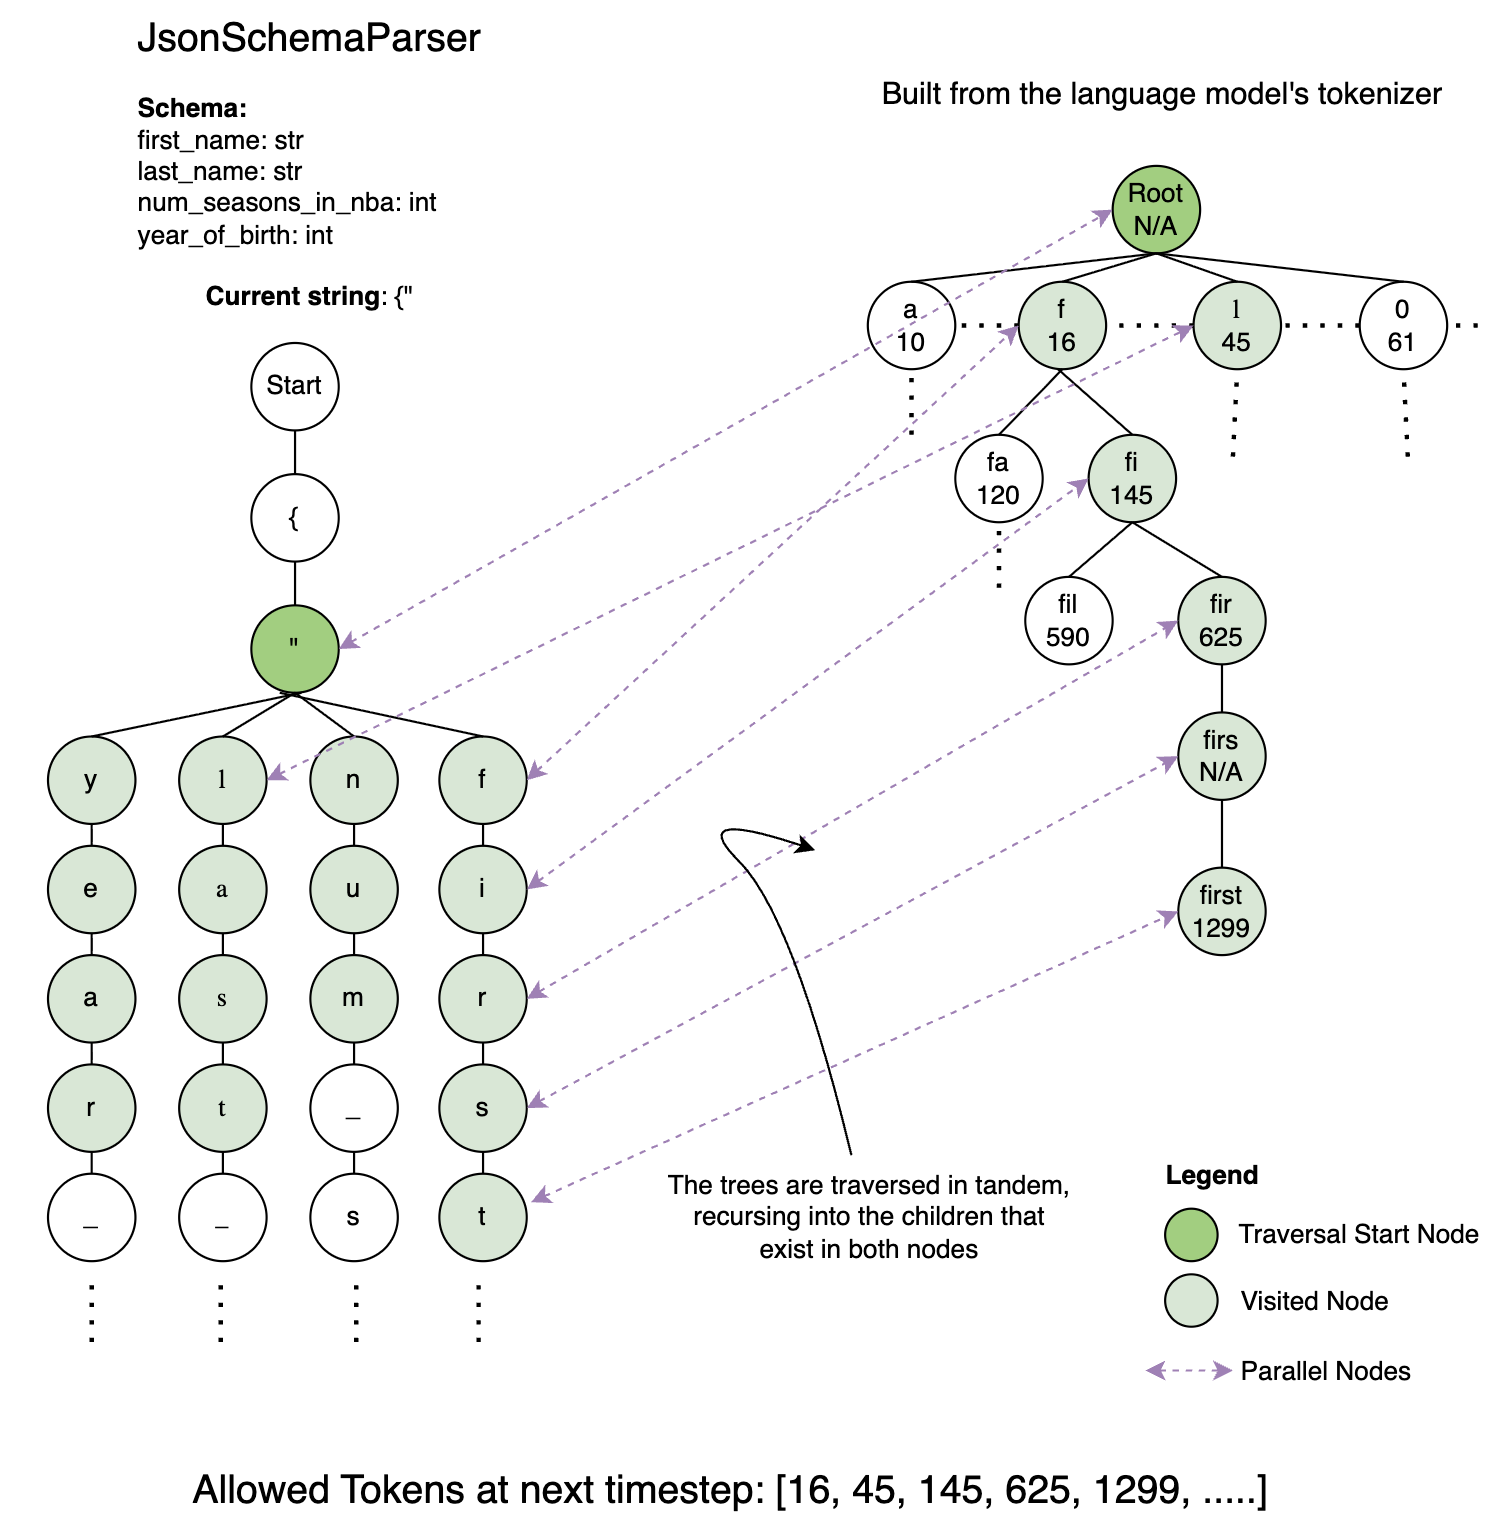
\includegraphics[width=0.7\textwidth]{Bilder/LMFormatEnforcer.png}
    \caption{LM Format Enforcer mechanism: intersecting a character-level parser with a tokenizer prefix tree to constrain structured generation by computing the set of allowed next tokens at each decoding step \cite{noamgat-no-date}.}
    \label{fig:lmfe_mechanism}
\end{figure}
\FloatBarrier

\section{Expert Agents}
\label{sec:Expert_agents}

This section describes the expert agents used in the basic multi-agent experiments. In this first stage of the pipeline, multiple experts assess the same claim in parallel and return structured outputs that can be aggregated into a single binary decision (aggregation strategies are described in the next section). The expert design is intentionally lightweight: experts are defined purely through prompting (role + constraints) and a shared output schema, enabling controlled comparisons across prompt variants and inference settings.

\subsection{Prompt-Based Experts}

The baseline prototype uses three prompt-defined expert agents: \textit{politics}, \textit{economy}, and \textit{health/science}. These three domains were selected because they represent the largest and most distinct topical clusters in the LIAR dataset 
(Section~\ref{sec:exploratory_domain_analysis}), covering the majority of training instances while remaining semantically separable enough to support meaningful domain specialization. All three experts use the same underlying backbone model, but differ in their system prompts, which specify (i) the domain perspective, (ii) the kinds of publicly verifiable evidence to prioritize, and (iii) a conservative decision policy that defaults to \texttt{False} when evidence is insufficient or ambiguous. Concretely:

\begin{itemize}
    \item \textbf{Politics expert.} Focuses on U.S.\ politics, elections, legislation, and public records, emphasizing verifiable sources such as roll calls, bill texts, statutes, and official filings.
    \item \textbf{Economy expert.} Focuses on macroeconomics, labor statistics, budgets, and taxation, emphasizing statistical agencies and budget institutions (e.g., BLS, BEA, CBO, Treasury/IRS) and requiring precise definitions of metrics and time ranges.
    \item \textbf{Health/science expert.} Focuses on healthcare policy, public health, and scientific evidence appraisal, emphasizing institutional sources (e.g., CDC, FDA, NIH, WHO) and peer-reviewed literature, and explicitly distinguishing correlation from causation when relevant.
\end{itemize}

Each expert receives the same claim (statement text) and produces a compact machine-readable JSON object with two fields: a binary verdict (\texttt{True} or \texttt{False}) and a short explanation (2--4 concise sentences). This shared interface is crucial for aggregation because it keeps the expert stage comparable across configurations while allowing domain-specific reasoning through the role prompts.

\paragraph{Subject conditioning}
To test whether topic metadata improves expert judgments, the expert prompts were evaluated both \emph{with} and \emph{without} injecting the LIAR subject string into the input.

\subsection{Fine-Tuned Experts}

For clarity, the experiments compare three expert implementations:
\begin{itemize}
    \item \textbf{Prompt-only backbones:} untuned models instructed via prompts.
    \item \textbf{Domain-general fine-tuning:} LoRA adapters trained on the full LIAR training set.
    \item \textbf{Domain-specific fine-tuning:} LoRA adapters trained on topical LIAR subsets (economy, politics, health/science).
\end{itemize}

Beyond prompt-only experts, two additional expert types use supervised adaptation via LoRA fine-tuning. In both cases, experts retain the same binary label space (\texttt{True}/\texttt{False}) but are trained to align more directly with the LIAR labeling function. For domain-specific fine-tuning, the training data is grouped into three coarse superlabels aligned with the expert roles: \textit{economy}, \textit{politics}, and \textit{health/science}. Separate adapters are trained per superlabel and evaluated on the full LIAR test set.

This design yields \emph{domain-specialized fine-tuned experts}: each expert is optimized on a subset of the training distribution that corresponds to its topical scope, while evaluation on the full LIAR test set provides a measure of cross-domain transfer and robustness. Fine-tuned experts are used in the multi-agent setting analogously to prompt-based experts: each produces an independent binary decision that can be combined by the aggregation mechanisms described in the next section.

\subsection{Domain-General vs.\ Domain-Specific Experts}

The prototype experiments contrast two forms of expertise:

\begin{itemize}
    \item \textbf{Domain-specific experts:} experts whose prompts (or fine-tuning data) target a particular topical area (politics, economy, health/science). The intended advantage is improved precision in the relevant domain, by encouraging the expert to rely on appropriate evidence standards and domain-relevant sources.
    \item \textbf{Domain-general experts:} experts that apply a generic fact-checking instruction without a strong topical constraint, relying on general world knowledge and broad instruction-following behavior. This form is less specialized but can be more robust when claims do not clearly belong to a single domain.
\end{itemize}

In the first multi-agent experiments, domain specificity is realized through prompt-defined roles applied to the untuned backbones. The fine-tuning experiments then introduce two supervised variants: domain-general fine-tuning on the full LIAR training set, and domain-specific fine-tuning on topical subsets aligned with the expert roles. The remainder of this chapter focuses on how expert outputs are aggregated into a single pipeline verdict; routing and additional control modules are introduced in the final framework chapter.

\section{Decision Mechanisms}

This section describes how the prototype multi-agent pipeline aggregates expert outputs into a single binary prediction.
Each expert returns a structured verdict (\texttt{True}/\texttt{False}) with a short justification.
Aggregation maps the set of expert outputs to one final label $\hat{y}$.
All aggregation strategies are evaluated under controlled conditions, keeping expert prompts and structured-output constraints fixed.

\subsection{Final Classification Strategy}
Let $K$ denote the number of experts. Each expert $i \in \{1,\dots,K\}$ produces a binary vote
$y_i \in \{\texttt{True},\texttt{False}\}$.
The pipeline computes the final prediction $\hat{y}$ using one of three aggregation mechanisms:
\begin{itemize}
    \item \textbf{Majority vote:} an unweighted rule where each expert contributes equally.
    \item \textbf{Router-weighted vote:} a weighted rule where a prompted router assigns claim-specific weights $w_i$.
    \item \textbf{Decision-agent aggregation:} a separate model that reads the expert outputs and generates the final verdict.
\end{itemize}

\subsection{Majority Vote}
With $K=3$ experts, majority vote selects the label supported by at least two experts:
\[
\hat{y} = \arg\max_{c \in \{\texttt{True},\texttt{False}\}} \sum_{i=1}^{3} \mathbb{1}[y_i = c].
\]
Because $K$ is odd, ties cannot occur in this setting.

\subsection{Router-Weighted Voting}
To test whether claim--domain alignment improves aggregation, a router assigns non-negative weights $w_i$ to experts on a per-claim basis. The final label is chosen by weighted voting:
\[
\hat{y} = \arg\max_{c \in \{\texttt{True},\texttt{False}\}} \sum_{i=1}^{K} w_i \cdot \mathbb{1}[y_i = c].
\]
Weights are normalized to sum to one, $\sum_{i=1}^{K} w_i = 1$, so that the scale of the vote is comparable across instances. In practice, higher weights are assigned to the expert whose domain is judged most relevant to the claim, while lower weights are assigned to less relevant experts.

\paragraph{Weight estimation.}
Router weights are produced by a separate routing model that predicts claim--domain relevance for the three expert domains (\texttt{politics}, \texttt{economy}, \texttt{health\_science}).
For each backbone family, the router uses the same underlying model as the experts in that configuration (i.e. \textsc{Gemma} routes \textsc{Gemma} experts, \textsc{Llama} routes \textsc{Llama} experts, and \textsc{DeepSeek} routes \textsc{DeepSeek} experts), so routing quality reflects the same base model capabilities as the downstream expert judgments.
The router receives the claim text and optionally the LIAR subject tags and is prompted to output a JSON object with three non-negative values in $[0,1]$.
To enforce a valid output format, generation is constrained using a JSON-schema-based decoder, ensuring that only the required keys are emitted.
The raw router outputs are post-processed by clipping each value to $[0,1]$ and renormalizing to sum to one.
If the router output cannot be parsed, a uniform fallback distribution $w_i=\tfrac{1}{3}$ is used.
The final weights are therefore comparable across instances and can be interpreted as a soft relevance distribution over experts.

\subsection{Decision-Agent Aggregation}
Decision-agent aggregation replaces rule-based voting with an additional adjudication step. A separate decision model receives the structured expert outputs (verdicts and short explanations) and produces the final verdict $\hat{y}$ (and an accompanying explanation). This mechanism can, in principle, discount weak or internally inconsistent expert justifications even when the raw votes are similar.

\paragraph{Structured outputs.} 
For all aggregation mechanisms, both expert responses and the final output are constrained to valid JSON via decoding-time enforcement (LM Format Enforcer), ensuring that intermediate outputs are reliably machine-readable and can be evaluated consistently.

\section{Multi-Agent Evaluation}

This section evaluates the two-stage multi-agent pipeline on the binary LIAR test set.
All systems use the same expert interface (binary verdict + short explanation) and differ only in (i) the expert implementation (prompt-only vs.\ fine-tuned), (ii) the aggregation mechanism, and (iii) whether LIAR subject tags are injected as additional metadata.

\subsection{Evaluation Metrics}

Performance is reported using standard binary classification metrics: accuracy, precision, recall, and $F_1$.
In addition, confusion matrices are provided to expose the underlying error structure (false positives vs.\ false negatives).
Following the binary reduction used throughout this thesis, $\texttt{True}$ is treated as the positive class when reporting precision, recall, and $F_1$.
For aggregation mechanisms (majority vote, weighted vote, decision-agent), metrics are computed on the full test set.

\subsection{Results}

Table~\ref{tab:multiagent_agg_subset} summarizes aggregation-only results for three model families (\textsc{Gemma}, \textsc{Llama}, \textsc{DeepSeek}) across three training regimes (basic model, LIAR-finetuned, domain-specific) and two input conditions (with vs.\ without LIAR subjects). Complete results for all models and configurations are reported in Appendix~E Table~\ref{tab:multiagent_all_results}.

\paragraph{Overall best configurations.}
The strongest results are backbone-dependent.
For \textsc{Gemma}, the best overall Macro-F1 is obtained with the decision-agent in the LIAR-finetuned regime without subjects (Acc $=0.631$, Macro-F1 $=0.604$), while majority voting achieves the highest accuracy in this regime (Acc $=0.644$, Macro-F1 $=0.595$); the gap reflects a more skewed prediction distribution under majority voting.
For \textsc{Llama}, router-weighted voting is consistently the strongest aggregation method, peaking in the LIAR-finetuned regime with subjects (Acc $=0.630$, Macro-F1 $=0.629$).
For \textsc{DeepSeek}, the largest improvement is achieved via domain-specific training combined with majority voting without subjects (Acc $=0.609$, Macro-F1 $=0.608$).

\paragraph{Aggregation mechanisms: decision-agent vs.\ voting.}
Across most settings, the decision-agent does not outperform the strongest voting rule in accuracy, though it sometimes yields a higher Macro-F1 by producing more balanced class predictions.
For \textsc{Gemma} in the LIAR-finetuned regime without subjects, majority voting achieves Acc $=0.644$ and Macro-F1 $=0.595$, while the decision-agent reaches Acc $=0.631$ and Macro-F1 $=0.604$; the higher Macro-F1 of the decision-agent reflects a less skewed prediction distribution despite lower accuracy.
A clearer advantage for voting holds for \textsc{Llama} in the LIAR-finetuned regime with subjects, where decision-agent aggregation (Acc $=0.603$, Macro-F1 $=0.599$) is below weighted voting on both metrics (Acc $=0.630$, Macro-F1 $=0.629$).
These comparisons suggest that rule-based aggregation is the more reliable default in this setting, while the decision-agent does not consistently exploit explanations to correct errors.

\paragraph{Majority vs.\ weighted voting depends on the backbone.}
Weighted voting behaves differently across model families.
For \textsc{Llama}, weighted voting consistently improves over majority voting in every listed training regime and subject condition, on both accuracy and Macro-F1.
For example, in the LIAR-finetuned regime without subjects, weighted voting increases performance from Acc $=0.597$, Macro-F1 $=0.585$ (majority) to Acc $=0.616$, Macro-F1 $=0.614$ (weighted).
With subjects, the gain remains visible (majority: Acc $=0.615$, Macro-F1 $=0.610$; weighted: Acc $=0.630$, Macro-F1 $=0.629$), indicating that routing weights correlate with useful expert selection for this backbone.
In contrast, \textsc{DeepSeek} often favors majority voting over weighted voting, particularly under domain-specific training (no subjects: majority Acc $=0.609$, Macro-F1 $=0.608$ vs.\ weighted Acc $=0.524$, Macro-F1 $=0.506$), suggesting that weighting can amplify failure modes when routing is miscalibrated.

\paragraph{Effect of training regime (basic vs.\ LIAR-finetuned vs.\ domain-specific).}
Training regime effects are strongest for \textsc{DeepSeek}.
In the LIAR-finetuned regime without subjects, majority voting reaches Acc $=0.531$ and Macro-F1 $=0.513$, while domain-specific training increases this to Acc $=0.609$ and Macro-F1 $=0.608$ indicating that role-aligned adaptation substantially stabilizes the expert ensemble for this backbone.
For \textsc{Gemma}, the LIAR-finetuned regime is clearly stronger than the basic model regime; for instance, under majority voting without subjects, performance rises from Acc $=0.549$, Macro-F1 $=0.535$ (basic model) to Acc $=0.644$, Macro-F1 $=0.595$ (LIAR-finetuned).
For \textsc{Llama}, the LIAR-finetuned regime also improves substantially over the basic model regime, but the overall outcome remains strongly controlled by the aggregation choice, with weighted voting consistently yielding the best results.

\begin{table}[t]
\centering
\scriptsize
\setlength{\tabcolsep}{3.5pt}
\renewcommand{\arraystretch}{1.05}
\caption{Aggregation-only results on \texttt{liar\_test} ($n = 1267$). Reported are Accuracy and Macro-F1 (unweighted average of $F_1$ over both classes) for three aggregation mechanisms: decision agent, majority vote, and weighted vote. Best Macro-F1 per row is highlighted in bold.}
\label{tab:multiagent_agg_subset}
\begin{adjustbox}{max width=\textwidth}
\begin{tabular}{@{}l p{2.8cm} c rr rr rr@{}}
\toprule
& & & \multicolumn{2}{c}{Decision Agent} & \multicolumn{2}{c}{Majority Vote} & \multicolumn{2}{c}{Weighted Vote} \\
\cmidrule(lr){4-5} \cmidrule(lr){6-7} \cmidrule(lr){8-9}
Train-Set & Model & Subj. & Acc & MF1 & Acc & MF1 & Acc & MF1 \\
\midrule
basic model     & gemma-7b-it           & no  & 0.551 & 0.539          & 0.549 & 0.535          & \textbf{0.563} & \textbf{0.554} \\
basic model     & gemma-7b-it           & yes & 0.566 & 0.562          & 0.571 & 0.566          & \textbf{0.576} & \textbf{0.572} \\
LIAR-finetuned  & gemma-7b-it           & no  & 0.631 & \textbf{0.604} & \textbf{0.644} & 0.595          & 0.643 & 0.597 \\
LIAR-finetuned  & gemma-7b-it           & yes & 0.627 & 0.610          & \textbf{0.636} & \textbf{0.612} & 0.630 & 0.607 \\
domain-specific & gemma-7b-it           & no  & 0.613 & 0.607          & 0.618 & 0.616          & \textbf{0.631} & 0.605 \\
domain-specific & gemma-7b-it           & yes & 0.631 & 0.624          & \textbf{0.638} & \textbf{0.628} & 0.633 & 0.625 \\
\midrule
basic model     & Llama-3.1-8B-Instruct & no  & 0.474 & 0.413          & 0.470 & 0.392          & \textbf{0.477} & \textbf{0.424} \\
basic model     & Llama-3.1-8B-Instruct & yes & \textbf{0.479} & \textbf{0.427} & 0.473 & 0.399        & 0.474 & 0.421 \\
LIAR-finetuned  & Llama-3.1-8B-Instruct & no  & 0.583 & 0.573          & 0.597 & 0.585          & \textbf{0.616} & \textbf{0.614} \\
LIAR-finetuned  & Llama-3.1-8B-Instruct & yes & 0.603 & 0.599          & 0.615 & 0.610          & \textbf{0.630} & \textbf{0.629} \\
domain-specific & Llama-3.1-8B-Instruct & no  & 0.543 & 0.515          & 0.524 & 0.482          & \textbf{0.565} & \textbf{0.550} \\
domain-specific & Llama-3.1-8B-Instruct & yes & 0.543 & 0.523          & 0.533 & 0.498          & \textbf{0.567} & \textbf{0.555} \\
\midrule
basic model     & deepseek-llm-7b-base  & no  & 0.491 & 0.451          & \textbf{0.496} & \textbf{0.460} & 0.492 & 0.453 \\
basic model     & deepseek-llm-7b-base  & yes & \textbf{0.516} & \textbf{0.500} & 0.507 & 0.488        & 0.514 & 0.493 \\
LIAR-finetuned  & deepseek-llm-7b-base  & no  & 0.502 & 0.470          & \textbf{0.531} & \textbf{0.513} & 0.484 & 0.437 \\
LIAR-finetuned  & deepseek-llm-7b-base  & yes & \textbf{0.525} & \textbf{0.514} & 0.522 & 0.510        & 0.489 & 0.450 \\
domain-specific & deepseek-llm-7b-base  & no  & 0.527 & 0.516          & \textbf{0.609} & \textbf{0.608} & 0.524 & 0.506 \\
domain-specific & deepseek-llm-7b-base  & yes & \textbf{0.519} & \textbf{0.509} & 0.526 & 0.512        & 0.491 & 0.450 \\
\bottomrule
\end{tabular}
\end{adjustbox}
\end{table}

\subsection{Ablation Studies}

Ablations isolate three factors: (i) subject conditioning, (ii) aggregation strategy, and (iii) training regime.

\paragraph{Subject conditioning (with vs.\ without subjects).}
Subject tags show small and inconsistent effects.
For \textsc{Gemma} in the LIAR-finetuned regime, subject injection slightly reduces Macro-F1 under majority voting (from $0.595$ to $0.612$) and weighted voting (from $0.597$ to $0.607$), while the decision-agent improves marginally (from $0.604$ to $0.610$).
For \textsc{Llama}, subject tags tend to help in the strongest configurations: in the LIAR-finetuned regime under weighted voting, Macro-F1 improves from $0.614$ (no subjects) to $0.629$ (with subjects).
For \textsc{DeepSeek}, the effect varies by training regime; in the domain-specific regime, adding subjects reduces majority vote Macro-F1 from $0.608$ (no subjects) to $0.512$ (with subjects), a substantial drop indicating that subject metadata interacts poorly with domain-specific adaptation for this backbone.
Overall, subject metadata behaves as an auxiliary cue that can help under some routing conditions but is not robustly beneficial.

\paragraph{Aggregation ablation: majority vs.\ weighted vs.\ decision-agent.}
Majority vote provides a stable baseline, while weighted voting is beneficial mainly when routing is reliable.
For \textsc{Llama}, weighted voting consistently improves Macro-F1 over majority voting across all regimes and subject settings.
For \textsc{DeepSeek}, majority voting is often preferable in terms of both accuracy and Macro-F1, particularly under domain-specific training where weighted voting underperforms sharply.
Across backbones, decision-agent aggregation is rarely the strongest option: it achieves the best Macro-F1 only for \textsc{Gemma} in the LIAR-finetuned no-subjects regime ($0.604$ vs.\ $0.595$ for majority voting), where its more balanced class predictions yield a small advantage despite lower accuracy.

\paragraph{Training regime ablation: basic vs.\ LIAR-finetuned vs.\ domain-specific.}
Domain-specific training yields the strongest gains for \textsc{DeepSeek}, especially when paired with majority voting without subjects ($\Delta$Macro-F1 $= +0.095$ over LIAR-finetuned majority vote).
For \textsc{Gemma} and \textsc{Llama}, the LIAR-finetuned regime is substantially stronger than the basic model regime, while domain-specific variants remain competitive but do not uniformly surpass the best LIAR-finetuned configurations on Macro-F1.

\paragraph{Summary.}
Taken together, the results indicate that (i) simple voting rules are strong and reliable aggregators, (ii) the usefulness of router-weighted voting is backbone-dependent---consistently beneficial for \textsc{Llama} but counterproductive for \textsc{DeepSeek} under miscalibrated routing---and (iii) domain-specific training is particularly important for stabilizing weaker backbones, as evidenced by the large Macro-F1 gains for \textsc{DeepSeek}. The Macro-F1 metric proves especially informative here: several configurations that appear similar in accuracy differ meaningfully in class balance, with majority voting tending to produce more skewed predictions than the decision-agent in high-recall regimes.

\paragraph{Limitations and motivation for the final framework.}
Despite these improvements over single-model baselines, the prototype reveals three key limitations that motivate the extended framework in Chapter~\ref{chap:final_framework}. First, all claims are evaluated by all three experts regardless of their actual domain, which is inefficient and introduces noise from irrelevant expert perspectives. Second, the three-domain taxonomy is coarse and may not capture the full topical diversity of LIAR. Third, the pipeline has no mechanism to filter non-verifiable or underspecified claims, which forces experts into speculative decisions. These limitations are addressed in the final framework through domain routing, finer-grained taxonomies, and a checkability gate.
  \chapter{Final Domain-Specialized Multi-Agent Framework}
\label{chap:final_framework}

The prototype pipeline presented in Chapter~\ref{chap:prototype_framework} revealed three key limitations. First, all claims were evaluated by all three experts regardless of their actual domain, introducing noise from irrelevant expert perspectives and wasting compute. Second, the coarse three-domain taxonomy (politics, economy, health/science) did not capture the full topical diversity of LIAR, limiting the specialization capacity of individual experts. Third, the pipeline had no mechanism to filter non-verifiable or underspecified claims, forcing experts into speculative decisions on inputs that are inherently difficult to classify.

This chapter addresses each of these limitations through three targeted extensions: (i) a \emph{domain routing model} that assigns 
each claim to the most relevant expert rather than evaluating all claims with all experts, (ii) a \emph{finer-grained taxonomy} with 
up to 13 super-domains to enable more precise specialization, and (iii) a \emph{checkability gate} that filters non-verifiable inputs before they reach the expert pipeline. Together, these components form the final domain-specialized multi-agent framework evaluated in this chapter.

\section{Domain Routing Model}

\subsection{Purpose and Design}

The multi-agent framework relies on a \emph{router} that assigns each input claim to a single high-level domain. This routing step serves two goals: (i) selecting the most relevant \emph{domain-specialized expert}, and (ii) enabling routing-aware aggregation schemes (e.g., router-weighted voting) where expert contributions can be modulated by domain relevance.

Formally, the routing model implements a function
\[
r(\text{claim}) \rightarrow \texttt{super\_domain} \in \mathcal{D},
\]
where $\mathcal{D}$ is a fixed set of super-labels (e.g., 8-way routing). The router operates only on the statement text at inference time. Subjects or metadata are not required for prediction; they are used only to construct weak supervision labels during training.

\paragraph{Backbone-aligned (self) routing.}
To avoid cross-model mismatch, routing is performed using a router built on the same backbone family as the downstream experts (e.g., a Gemma-based router for Gemma experts, a Llama-based router for Llama experts, and a DeepSeek-based router for DeepSeek experts). This keeps domain assignment aligned with the model family's internal representations and reduces inconsistencies that can arise when routing and expert judgment are produced by different model families.

\subsection{Super-Label Taxonomy and Rationale}

To control the granularity of specialization, three alternative super-label taxonomies were explored: a coarse (6 labels), an intermediate (8 labels), and a fine (13 labels) configuration.

\paragraph{8 super-labels.}
\[
\mathcal{D}_{8}=\left\{
\begin{array}{@{}l@{}}
\texttt{economy},\,\texttt{health\_social},\,\texttt{foreign\_security},\,\texttt{law\_rights},\\
\texttt{politics\_government},\,\texttt{environment\_energy},\,\texttt{society\_culture},\,\texttt{misc}\
\end{array}
\right\}.
\]

\paragraph{6 super-labels (coarser grouping).}
\[
\mathcal{D}_{6=}\left\{
\begin{array}{@{}l@{}}
\texttt{socioeconomic\_policy},\,\texttt{foreign\_security},\,\texttt{governance\_law},\\
\texttt{environment\_science},\,\texttt{society\_culture},\,\texttt{misc}
\end{array}
\right\}.
\]

\paragraph{13 super-labels (finer specialization).}
\[
\mathcal{D}_{13}=\left\{
\begin{array}{@{}l@{}}
\texttt{macro\_econ},\ \texttt{jobs\_labor},\ \texttt{business\_finance},\ \texttt{cost\_of\_living\_housing},\\
\texttt{healthcare\_policy},\ \texttt{public\_health\_crises},\ \texttt{substances\_gambling},\\
\texttt{family\_demographics},\,\texttt{law\_crime\_rights},\
\texttt{institutions\_elections},\\ \texttt{foreign\_affairs\_security},\
\texttt{environment\_energy\_infra},\ \texttt{media\_meta}
\end{array}
\right\}.
\]

\subsection{Label Construction from LIAR Subjects}

The LIAR dataset provides a comma-separated \texttt{subjects} field that describes topical tags for each statement. Since the router must predict exactly one domain label, training labels are derived from these tags using a deterministic mapping:
\[
\texttt{subjects} \rightarrow \texttt{super\_domain}.
\]
Concretely, each subject tag is mapped to one super-label via a dictionary (\texttt{domain\_to\_super}). If multiple tags map to multiple super-labels, a single label is chosen using a priority rule determined by the ordered list of \texttt{super\_labels}. If no tag yields a known mapping, the example defaults to \texttt{misc}. This yields a single ``weak supervision'' label per statement.

This approach has two practical advantages: it produces routing labels at scale without manual annotation, and it keeps routing consistent with the dataset's topical organization. Its main limitation is that LIAR subjects can be noisy or incomplete; therefore routing performance reflects both model quality and label quality.

\subsection{Router Model Architecture}

The router is trained as a LoRA adapter on top of an instruction-tuned language model backbone (e.g., \texttt{meta-llama/Llama-3.1-8B-Instruct}).

In the implementation, LoRA is applied to attention and MLP projection modules
\[
\{\texttt{q\_proj},\texttt{k\_proj},\texttt{v\_proj},\texttt{o\_proj},\texttt{gate\_proj},\texttt{up\_proj},\texttt{down\_proj}\},
\]
with rank $r=8$, scaling $\alpha=16$, and dropout $0.05$.

\subsection{Training Objective and Data Formatting}

Routing is trained as a constrained generation problem: given a statement, the model must output exactly one domain label (no explanation). Each training example is formatted as a chat-style sequence:
\begin{itemize}
    \item \textbf{System message:} strict instruction listing valid labels (constructed from the chosen taxonomy),
    \item \textbf{User message:} the claim statement text,
    \item \textbf{Assistant target:} the gold \texttt{super\_domain} label string.
\end{itemize}
Training uses a standard causal language modeling objective on the full chat-formatted input (system + user + label). A language-modeling collator is applied with masked language modeling disabled, and the adapter is optimized for a small number of epochs (e.g., 3) with a learning rate typical for LoRA adapters (e.g., $5\times10^{-4}$).

\subsection{Inference Procedure and Output Normalization}

At inference time, the router receives only the statement text and produces a short completion (e.g., up to 8 new tokens) using greedy decoding (\texttt{do\_sample=False}). To ensure robustness against minor formatting noise, the output label is extracted using a strict normalization heuristic:
\begin{enumerate}
    \item exact word match against the valid label list,
    \item substring fallback if an exact match fails,
    \item default to \texttt{misc} if no label is detected.
\end{enumerate}
This procedure is intentionally strict, aligning with the router's design goal: always return exactly one valid label.

\subsection{Routing Accuracy}

Routing accuracy is evaluated by comparing predicted super-domains against the subject-derived labels on a held-out test split. The evaluation reports overall accuracy, per-class precision/recall/$F_1$, and a confusion matrix (true labels as rows, predicted labels as columns). Because labels are derived from LIAR subjects, reported routing accuracy should be interpreted as agreement with the subject-tag mapping rather than ground-truth topicality.

\paragraph{Statement-only evaluation.}
Although LIAR subject tags can be injected as auxiliary metadata elsewhere in the pipeline, the router is trained and evaluated primarily in a statement-only mode to reflect realistic deployment, where only the claim text is available.

\subsection{Results}

This section reports the empirical performance of the routing models across backbone families and super-domain granularities. The analysis focuses exclusively on routing agreement with subject-derived super-domain labels. Binary verdict performance is discussed in the subsequent section.

\subsubsection{Routing Agreement Across Taxonomies}

Routing accuracy is evaluated on the held-out LIAR test split by comparing predicted super-domains against the deterministic subject-derived labels.

Across all backbone families, routing accuracy decreases consistently as label granularity increases (Table~\ref{tab:main_results}). This pattern is stable and architecture-independent.

\paragraph{Coarse taxonomy ($k=6$).}
Under the 6-label configuration, routing accuracy is highest for all backbones. DeepSeek achieves the strongest performance at $0.788$, followed closely by Gemma ($0.769$) and Llama ($0.766$). The small spread between models indicates that broad topical grouping can be recovered reliably from statement text alone.

\paragraph{Intermediate taxonomy ($k=8$).}
When increasing granularity to 8 super-domains, routing accuracy decreases moderately. DeepSeek reaches $0.744$, Llama $0.740$, and Gemma $0.720$. The performance gap between backbone families becomes slightly more pronounced, but the overall degradation remains controlled.

\paragraph{Fine-grained taxonomy ($k=13$).}
Under fine-grained specialization, routing becomes substantially more challenging. Llama achieves $0.689$, DeepSeek $0.680$, and Gemma $0.642$. This reflects the difficulty of distinguishing semantically adjacent subdomains using short, statement-only inputs.

\subsubsection{Error Patterns}

Inspection of the routing confusion matrices (Appendix~\ref{app:confusion_matrices}) reveals that most errors occur between semantically related categories rather than across unrelated domains. 

For the 13-label taxonomy, common confusions include:
\begin{itemize}
    \item \texttt{macro\_econ} vs.\ \texttt{jobs\_labor},
    \item \texttt{institutions\_elections} vs.\ \texttt{media\_meta},
    \item \texttt{law\_crime\_rights} vs.\ policy-oriented governance categories.
\end{itemize}

Similarly, in the 8-label configuration, confusion primarily occurs between \texttt{economy} and \texttt{politics\_government}, as well as between \texttt{law\_rights} and governance-related domains. 

These patterns are consistent with two factors:
\begin{enumerate}
    \item Short claims often contain overlapping topical cues.
    \item Subject-derived supervision introduces additional noise when multiple LIAR tags map to different super-domains and a single priority-based label must be chosen.
\end{enumerate}

\subsubsection{Backbone Comparison}

Across granularities, DeepSeek achieves the highest routing agreement, followed closely by Llama, while Gemma consistently performs slightly worse under finer taxonomies. However, differences between DeepSeek and Llama remain relatively small. The stronger degradation observed for Gemma under $k=13$ suggests that finer-grained semantic discrimination is more sensitive to backbone-specific representation capacity or training stability.

\subsubsection{Summary}

Routing performance exhibits a clear granularity–accuracy trade-off. Coarser taxonomies yield the highest agreement but provide less specialization capacity for downstream experts. Finer taxonomies enable more precise specialization but increase routing ambiguity and susceptibility to label noise. The intermediate 8-label configuration represents a balanced compromise, maintaining strong routing agreement while preserving meaningful domain differentiation.

\begin{table}[t]
\centering
\caption{Routing agreement across backbones and taxonomy granularities on the LIAR test set ($n = 1267$). Domain accuracy reports agreement with subject-derived super-domain labels.}
\label{tab:main_results}
\begin{tabular}{llrrrrr}
\hline
Backbone & $k$ & Domain acc. \\
\hline
DeepSeek & 6  & 0.788 \\
DeepSeek & 8  & 0.744 \\
DeepSeek & 13 & 0.680 \\
\hline
Llama    & 6  & 0.766 \\
Llama    & 8  & 0.740 \\
Llama    & 13 & 0.689 \\
\hline
Gemma    & 6  & 0.769 \\
Gemma    & 8  & 0.720 \\
Gemma    & 13 & 0.642 \\
\hline
\end{tabular}
\end{table}

\FloatBarrier

\section{Checkability Model}

\subsection{Motivation and Definition}
A recurring issue in benchmark and real-world fact-checking is that not every input is a well-formed, verifiable claim.
In LIAR-style data, some entries are incomplete fragments, topical cues without an assertion, or references that depend on missing context.
Typical examples include: (i) fragmentary statements without a proposition (e.g., ``On the Bush tax cuts .''), (ii) pronoun-only references without a resolvable entity (e.g., ``Says states mandated tests come from an English company .''), and (iii) underspecified claims where key information such as actor, time, or location is missing.
Such cases introduce noise into both training and evaluation and can force downstream agents into guessing behavior.

To mitigate this, the pipeline introduces a \emph{checkability gate} that determines whether a statement is suitable for automated fact-checking.
Checkability is operationalized as a categorical decision:
\[
\mathrm{checkability}(x) \in \mathcal{C},
\]
where $\mathcal{C}$ is a small set of mutually exclusive categories.
Only statements labeled as \texttt{fact\_checkable} are forwarded to the domain router and expert agents.

\subsection{Checkability Categories}
The checkability model predicts exactly one of the following categories:
\begin{itemize}
    \item \texttt{fact\_checkable}: a concrete factual claim that can be verified with objective evidence (e.g., dates, votes, laws, numerical assertions).
    \item \texttt{non\_claim}: no clear factual proposition (topic headings, fragments, or descriptive placeholders).
    \item \texttt{opinion\_or\_ambiguous}: primarily evaluative language, vague blame, or claims without a clear factual benchmark.
    \item \texttt{needs\_additional\_context}: potentially checkable in principle, but missing essential context (who/what/when/where).
    \item \texttt{sensitive\_selfharm}: statements about suicide/self-harm that are ethically sensitive and excluded from automatic True/False assignment.
\end{itemize}

This design separates \emph{ill-posed} inputs (e.g., \texttt{non\_claim}) from \emph{underspecified} inputs (e.g., \texttt{needs\_additional\_context}) and additionally isolates sensitive content into a dedicated category.

\subsection{Modeling and Output Format}
The checkability component is implemented as a lightweight classifier using an instruction-following language model in \emph{generation mode}.
Given a statement, the model is prompted to return \emph{only} a JSON object of the form:
\[
\{\texttt{"category"}:\ \cdots\}.
\]
No explanation, markdown, or additional keys are permitted.
At inference time, the system extracts the first valid JSON object from the generated text; if parsing fails, it falls back to a conservative default category (implemented as \texttt{opinion\_or\_ambiguous} in the current pipeline).

Importantly, the checkability gate uses the \emph{base model} (without LoRA adapters), since its purpose is not domain specialization but robust detection of malformed or underspecified inputs.

\subsection{Pipeline Integration}
The checkability gate is placed \emph{before} routing and expert evaluation:
\begin{enumerate}
    \item \textbf{Checkability filtering:} assign a checkability category $\in \mathcal{C}$.
    \item \textbf{Domain routing:} for \texttt{fact\_checkable} inputs, predict exactly one super-domain label.
    \item \textbf{Domain expert:} run the domain-specific expert to produce \texttt{True}/\texttt{False} plus a short explanation.
    \item \textbf{Optional escalation:} if enabled, apply an additional adjudication step (e.g., a generalist tie-breaker or second-expert fallback).
\end{enumerate}

Only statements categorized as \texttt{fact\_checkable} are forwarded to subsequent stages.
All other categories are excluded from True/False prediction to avoid forcing domain experts into speculative decisions.

\subsection{Evaluation Handling}
Depending on the reporting setup, non-checkable inputs are handled in one of two ways:
\begin{itemize}
    \item \textbf{Filtered evaluation:} remove non-checkable instances and compute routing and verdict metrics only on the \texttt{fact\_checkable} subset.
    \item \textbf{Separate accounting:} track excluded instances as a dedicated category and report their frequency alongside standard classification metrics.
\end{itemize}

In the implemented evaluation routine, routing accuracy and fact-checking metrics (accuracy, classification report, confusion matrix) are computed on the \texttt{fact\_checkable} subset to ensure comparability across aggregation methods and to prevent ill-posed inputs from dominating error patterns.

\subsection{User-Facing Feedback and Practical Deployment}
In this thesis, the checkability model is primarily used as an \emph{internal filter} to improve the reliability of the downstream evaluation.
The goal is to reduce noise introduced by ill-posed inputs (e.g., fragments or missing referents) and thereby obtain more meaningful accuracy comparisons between routing and aggregation variants.

In a real-world deployment, however, the checkability stage would ideally serve a second purpose: \emph{user-facing guidance}.
In an interactive verification setting (e.g., via an API where users submit claims for checking), the checkability output can be surfaced to the user to explain \emph{why} a claim cannot currently be verified and what information is missing.
For instance, the model can indicate that a statement lacks a named entity, a time reference, or a concrete proposition, and it could prompt the user to provide the required context before a True/False decision is attempted.

This user-feedback functionality is not implemented as part of the experimental pipeline in this work, since the primary objective is improving and analyzing end-to-end classification performance on Fake News.
Nevertheless, for public-facing fact-checking tools, exposing checkability feedback is an important design choice: it improves transparency, reduces misleading binary outputs on underspecified claims, and supports iterative refinement of user queries toward verifiable statements.

\subsection{Results}

Because no ground-truth checkability annotations are available for LIAR, the checkability
component cannot be evaluated in terms of classification accuracy. Instead, the
\emph{empirical category distribution} induced by the gate is reported, i.e.\ how often each base model
assigns statements to \texttt{fact\_checkable} versus exclusion categories. This directly
determines the effective evaluation subset for downstream routing and expert verdicts.

Table~\ref{tab:checkability_dist} summarizes the observed distributions on the test split
($n=1267$). The results show substantial variation across base models. DeepSeek is highly
permissive and classifies almost the entire test set as \texttt{fact\_checkable}
(1263/1267; 99.7\%). Llama filters a moderate fraction of statements (1100/1267; 86.8\%),
primarily assigning the remainder to \texttt{opinion\_or\_ambiguous} and \texttt{non\_claim}.
In contrast, Gemma is considerably stricter, marking fewer than half of all statements as
\texttt{fact\_checkable} (535/1267; 42.2\%), with a large share assigned to
\texttt{needs\_additional\_context} (383/1267; 30.2\%) and \texttt{opinion\_or\_ambiguous}
(279/1267; 22.0\%).

These findings indicate that checkability gating is not a neutral preprocessing step but a
model-dependent decision rule that can substantially alter the downstream evaluation set.
Accordingly, the gate is treated as an explicit, auditable stage of the pipeline: category
frequencies are reported, and routing and verdict metrics are computed only on the
\texttt{fact\_checkable} subset when the gate is enabled.

\begin{table}[t]
\centering
\caption{Checkability gate category distribution on the test split ($n=1267$) using different base models.}
\label{tab:checkability_dist}
\small
\begin{tabular}{lrrrrr}
\toprule
Base model & fact\_checkable & opinion/ambig. & non\_claim & needs\_ctx & selfharm \\
\midrule
Llama    & 1100 (86.8\%) & 122 (9.6\%)  &  42 (3.3\%) &   1 (0.1\%) & 2 (0.2\%) \\
Gemma    &  535 (42.2\%) & 279 (22.0\%) &  68 (5.4\%) & 383 (30.2\%) & 2 (0.2\%) \\
DeepSeek & 1263 (99.7\%) &   2 (0.2\%)  &   2 (0.2\%) &   0 (0.0\%) & 0 (0.0\%) \\
\bottomrule
\end{tabular}
\normalsize
\end{table}

\subsection{Discussion}

The checkability gate increases robustness by explicitly separating \emph{claim understanding}
from \emph{claim verification}. In principle, this reduces noise originating from fragments and
underspecified inputs that would otherwise force downstream experts into speculative
True/False decisions.

At the same time, the empirical results reveal strong \emph{model dependence} in checkability
judgments. A permissive gate (as observed for DeepSeek) largely preserves the original benchmark
distribution but provides limited filtering. A stricter gate (as observed for Gemma) excludes a
substantial fraction of the test set, potentially removing genuinely verifiable but short claims
and thereby altering the effective evaluation subset. Llama exhibits intermediate behavior
between these two extremes.

Consequently, the checkability component is treated as an explicit, auditable stage rather than
an implicit preprocessing heuristic. Category frequencies are reported, and—when the gate is
enabled—routing and verdict metrics are computed exclusively on the
\texttt{fact\_checkable} subset. This approach makes the impact of filtering transparent and
allows downstream comparisons to be interpreted in light of the induced selection effect.

\section{Domain-Specific Agents}

\subsection{Training Procedure}
For each super-domain $d \in \mathcal{D}$, a dedicated expert agent is trained via a lightweight LoRA adapter on top of a shared instruction-tuned backbone (e.g., \texttt{meta-llama/Llama-\\3.1-8B-Instruct}). All experts within the same model family use the \emph{same frozen base model}, but each domain expert has its \emph{own} adapter parameters.

\paragraph{Domain-restricted supervision.}
Expert training data is constructed by filtering the global training set by the domain label:
\[
\mathcal{T}_d = \{(x_i, y_i) \mid \texttt{super\_domain}(x_i)=d\},
\]
where $x_i$ is the claim statement and $y_i \in \{\texttt{True},\texttt{False}\}$ is the binary ground-truth label. Each expert is therefore optimized only on examples from its assigned domain.

\paragraph{Chat-formatted training objective.}
Training is implemented as supervised next-token prediction on a chat-style transcript. Each example is formatted as:
(i) a domain-specific system instruction that defines the expert role, 
(ii) a user message containing the claim text, and
(iii) an assistant target consisting of the gold label (\texttt{True} or \texttt{False}) with no additional text.
The objective encourages the model to generate a single binary verdict under a strict instruction-following interface.

\paragraph{LoRA setup.}
Adapters are trained with rank $r=8$, $\alpha=16$, and dropout $0.05$, applied to the attention and MLP projection modules (\texttt{q\_proj}, \texttt{k\_proj}, \texttt{v\_proj}, \texttt{o\_proj}, \texttt{gate\_proj}, \texttt{up\_proj}, \texttt{down\_proj}). Unless otherwise noted, experts are trained for 3 epochs with learning rate $5\times10^{-4}$, batch size 4, and gradient accumulation of 2. After training, only the LoRA weights and tokenizer are saved in a domain-specific subdirectory.

\paragraph{Memory-efficient sequential execution.}
At inference time, the system is implemented in a memory-efficient sequential manner. After routing has assigned each claim to a domain, experts are loaded one-by-one and applied only to the subset of claims routed to their domain. The corresponding model is then released before the next expert is loaded. This sequential strategy reduces peak VRAM usage and enables evaluation across multiple domain experts without requiring simultaneous multi-model residency.

\subsection{Design Differences}
All domain experts follow a shared interface: they output a binary verdict and a short explanation. Concretely, each expert produces a JSON object with the fields
\[
\texttt{verdict} \in \{\texttt{True}, \texttt{False}\}, \qquad
\texttt{explanation} \ \text{(2--4 concise sentences)}.
\]

\paragraph{Training vs.\ inference interface.}
While inference outputs include both \texttt{verdict} and \texttt{explanation}, the expert adapters are trained using only the binary label supervision (\texttt{True}/\texttt{False}). Explanations are generated at inference time under explicit prompting, as they are not required for the classification objective.

\paragraph{Schema enforcement and fallback behavior.}
To guarantee machine-readable outputs, generation is constrained by a JSON schema (enforced during decoding). If the model produces malformed JSON or cannot be parsed reliably, a deterministic fallback policy is applied (e.g., defaulting to \texttt{False} and attaching a short error note). This ensures that the end-to-end pipeline remains robust and does not break due to occasional formatting errors.

\subsection{Results}

Domain experts are evaluated on the test split using \emph{domain-restricted ground truth}:
for each super-domain $d$, the corresponding expert is applied only to instances whose
gold label satisfies $\texttt{super\_domain}(x)=d$. This isolates expert performance from
routing effects and measures how well each adapter performs on the domain distribution it
was trained for. Performance is reported in terms of accuracy, per-class precision/recall,
and the confusion matrix for the binary labels (\texttt{True}, \texttt{False}).

\paragraph{Overall performance across model families.}
Table~\ref{tab:expert_overall_summary} summarizes overall expert accuracy and macro-F1 when
aggregating all domains for a fixed $(\textit{backbone},k)$ configuration.\footnote{For
$k{=}13$, evaluation covers $n{=}1230$ instances due to domain label availability in the
corresponding split; for $k{=}6$ and $k{=}8$, $n{=}1267$.}
Across all configurations, Llama yields the strongest and most stable expert performance
(mean accuracy $0.663$; mean macro-F1 $0.654$ across $k\in\{6,8,13\}$). Gemma performs
consistently below Llama (mean accuracy $0.627$; mean macro-F1 $0.567$), while DeepSeek
shows the largest variance across $k$ and tends to degrade as the number of domains
increases (mean accuracy $0.635$; mean macro-F1 $0.569$).

\paragraph{Effect of domain granularity.}
Increasing the number of super-domains changes both the training regime (less data per expert)
and the semantic specificity required of each expert.
For Llama, overall accuracy remains relatively stable across $k$ (0.669 at $k{=}6$,
0.660 at $k{=}8$, 0.662 at $k{=}13$), indicating that the adapters retain useful
specialization even under finer domain splits.
Gemma exhibits a mild decline with increasing granularity (0.633 $\rightarrow$ 0.626
$\rightarrow$ 0.621).
DeepSeek shows the strongest decline (0.658 $\rightarrow$ 0.635 $\rightarrow$ 0.613),
suggesting sensitivity to smaller per-domain training sets and/or more brittle instruction
following under finer label spaces.

\paragraph{Class imbalance and prediction bias.}
As noted in Section~\ref{sec:exploratory_domain_analysis}, the LIAR training set 
exhibits a moderate class imbalance (approximately 56\% true vs.\ 44\% false), 
which is reflected in the behavior of several expert configurations. These exhibit 
a tendency toward predicting \texttt{True} more often than \texttt{False}, reflected 
by substantially higher recall for \texttt{True} than for \texttt{False}. This is 
most pronounced for Gemma and DeepSeek. For example, Gemma achieves high recall for 
\texttt{True} (often above 0.88 in the aggregated reports) but comparatively low 
recall for \texttt{False}, producing confusion matrices dominated by \texttt{False} 
$\rightarrow$ \texttt{True} errors. DeepSeek shows a similar pattern for multiple 
domains and, in some small domains, collapses to predicting a single class (e.g., 
near-zero recall for \texttt{False}). In contrast, Llama's class-wise 
precision/recall is more balanced, which is reflected in consistently higher macro-F1.

\paragraph{Per-domain expert performance.}
Per-domain results reveal that performance depends strongly on domain size and label
distribution. Larger domains such as \texttt{socioeconomic\_policy} ($k{=}6$) and
\texttt{economy} ($k{=}8$) yield comparatively stable accuracies across backbones,
whereas small domains (e.g., \texttt{substances\_gambling}, \texttt{public\allowbreak\_health\_crises})
display high variance and are especially prone to single-class behavior, which inflates
accuracy when one label dominates but reduces macro-F1 substantially. This effect is visible
for multiple backbones at $k{=}13$, where some small domains show confusion matrices with
zero predicted instances for one class.

\paragraph{Summary.}
Overall, the expert-only evaluation indicates that (i) domain specialization via LoRA is
effective, but (ii) stability depends on the backbone and the amount of domain-specific
training data. Llama provides the best trade-off between accuracy and balanced class
behavior across all domain granularities, while Gemma and DeepSeek more frequently show
label bias and instability in low-resource domains. A detailed breakdown of all per-domain expert results is provided in Appendix~\ref{tab:expert_per_domain} and Appendix~\ref{tab:expert_summary}.

\begin{table}[t]
\centering
\caption{Expert-only performance aggregated across all domains for each backbone and domain granularity $k$.
Macro-F1 is computed over the two labels \texttt{True}/\texttt{False}.}
\label{tab:expert_overall_summary}
\small
\begin{tabular}{lrrr}
\toprule
Backbone ($k$) & $n$ & Accuracy & Macro-F1 \\
\midrule
Llama ($k{=}6$)  & 1267 & 0.669 & 0.660 \\
Llama ($k{=}8$)  & 1267 & 0.660 & 0.650 \\
Llama ($k{=}13$) & 1230 & 0.662 & 0.652 \\
\midrule
Gemma ($k{=}6$)  & 1267 & 0.633 & 0.569 \\
Gemma ($k{=}8$)  & 1267 & 0.626 & 0.567 \\
Gemma ($k{=}13$) & 1230 & 0.621 & 0.564 \\
\midrule
DeepSeek ($k{=}6$)  & 1267 & 0.658 & 0.622 \\
DeepSeek ($k{=}8$)  & 1267 & 0.635 & 0.561 \\
DeepSeek ($k{=}13$) & 1230 & 0.613 & 0.525 \\
\bottomrule
\end{tabular}
\normalsize
\end{table}

\section{End-to-End Evaluation}

\subsection{Setup and Metrics}
End-to-end performance is evaluated on the binary LIAR test set using the full pipeline
\[
\text{checkability} \rightarrow \text{routing} \rightarrow \text{domain expert}.
\]
The primary outcome is the final binary verdict (\texttt{True}/\texttt{False}), evaluated with
accuracy, precision, recall, and $F_1$ (treating \texttt{True} as the positive class). In addition,
domain routing accuracy is reported to separate errors caused by misrouting from errors caused by
the domain experts themselves. Confusion matrices are included to expose the error structure.

Three taxonomies are compared: $k \in \{6,8,13\}$ domains. For each backbone (Llama, Gemma,
DeepSeek), routing is performed by the corresponding router model, and the final verdict is
generated by the routed domain expert.

\subsection{End-to-End Results without Checkability}
Table~\ref{tab:best_routing_no_gate} summarizes end-to-end verdict performance and routing accuracy
without checkability gating. Across backbones, the 8-domain setting yields the most stable
trade-off between routing difficulty and expert specialization. Llama achieves its strongest
end-to-end accuracy at $k{=}13$ (0.635) and a comparable result at $k{=}8$ (0.632), while $k{=}6$
performs substantially worse (0.543). This degradation is reflected in the confusion matrix, where
$k{=}6$ exhibits a strong bias toward predicting \texttt{False} (high false negatives for
\texttt{True}), suggesting that coarse experts and/or prompting lead to conservative behavior.

DeepSeek attains its best end-to-end accuracy at $k{=}6$ (0.661), while its
performance decreases for finer taxonomies ($k{=}8$: 0.610; $k{=}13$: 0.609),
indicating a monotonic decline as granularity increases. Gemma shows the lowest
overall performance without checkability gating, but its accuracy improves
consistently with larger $k$ ($k{=}6$: 0.489, $k{=}8$: 0.577, $k{=}13$: 0.593),
and the curve shows no sign of flattening at $k{=}13$. LLaMA's pattern is
intermediate: accuracy rises sharply from $k{=}6$ (0.543) to $k{=}8$ (0.632) and
then flattens at $k{=}13$ (0.635), suggesting that the optimum lies near or just
beyond $k{=}13$ for this backbone.

A notable asymmetry therefore emerges across backbones: DeepSeek's accuracy
maximum is at the coarsest taxonomy ($k{=}6$), while LLaMA and Gemma reach
their best results at the finest taxonomy evaluated ($k{=}13$). This divergence
reflects the interaction between routing degradation and expert specialization
gain. For DeepSeek, domain-specific adapters are more sensitive to reduced
per-domain training data, so routing degradation at higher $k$ dominates and
accuracy peaks early. For LLaMA and Gemma, the experts benefit sufficiently
from narrower training distributions to offset the increased routing difficulty,
so the accuracy maximum is pushed toward finer granularities. The practical
implication is that the optimal taxonomy depth is backbone-specific and should
be tuned jointly with expert quality rather than determined from routing accuracy
alone.

\FloatBarrier
\begin{table}[t]
\centering
\caption{Best end-to-end configuration per backbone by verdict accuracy 
\textbf{without} checkability gating on the full test set ($n{=}1267$).}
\label{tab:best_routing_no_gate}
\small
\begin{tabular}{llrrrr}
\toprule
Backbone & $k$ & $n$ & Verdict Acc. & Macro-F1 & Routing Acc. \\
\midrule
DeepSeek & 6  & 1267 & 0.661 & 0.621 & 0.788 \\
Llama    & 13 & 1267 & 0.635 & 0.631 & 0.689 \\
Gemma    & 13 & 1267 & 0.593 & 0.574 & 0.642 \\
\bottomrule
\end{tabular}
\normalsize
\end{table}

\subsection{End-to-End Results with Checkability Gating}
When checkability gating is enabled, evaluation is performed on the subset classified as
\texttt{fact\_checkable} by the gate. This changes the effective test set size in a
model-dependent manner: Llama retains 1100/1267 instances, DeepSeek retains 1263/1267, and Gemma
retains only 535/1267. Table~\ref{tab:best_routing_gate} reports results on these filtered
subsets.

For Llama, checkability gating has little effect on end-to-end verdict accuracy in absolute terms:
$k{=}6$ remains unchanged (0.543 on 1100 instances), $k{=}8$ increases slightly (0.632$\rightarrow$0.637),
and $k{=}13$ decreases marginally (0.635$\rightarrow$0.634). Routing accuracy remains similar across
settings (e.g., $k{=}13$: 0.689$\rightarrow$0.684). This suggests that the main effect of gating for
Llama is selection (changing which claims are evaluated), rather than systematically increasing
or decreasing pipeline competence.

For DeepSeek, gating is nearly neutral because the gate is highly permissive (1263/1267 retained).
Consequently, verdict accuracy and routing accuracy remain essentially unchanged across $k$.

For Gemma, gating substantially alters the evaluated subset due to strict filtering (535/1267
retained). On this reduced subset, verdict accuracy increases compared to the ungated setting for
$k{=}8$ and $k{=}13$ (e.g., $k{=}13$: 0.593$\rightarrow$0.632), while $k{=}6$ remains low (0.489$\rightarrow$0.434).
However, this improvement cannot be interpreted as a pure capability gain because it is confounded
with the strong selection effect induced by the gate. The gated evaluation reflects performance on
claims that Gemma itself considers checkable, rather than on the original benchmark distribution.

\begin{table}[t]
\centering
\caption{Best end-to-end configuration per backbone by verdict accuracy \textbf{with} 
checkability gating. $n$ varies by model due to model-dependent filtering 
(Llama: 1100, Gemma: 535, DeepSeek: 1263).}
\label{tab:best_routing_gate}
\small
\begin{tabular}{llrrrr}
\toprule
Backbone & $k$ & $n$ & Verdict Acc. & Macro-F1 & Routing Acc. \\
\midrule
DeepSeek & 6  & 1263 & 0.661 & 0.624 & 0.787 \\
Llama    & 8  & 1100 & 0.637 & 0.621 & 0.744 \\
Gemma    & 13 &  535 & 0.632 & 0.560 & 0.630 \\
\bottomrule
\end{tabular}
\normalsize
\end{table}

\subsection{Routing vs.\ Expert Errors}
The results indicate that routing constitutes a persistent bottleneck. Even when per-domain experts
are specialized, end-to-end verdict performance is bounded by routing quality, especially at
$k{=}13$, where routing accuracy drops across backbones. Conversely, strong routing does not
guarantee strong end-to-end performance: several settings exhibit reasonable domain accuracy
($\approx$0.74--0.79) while final verdict accuracy remains substantially lower (e.g., Llama/Gemma
at $k{=}6$), implying that expert decision quality and calibration remain limiting factors.

Overall, the 8-domain taxonomy provides the most consistent end-to-end behavior across backbones,
balancing routing reliability with meaningful domain specialization.
  \chapter{Comparative Results and Analysis}
\label{chap:comparative}

This chapter consolidates the empirical findings from the single-model baselines (Chapter~\ref{chap:baseline_single}), the prototype multi-agent pipeline (Chapter~\ref{chap:prototype_framework}), and the final domain-specialized framework (Chapter~\ref{chap:final_framework}) into a unified comparative analysis. The analysis is structured around the three research questions of this thesis: RQ1a (does domain-aware modeling improve binary claim verification accuracy over domain-agnostic aselines?), RQ1b (how well do domain-aware approaches generalize across domains?), and RQ2 (does a multi-agent architecture with domain routing and aggregation outperform single-model fine-tuning?). The goal is to identify overarching performance trends, characterize the conditions under which each design choice provides the greatest benefit, and articulate the fundamental trade-offs between specialization, generalization, and inference cost.

\section{Performance Summary}

Table~\ref{tab:consolidated} summarizes the strongest result obtained at each experimental stage for each backbone family, measured by accuracy and Macro-F1 on the binary LIAR test set ($n = 1267$). Results are drawn from the best single configuration reported in each chapter, selected by accuracy, and are presented without checkability gating to preserve comparability across the full test set. Macro-F1 is the unweighted average of $F_1$ over both classes (True and False); $F_1(+)$ denotes the positive-class $F_1$ for the True class.

\begin{table}[!htbp]
\centering
\scriptsize
\setlength{\tabcolsep}{4pt}
\renewcommand{\arraystretch}{1.2}
\caption{Best-performing configuration per experimental stage and backbone on the LIAR test set ($n = 1267$). Configurations selected by accuracy within each stage. Macro-F1 is the unweighted average of $F_1$ over both classes; $F_1(+)$ denotes $F_1$ for the positive class (True). Dashes indicate that $F_1(+)$ was not computed for prompt-only configurations. All values sourced from Appendix tables.}
\label{tab:consolidated}
\begin{tabular}{l l l r r r}
\toprule
Stage & Backbone & Configuration & Acc & Macro-F1 & $F_1(+)$ \\
\midrule
\multirow{3}{*}{\shortstack[l]{Zero-shot /\\Prompt-only (Ch.~4)}}
  & Gemma-7B-IT           & Reprompting, with subjects              & 0.616 & 0.584 & -- \\
  & LLaMA-3.1-8B-Instruct & P1\_fake\_news\_no\_guess, with subjects & 0.579 & 0.579 & -- \\
  & DeepSeek-LLM-7B       & P2\_one-shot, no subjects               & 0.568 & 0.531 & -- \\
\midrule
\multirow{3}{*}{\shortstack[l]{Single-model\\Fine-Tuning (Ch.~4)}}
  & LLaMA-3.1-8B-Instruct & LIAR-trained, with subjects             & 0.667 & 0.649 & 0.729 \\
  & Gemma-7B-IT           & LIAR-trained, no subjects               & 0.657 & 0.634 & 0.726 \\
  & DeepSeek-LLM-7B       & LIAR-trained, no subjects               & 0.667 & 0.645 & 0.734 \\
\midrule
\multirow{3}{*}{\shortstack[l]{Prototype\\Multi-Agent (Ch.~5)}}
  & Gemma-7B-IT           & LIAR-finetuned, majority vote, no subj. & 0.644 & 0.595 & 0.735 \\
  & LLaMA-3.1-8B-Instruct & LIAR-finetuned, weighted vote, w/ subj. & 0.630 & 0.629 & 0.615 \\
  & DeepSeek-LLM-7B       & Domain-specific, majority vote, no subj.& 0.609 & 0.608 & 0.629 \\
\midrule
\multirow{3}{*}{\shortstack[l]{Final Framework\\(Ch.~6)}}
  & DeepSeek-LLM-7B       & $k{=}6$, no gate                        & 0.661 & 0.621 & 0.742 \\
  & LLaMA-3.1-8B-Instruct & $k{=}13$, no gate                       & 0.635 & 0.631 & 0.677 \\
  & Gemma-7B-IT           & $k{=}13$, no gate                       & 0.593 & 0.574 & 0.667 \\
\bottomrule
\end{tabular}
\end{table}

Three patterns are immediately visible. First, supervised fine-tuning substantially improves over zero-shot prompting for all backbone families: the largest gains are observed for LLaMA and DeepSeek, where accuracy increases from 0.579 and 0.568 to 0.667 respectively. Second, the prototype multi-agent pipeline does not improve over single-model fine-tuning on aggregate metrics for any backbone, with performance gaps ranging from $-0.013$ accuracy (Gemma) to $-0.058$ accuracy (DeepSeek). Third, the final domain-specialized framework narrows but does not close the gap to single-model fine-tuning for LLaMA ($k{=}13$: Acc~=~0.635) and DeepSeek ($k{=}6$: Acc~=~0.661), while Gemma remains the furthest below its fine-tuned baseline ($k{=}13$: Acc~=~0.593).

A cross-stage pattern also emerges in the relationship between accuracy and Macro-F1. For the multi-agent stage, Gemma achieves the highest accuracy (0.644) but the lowest Macro-F1 (0.595) among the three backbones, reflecting a skewed prediction distribution under majority voting. In contrast, LLaMA's multi-agent configuration achieves the highest Macro-F1 (0.629) with only modestly lower accuracy (0.630), indicating more balanced class predictions. This divergence between accuracy and Macro-F1 recurs throughout the experiments and motivates reporting both metrics throughout this chapter.

\section{Research Questions Revisited}

This section addresses the three research questions of this thesis directly, drawing on the empirical results across all experimental stages. For each question, the evidence is organized along the progression from single-model baselines (Chapter~\ref{chap:baseline_single}) through the prototype multi-agent pipeline (Chapter~\ref{chap:prototype_framework}) to the final domain-specialized framework (Chapter~\ref{chap:final_framework}).

\subsection{RQ1a: Does Domain-Aware Modeling Improve Accuracy?}

Domain-aware modeling consistently improves binary claim verification accuracy over domain-agnostic baselines across all experimental stages, but the magnitude of the improvement depends on how domain knowledge is incorporated.

\paragraph{Prompt level.}
Subject conditioning improved LLaMA's Macro-F1 from 0.514 to 0.568 under Setup~B, and the P4 prompt (subjects as context clues) produced the strongest prompt-only result overall (Gemma: Acc~=~0.615, Macro-F1~=~0.586). These gains were model-dependent and did not generalize consistently across architectures: Gemma showed small decreases under some subject-conditioned configurations, and DeepSeek did not benefit consistently from subject injection.

\paragraph{Fine-tuning level.}
Domain-specific LoRA adapters improved in-domain performance for all backbone families. Healthcare-trained LLaMA reached 0.711 accuracy on the healthcare test subset, compared to 0.667 on the general LIAR benchmark. Taxes-trained Gemma reached 0.650 on the taxes subset. These results show that domain-restricted training produces measurable improvements when evaluated within the target domain.

\paragraph{Multi-agent level.}
Domain-specialized expert agents with routing achieved the closest approximation to single-model fine-tuning performance for DeepSeek ($k{=}6$: Acc~=~0.661, Macro-F1~=~0.621) and LLaMA ($k{=}13$: Acc~=~0.635, Macro-F1~=~0.631), demonstrating that structured domain decomposition recovered much of the performance lost in the transition from single-model to multi-agent architectures.

Across all three levels of domain integration, accuracy improvements over domain-agnostic baselines are observed when domain information is structurally incorporated through routing or domain-restricted fine-tuning. Prepending subject metadata alone produces smaller and less consistent gains.

\subsection{RQ1b: How Well Do Domain-Aware Approaches Generalize?}

Domain-aware approaches consistently exhibit a specialization--generalization trade-off: in-domain performance improves, but cross-domain generalization degrades. This pattern is robust across all backbone families and levels of domain granularity.

\paragraph{Single-model fine-tuning.}
Healthcare-trained adapters dropped from 0.711 (in-domain) to 0.650 on the general LIAR test set. Taxes-trained adapters showed a steeper drop, from 0.650 (in-domain) to 0.609 on LIAR. Synthetic-trained adapters demonstrated the most severe distribution mismatch: accuracy of 0.885 on synthetic test data collapsed to 0.604 on LIAR. Subject metadata produced inconsistent generalization effects: in some configurations it improved precision at the cost of recall shifts, suggesting that models exploited topic--label correlations rather than performing genuine claim-level reasoning.

\paragraph{Multi-agent framework.}
Cross-domain generalization in the multi-agent setting is mediated by routing quality. When routing assigns a claim to the correct expert, in-domain performance is maintained. When routing fails -- as is more frequent at finer granularities -- the routed expert operates outside its training distribution, compounding the generalization loss. At $k{=}13$, routing accuracy dropped to 0.64--0.69, directly limiting end-to-end performance for all backbones.

\paragraph{LIAR-specific context.}
The LIAR dataset consists predominantly of short political claims that frequently span multiple topical domains simultaneously. A claim about healthcare spending, for example, simultaneously touches on economic, political, and health domains. This multi-domain character of short political claims means that clean domain boundaries are difficult to maintain, which contributes to the observed generalization losses across all backbone families and domain granularities. Furthermore, because the system operates without external evidence retrieval, domain-specific knowledge cannot be supplemented at inference time, making adapters entirely dependent on patterns learned from the training distribution.

\subsection{RQ2: Does the Multi-Agent Architecture Outperform Single-Model Fine-Tuning?}

On aggregate accuracy and Macro-F1, the multi-agent pipeline does not consistently outperform the best single-model fine-tuned baseline for any backbone. The performance gaps between the best multi-agent result and single-model fine-tuning are as follows:

\begin{itemize}
    \item \textbf{LLaMA:} best multi-agent result 0.630 / 0.629 
    vs.\ single-model 0.667 / 0.649 
    (gap: $-0.037$ accuracy, $-0.020$ Macro-F1)
    \item \textbf{Gemma:} best multi-agent result 0.644 / 0.595 
    vs.\ single-model 0.657 / 0.634 
    (gap: $-0.013$ accuracy, $-0.039$ Macro-F1)
    \item \textbf{DeepSeek:} best multi-agent result 0.609 / 0.608 
    vs.\ single-model 0.667 / 0.645 
    (gap: $-0.058$ accuracy, $-0.037$ Macro-F1)
\end{itemize}

The final domain-specialized framework narrows these gaps for LLaMA and DeepSeek: LLaMA reaches 0.635 / 0.631 at $k{=}13$ and DeepSeek reaches 0.661 / 0.621 at $k{=}6$, approaching but not surpassing single-model performance.

The multi-agent architecture exhibits measurable differences from single-model fine-tuning that aggregate metrics do not capture. 
First, class calibration differs: for LLaMA under weighted voting, Macro-F1 reaches 0.629 with a more balanced True/False distribution, compared to Macro-F1~=~0.649 for single-model fine-tuning with higher accuracy. Second, the checkability gate produces an explicit category distribution over verifiable and non-verifiable claims (Table~\ref{tab:checkability_dist}), an output type that single-model classifiers do not produce. Third, the modular pipeline architecture separates routing errors from expert errors, allowing each component's contribution to end-to-end performance to be measured independently.

\paragraph{Qualitative upper-bound reference.}
To contextualize the performance of the open-source systems, a qualitative comparison against two frontier models was conducted 
on a small illustrative subset of LIAR examples (Appendix~\ref{app:gpt_deep_research_examples}, Table~\ref{tab:gpt_deep_research_examples}). GPT-5.1 Thinking was evaluated on the full LIAR test set ($n = 1223$ after excluding 
non-binary responses), achieving accuracy of 0.632 and Macro-F1 of 0.62 -- a result comparable to the best single-model fine-tuned 
configurations in this thesis. GPT-5.1 Deep Research was evaluated qualitatively on a small subset only and is not directly comparable to the quantitative results. Both frontier models returned \emph{unknown} for a subset of fragmentary or underspecified claims, and GPT-5.1 Deep Research produced both corrected and newly introduced errors relative to GPT-5.1 Thinking on the evaluated 
subset.

\section{Performance Trends}

\subsection{Effect of Backbone Architecture}

Across all experimental stages, the three backbone families exhibit consistently different behavioral profiles that persist from zero-shot prompting through to the final domain-specialized framework.

\paragraph{LLaMA-3.1-8B-Instruct.}
LLaMA achieves the highest single-model fine-tuned accuracy (0.667, Macro-F1~=~0.649) and the most stable performance across domain 
granularities in the final framework (accuracy: 0.543, 0.632, 0.635 across $k \in \{6, 8, 13\}$). LLaMA produces the most balanced 
class-wise precision and recall across all experimental stages, reflected in consistently higher Macro-F1 values relative to accuracy. In the multi-agent setting, LLaMA is the only backbone for which router-weighted voting consistently improves over majority voting on both accuracy and Macro-F1 across all training regimes and subject conditions.

\paragraph{Gemma-7B-IT.}
Gemma achieves the strongest zero-shot and prompt-based performance among the three backbones (best accuracy 0.616, Macro-F1~=~0.584). After fine-tuning, Gemma exhibits a persistent tendency toward positive-class bias (high recall for True, lower recall for False), most pronounced under domain-specific training and fine-grained taxonomies. The divergence between accuracy and Macro-F1 in the multi-agent stage (0.644 accuracy vs.\ Macro-F1~=~0.595) is the clearest quantitative expression of this tendency: majority voting yields $F_1(+) = 0.735$ but a substantially lower False-class F1. Gemma's checkability gate filters out nearly 58\% of the test set, producing a strong selection effect that reduces the effective evaluation set compared to the other backbones.

\paragraph{DeepSeek-LLM-7B-base.}
DeepSeek performs poorly under zero-shot prompting and collapses to near-constant predictions under strict output constraints. After 
fine-tuning -- particularly with domain-specific LoRA adapters -- DeepSeek recovers substantially and achieves its best overall result in the final framework at $k{=}6$ (0.661 accuracy, Macro-F1~=~0.621). The performance decline with increasing domain granularity ($0.661 \to 0.610 \to 0.609$ accuracy as $k$ increases from 6 to 13) is more pronounced for DeepSeek than for LLaMA, indicating greater sensitivity to smaller per-domain training set sizes.

\subsection{Effect of Prompting Strategies}

Within the zero-shot regime, three consistent trends emerge across the prompt engineering, self-consistency, reprompting, chain-of-thought, and tone-conditioning experiments:

\begin{enumerate}
    \item \textbf{Forced-decision decoding substantially improves 
    over strict parsing.} Setup~A (strict parsing) frequently failed 
    for decoder-only models, resulting in near-constant predictions. 
    Setup~B (heuristic resolution) eliminated these failures and 
    revealed genuine but modest discriminative ability, particularly 
    for Gemma and FLAN-T5-XL.

    \item \textbf{Iterative prompting benefits well-aligned models 
    only.} Reprompting and self-consistency improved Gemma's 
    performance modestly (best: Acc~=~0.616 under reprompting with 
    subjects) but degraded LLaMA's in many settings, with accuracy 
    decreasing to 0.526 under reprompting with subjects.

    \item \textbf{Chain-of-thought prompting did not improve accuracy 
    for LLaMA.} CoT prompting improved Gemma's accuracy to 0.604 
    (Macro-F1~=~0.601) but left LLaMA's performance below 0.510, 
    indicating that generating a short justification does not produce 
    better-calibrated final decisions for all backbone families.
\end{enumerate}

\subsection{Effect of Subject Metadata}

Subject labels produced inconsistent effects throughout all experimental stages. In the zero-shot setting, adding subjects 
improved LLaMA's Macro-F1 from 0.514 to 0.568 under Setup~B but caused small drops for Gemma in several configurations. After 
fine-tuning, subjects sometimes shifted precision/recall trade-offs without improving Macro-F1. In the multi-agent setting, subjects 
improved LLaMA under weighted voting (Macro-F1: $0.614 \to 0.629$) but reduced DeepSeek's domain-specific majority vote Macro-F1 
substantially ($0.608 \to 0.512$). Across all settings, the effect of subject metadata was conditioned on the backbone and training 
regime, with no consistent direction of improvement observed.

\subsection{Effect of Domain Granularity}
\label{sec:domain_granularity}

Routing accuracy decreased monotonically with taxonomy granularity for all backbones: from 0.766--0.788 at $k{=}6$ to 0.642--0.689 at $k{=}13$. The effect on end-to-end accuracy was backbone-dependent. DeepSeek peaked at the coarsest taxonomy ($k{=}6$, accuracy 0.661) and degraded monotonically as granularity increased ($0.661 \to 0.610 \to 0.609$). LLaMA and Gemma showed 
the opposite pattern: both reached their best end-to-end accuracy at $k{=}13$ (0.635 and 0.593 respectively), with $k{=}6$ performing worst (0.543 and 0.489). The intermediate 8-domain taxonomy ($k{=}8$) consistently provided the most stable balance between routing reliability and specialization depth across backbone families.

\section{Trade-Offs}

Five trade-offs recur across the experimental stages. The first two are directly relevant to the research questions of this thesis; the remaining three are secondary but inform the interpretation of the results.

\subsection{Specialization vs.\ Generalization}

The most pervasive trade-off is between in-domain specialization and cross-domain generalization. This trade-off is particularly pronounced in the context of short political claims on LIAR, where topical boundaries are inherently ambiguous: a claim about healthcare spending simultaneously touches on economic, political, and health domains, making clean domain assignment difficult regardless of the taxonomy used.

Domain-specific fine-tuning consistently improved in-domain performance across all backbone families -- healthcare-trained LLaMA reached 0.711 on the healthcare subset, taxes-trained Gemma reached 0.650 on the taxes subset -- but cross-domain performance on the general LIAR benchmark decreased in both cases (0.650 and 0.609 respectively). In the multi-agent framework, finer taxonomies improved in-domain expert accuracy but reduced end-to-end performance through increased routing errors and smaller per-domain training sets.

Two mechanisms drive this trade-off in the LIAR setting specifically. First, short political claims often lack the lexical density needed to unambiguously signal their domain, so domain-restricted training may overfit to surface cues that do not transfer. Second, because the system operates without external evidence retrieval, domain-specific knowledge cannot be supplemented at inference time, making adapters entirely dependent on patterns learned from the training distribution.

\subsection{Routing Quality vs.\ End-to-End Performance}

In the final framework, end-to-end verdict accuracy is directly bounded by routing quality. This trade-off is specific to the multi-agent architecture and does not arise in single-model classification. When the router misassigns a claim to an incorrect domain, the routed expert operates outside its training distribution and the resulting verdict is less reliable. As shown in Section~\ref{sec:domain_granularity}, routing degradation at finer taxonomies directly limits end-to-end performance, particularly for DeepSeek whose domain-specific adapters are sensitive to smaller per-domain training sets.

This trade-off is compounded by the binary classification setting: because the output space has only two values, a misrouted expert still has a 50\% baseline probability of producing the correct verdict, which partially masks routing errors in aggregate accuracy metrics. Macro-F1 is more sensitive to this effect because it penalizes class-imbalanced predictions regardless of overall accuracy.

\subsection{Accuracy vs.\ Calibration and Class Balance}

Binary classification on LIAR exhibits a persistent tension between maximizing aggregate accuracy and maintaining balanced class-wise predictions. The LIAR binary test set contains approximately 56\% true labels, creating a mild majority-class bias that several 
configurations exploit.

The most visible instance is Gemma's multi-agent configuration under majority voting: accuracy of 0.644 and $F_1(+) = 0.735$, but 
Macro-F1 of only 0.595. The 0.14-point gap between the two F1 measures reflects a strong True-class bias introduced by majority 
voting under LIAR-finetuned experts. In a binary fact-checking setting without external evidence, a system that rarely predicts 
False produces high True-class recall but low False-class recall, directly affecting the detection rate of false claims. Across all 
stages, LLaMA consistently produced the most balanced class predictions, reflected in higher Macro-F1 relative to accuracy at 
every experimental stage. Gemma and DeepSeek more frequently exhibited accuracy--Macro-F1 divergence, particularly under 
domain-specific training and fine-grained taxonomies.

\subsection{Simplicity vs.\ Complexity}

Rule-based voting strategies (majority and weighted vote) outperformed the decision-agent aggregator in most configurations. For LLaMA under LIAR-finetuned experts with subjects, weighted voting achieved Acc~=~0.630, Macro-F1~=~0.629, while decision-agent aggregation reached Acc~=~0.603, Macro-F1~=~0.599. For DeepSeek under domain-specific training without subjects, majority voting achieved Acc~=~0.609, Macro-F1~=~0.608, while the decision-agent reached only Acc~=~0.527, Macro-F1~=~0.516.

This pattern is specific to the present setting: expert justifications are short (2--4 sentences) and generated without access to external evidence, providing limited additional signal beyond the binary verdict itself. Under these conditions, the decision-agent has no informational advantage over a simple vote count, and its additional inference step introduces further opportunities for formatting and reasoning errors.

\subsection{Efficiency vs.\ Performance}

The final framework requires three sequential model forward passes per claim (checkability, routing, expert verdict), compared to a 
single forward pass for single-model fine-tuning. The end-to-end accuracy of the final framework (best: DeepSeek $k{=}6$, 
Acc~=~0.661) is comparable to or slightly below the single-model fine-tuned baseline (Acc~=~0.667 for both LLaMA and DeepSeek), 
meaning that the additional inference cost does not yield a corresponding accuracy gain on the LIAR benchmark.

The checkability gate introduces an additional efficiency consideration specific to this setting: for Gemma, 57.8\% of test 
instances are filtered as non-fact-checkable, substantially reducing the effective evaluation set and making direct comparisons with 
single-model results on the full test set difficult.
  \chapter{Conclusion and Future Work}

This chapter summarizes the key findings of this thesis, revisits the research questions in light of the experimental evidence, and 
identifies the main limitations and directions for future work. Section~\ref{sec:key_findings} highlights the most important 
empirical results across the three experimental stages. Section~\ref{sec:implications} addresses the research questions directly. Section~\ref{sec:limitations} discusses the limitations of the present work, and Section~\ref{sec:future} outlines promising directions for future research.

\section{Key Findings}
\label{sec:key_findings}
This thesis investigated the extent to which binary factuality classification can be improved through progressively more structured inference-time and training-time mechanisms, using the LIAR benchmark as a testbed and moderately sized open-source
language models as the backbone. The following key findings emerged across the three experimental stages (Chapters 5--7).

\paragraph{Supervised adaptation is necessary and effective -- the single most impactful finding.}
Zero-shot and prompt-engineered baselines are insufficient for reliable factuality classification. LoRA fine-tuning on the LIAR training distribution consistently resolves output instabilities and yields discriminative classifiers that outperform the best prompt-only configurations by a substantial margin on both accuracy and Macro-F1 (Chapter~5). This transition from prompt-only to 
supervised adaptation represents the largest single performance gain across all backbone families and experimental stages.

\paragraph{Performance remains below frontier model levels without retrieval.}
A qualitative comparison against GPT-5.1 Thinking on the full LIAR test set ($n = 1223$, excluding 44 non-binary responses) showed that the frontier model achieved accuracy of 0.632 and Macro-F1 of 0.62. The fine-tuned open-source models in this thesis achieve higher results on the full test set ($n = 1267$): LLaMA and DeepSeek each reach Acc~=~0.667, and Gemma reaches Acc~=~0.657. However, this comparison is not directly interpretable as a controlled benchmark 
result due to differences in test set size, reasoning mechanisms, and the potential use of internal knowledge or chain-of-thought reasoning by GPT-5.1 Thinking. The results should therefore be interpreted as a qualitative reference rather than a definitive performance ranking. GPT-5.1 Thinking also returned \emph{unknown} for a subset of fragmentary or underspecified claims, consistent with the motivation for the checkability gate introduced in 
Chapter~7. GPT-5.1 Deep Research, evaluated qualitatively on a small subset only, corrected several errors through web retrieval but also introduced new errors on ambiguous claims.

\paragraph{Multi-agent design provides structural benefits beyond aggregate accuracy.}
The multi-agent framework does not always exceed single-model fine-tuning on aggregate metrics, but introduces structural properties---explicit disagreement modeling, domain-aware specialization, and checkability filtering---that are valuable in real-world fact-checking pipelines where transparency and modularity matter as much as peak benchmark performance (Chapter~6).

\paragraph{Routing is a critical and underappreciated bottleneck.}
In the final domain-specialized framework, routing accuracy directly bounds end-to-end performance. Even high-quality expert agents cannot compensate for systematic routing errors, making the routing mechanism the single most important component for future improvement (Chapter~7).

\paragraph{Domain specialization trades off generalization.}
Domain-specific fine-tuning reliably improves in-domain performance but degrades cross-domain generalization, most severely for smaller training sets and weaker backbones. Domain specialization is most beneficial in narrowly scoped deployment settings with reliable routing (Chapters~6--7).

\section{Implications for Research}
\label{sec:implications}

\subsection*{Research Questions Revisited}

\paragraph{RQ1a: Does domain-aware modeling improve binary claim verification accuracy over domain-agnostic baselines?}
Domain knowledge reliably improves in-domain performance across all experimental stages. Domain-specific LoRA fine-tuning and domain-aware expert prompting consistently produce better results on topically aligned claims compared to domain-agnostic baselines. At the prompt level, subject conditioning improved LLaMA's Macro-F1 from 0.514 to 0.568 under Setup~B, and the P4 prompt produced the strongest prompt-only result overall (Gemma: Acc~=~0.615). At the fine-tuning level, healthcare-trained LLaMA reached 0.711 on the healthcare subset compared to 0.667 on the general benchmark. At the multi-agent level, domain-specialized routing narrowed the gap to single-model fine-tuning for LLaMA ($k{=}13$: Acc~=~0.635) and DeepSeek ($k{=}6$: Acc~=~0.661). The benefit of domain knowledge is conditional on the quality of the routing mechanism and the size of the domain-specific training set: when routing is accurate and per-domain data is sufficient, domain awareness yields measurable gains; when routing degrades or training sets shrink, the performance ceiling imposed by routing errors prevents the specialized experts from realizing their potential.

\paragraph{RQ1b: How well do domain-aware approaches generalize across domains?}
Domain specialization consistently degrades cross-domain generalization. Adapters trained on narrow subsets learn lexical and stylistic patterns that do not transfer to the general LIAR benchmark: healthcare-trained adapters dropped from 0.711 (in-domain) 
to 0.650 on LIAR, taxes-trained adapters from 0.650 to 0.609, and synthetic-trained adapters from 0.885 to 0.604. In the multi-agent 
framework, routing errors compound this effect: at $k{=}13$, routing accuracy dropped to 0.64--0.69, directly limiting end-to-end 
performance. The inherently multi-domain character of short political claims in LIAR -- where a single claim may simultaneously touch on economic, political, and health domains -- means that clean domain boundaries are difficult to maintain regardless of taxonomy granularity.

\paragraph{RQ2: Can multi-agent large language model systems outperform single-model approaches in fake news detection, particularly in domain-diverse and cross-domain settings?}
On aggregate accuracy and Macro-F1, the multi-agent pipeline does not consistently outperform the best single-model fine-tuned baseline. For LLaMA, the prototype multi-agent system reaches 0.630 accuracy and Macro-F1~=~0.629, compared to 0.667 and 0.649 for single-model fine-tuning. For Gemma, the multi-agent majority vote achieves higher $F_1(+)$ (0.735 vs.\ 0.726) but lower Macro-F1 (0.595 vs.\ 0.634), reflecting a class-balance shift rather than a genuine gain. For DeepSeek, domain-specific multi-agent training (Macro-F1~=~0.608) approaches but does not surpass the single-model result (0.645). The final domain-specialized framework achieves parity with or close to single-model fine-tuning for LLaMA and DeepSeek when routing is reliable, but falls short for Gemma.

Multi-agent systems provide structural properties that single-model classifiers do not offer: modular specialization, explicit 
disagreement detection, and checkability filtering. These properties are relevant in domain-diverse and cross-domain settings where a single model's uniform decision boundary is insufficient, but they require a well-functioning routing layer to translate into metric improvements.

\section{Limitations}
\label{sec:limitations}

Several limitations of the present work point toward directions for future research. 

First, all models in this thesis operate without access to external evidence or retrieval mechanisms. The improvements observed after fine-tuning therefore reflect learning of distributional cues in the training data---writing style, claim structure, topic--label correlations---rather than genuine fact verification against an external knowledge base.

Second, the binary label mapping from six LIAR classes to two introduces structural label noise at the decision boundary. In particular, statements labeled \textit{barely-true} and \textit{half-true} are semantically similar yet assigned to opposite binary classes, which makes the task inherently harder than aggregate accuracy figures suggest and may account for a portion of the observed misclassifications.

Third, domain-specific training subsets are small by construction. The healthcare and taxes subsets each contain only a few hundred instances, which limits the adapter's ability to learn robust domain-specific patterns and increases susceptibility to overfitting and class imbalance. This data scarcity is compounded by the long-tail distribution of LIAR domains, where many topical areas contain too few instances for reliable fine-tuning.

Fourth, the LIAR benchmark, while widely used, has known limitations: labels are derived from expert journalists and cover primarily U.S.\ political and public discourse. Generalization to other languages, cultural contexts, and claim types (scientific misinformation, financial claims, health disinformation) is not guaranteed by performance on LIAR alone.

Fifth, the checkability model currently relies on model-generated judgments without ground-truth supervision. The strong model dependence observed in checkability distributions (ranging from 
42\% to nearly 100\% of claims classified as fact-checkable across backbone families) underscores that checkability is not a neutral preprocessing step.

Sixth, the qualitative comparison with GPT-5.1 Deep Research suggests that both frontier and open-source models make errors on a subset of LIAR instances regardless of retrieval capability, 
indicating that a portion of classification errors may originate from annotation ambiguity or label noise in the dataset rather than from model limitations alone.

\section{Future Directions}
\label{sec:future}

\subsection{Retrieval-Augmented Generation}
The absence of external evidence retrieval is the most critical limitation of the present work (Section~\ref{sec:limitations}). 
Integrating retrieval-augmented generation or web-based evidence retrieval into the expert stage would directly address this gap. 
The qualitative comparison with GPT-5.1 Deep Research showed that web retrieval can correct errors that pure parametric reasoning 
cannot resolve, but also introduces new errors on claims where retrieved evidence is ambiguous or imprecisely matched to the claim 
being verified. This indicates that retrieval integration requires careful query formulation and evidence filtering rather than naive web search.

\subsection{Agent Debate and Negotiation}
The decision-agent aggregator did not outperform simple voting rules in the present pipeline, partly because expert justifications are short and generated without external evidence. More sophisticated aggregation mechanisms -- such as structured multi-round debate between experts, contrastive explanation generation, or uncertainty-calibrated weighted voting -- may unlock additional 
performance gains and better exploit the explanatory outputs produced by the expert agents beyond the simple voting strategies 
evaluated in this thesis.

\subsection{Reinforcement Learning for Agent Coordination}
Routing quality was identified as the primary bottleneck in the final framework (Section~\ref{sec:limitations}). Future work could 
explore reinforcement learning-based training of the routing and aggregation components, allowing the coordination layer to be 
optimized end-to-end for factuality classification rather than relying on fixed voting rules. Additionally, distillation strategies 
that compress the domain-specialized pipeline into a single model, or dynamic routing schemes that invoke additional agents only when initial confidence is low, could reduce average inference cost while preserving the robustness benefits of the full pipeline.

The experiments demonstrate that structured multi-agent frameworks represent a viable direction for automated fact-checking with 
open-source language models, with meaningful performance gains arising from careful alignment between model adaptation, domain 
structure, and inference-time design.
  
  % ... weitere Kapitel

  % Literaturverzeichnis
  % Der Name der Bibliographie Datei kann angepasst werden
  \phantomsection
  \addcontentsline{toc}{chapter}{Bibliography}
  %\bibliography{testbib}
  \printbibliography
  %\bibliographystyle{plain}
  \newpage

  % Anhang
  \phantomsection
  \addcontentsline{toc}{chapter}{List of Figures}
  \listoffigures
  \newpage

  \phantomsection
  \addcontentsline{toc}{chapter}{List of Tables}
  \listoftables
  \newpage

  \appendix
  \chapter{Domain Mapping Tables and Supplementary Evaluations}
This appendix provides two supplementary resources. Section~\ref{app:domain_mapping} lists the complete mappings from original LIAR subject tags to super-domain labels for all four taxonomy granularities evaluated in this thesis.
Section~\ref{app:gpt_deep_research_examples} provides a qualitative example-level comparison of GPT-5.1 Thinking versus GPT-5.1 Deep Research on selected LIAR test instances.

\section{Domain Mapping Tables}
\label{app:domain_mapping}

This appendix provides the complete mappings from original LIAR subject tags to super-domain labels for all four taxonomy granularities evaluated in this thesis. The mappings were derived semi-automatically using a large language model as a semantic classification aid, followed by manual review and correction to ensure consistency and domain coherence.

\subsection{3-Label Taxonomy}
\label{app:domain_mapping_3}

\begin{longtable}{ll}
\caption[Complete domain mapping for the 3-label taxonomy.]{Complete domain mapping for the 3-label taxonomy (\texttt{economy}, \texttt{health\_science}, \texttt{politics}).}
\label{tab:domain_mapping_3}\\
\toprule
Original Subject Tag & Super-Category \\
\midrule
\endfirsthead
\toprule
Original Subject Tag & Super-Category \\
\midrule
\endhead
\bottomrule
\endfoot
agriculture & \texttt{economy} \\
bankruptcy & \texttt{economy} \\
cap-and-trade & \texttt{economy} \\
city-budget & \texttt{economy} \\
consumer-safety & \texttt{economy} \\
corporations & \texttt{economy} \\
county-budget & \texttt{economy} \\
debt & \texttt{economy} \\
deficit & \texttt{economy} \\
economy & \texttt{economy} \\
federal-budget & \texttt{economy} \\
financial-regulation & \texttt{economy} \\
food & \texttt{economy} \\
food-safety & \texttt{economy} \\
gambling & \texttt{economy} \\
gas-prices & \texttt{economy} \\
government-efficiency & \texttt{economy} \\
government-regulation & \texttt{economy} \\
housing & \texttt{economy} \\
income & \texttt{economy} \\
infrastructure & \texttt{economy} \\
job-accomplishments & \texttt{economy} \\
jobs & \texttt{economy} \\
labor & \texttt{economy} \\
lottery & \texttt{economy} \\
market-regulation & \texttt{economy} \\
pensions & \texttt{economy} \\
poverty & \texttt{economy} \\
retirement & \texttt{economy} \\
small-business & \texttt{economy} \\
social-security & \texttt{economy} \\
state-budget & \texttt{economy} \\
state-finances & \texttt{economy} \\
stimulus & \texttt{economy} \\
taxes & \texttt{economy} \\
tourism & \texttt{economy} \\
trade & \texttt{economy} \\
transportation & \texttt{economy} \\
unions & \texttt{economy} \\
wealth & \texttt{economy} \\
welfare & \texttt{economy} \\
workers & \texttt{economy} \\
\midrule
Alcohol & \texttt{health\_science} \\
abortion & \texttt{health\_science} \\
animals & \texttt{health\_science} \\
autism & \texttt{health\_science} \\
children & \texttt{health\_science} \\
climate-change & \texttt{health\_science} \\
disability & \texttt{health\_science} \\
diversity & \texttt{health\_science} \\
drugs & \texttt{health\_science} \\
ebola & \texttt{health\_science} \\
energy & \texttt{health\_science} \\
environment & \texttt{health\_science} \\
families & \texttt{health\_science} \\
fires & \texttt{health\_science} \\
gays-and-lesbians & \texttt{health\_science} \\
health-care & \texttt{health\_science} \\
homeless & \texttt{health\_science} \\
hunger & \texttt{health\_science} \\
marijuana & \texttt{health\_science} \\
medicaid & \texttt{health\_science} \\
medicare & \texttt{health\_science} \\
natural-disasters & \texttt{health\_science} \\
nuclear & \texttt{health\_science} \\
oil-spill & \texttt{health\_science} \\
public-health & \texttt{health\_science} \\
science & \texttt{health\_science} \\
sexuality & \texttt{health\_science} \\
space & \texttt{health\_science} \\
technology & \texttt{health\_science} \\
water & \texttt{health\_science} \\
weather & \texttt{health\_science} \\
women & \texttt{health\_science} \\
\midrule
10-news-tampa-bay & \texttt{politics} \\
abc-news-week & \texttt{politics} \\
after-the-fact & \texttt{politics} \\
afghanistan & \texttt{politics} \\
bipartisanship & \texttt{politics} \\
bush-administration & \texttt{politics} \\
campaign-advertising & \texttt{politics} \\
campaign-finance & \texttt{politics} \\
candidates-biography & \texttt{politics} \\
china & \texttt{politics} \\
city-government & \texttt{politics} \\
civil-rights & \texttt{politics} \\
congress & \texttt{politics} \\
congressional-rules & \texttt{politics} \\
corrections-and-updates & \texttt{politics} \\
county-government & \texttt{politics} \\
crime & \texttt{politics} \\
criminal-justice & \texttt{politics} \\
debates & \texttt{politics} \\
education & \texttt{politics} \\
elections & \texttt{politics} \\
ethics & \texttt{politics} \\
fake-news & \texttt{politics} \\
foreign-policy & \texttt{politics} \\
guns & \texttt{politics} \\
history & \texttt{politics} \\
homeland-security & \texttt{politics} \\
human-rights & \texttt{politics} \\
immigration & \texttt{politics} \\
iraq & \texttt{politics} \\
islam & \texttt{politics} \\
israel & \texttt{politics} \\
legal-issues & \texttt{politics} \\
marriage & \texttt{politics} \\
message-machine & \texttt{politics} \\
military & \texttt{politics} \\
obama-birth-certificate & \texttt{politics} \\
occupy-wall-street & \texttt{politics} \\
patriotism & \texttt{politics} \\
polls & \texttt{politics} \\
pop-culture & \texttt{politics} \\
population & \texttt{politics} \\
privacy & \texttt{politics} \\
public-safety & \texttt{politics} \\
public-service & \texttt{politics} \\
pundits & \texttt{politics} \\
recreation & \texttt{politics} \\
redistricting & \texttt{politics} \\
religion & \texttt{politics} \\
sports & \texttt{politics} \\
states & \texttt{politics} \\
supreme-court & \texttt{politics} \\
terrorism & \texttt{politics} \\
transparency & \texttt{politics} \\
urban & \texttt{politics} \\
veterans & \texttt{politics} \\
voting-record & \texttt{politics} \\
\end{longtable}


\subsection{6-Label Taxonomy}
\label{app:domain_mapping_6}

\begin{longtable}{ll}
\caption[Complete domain mapping for the 6-label taxonomy.]{Complete domain mapping for the 6-label taxonomy (\texttt{socioeconomic\_policy}, \texttt{foreign\_security}, \texttt{governance\_law}, \texttt{environment\_science}, \texttt{society\_culture}, \texttt{misc}).}
\label{tab:domain_mapping_6}\\
\toprule
Original Subject Tag & Super-Category \\
\midrule
\endfirsthead
\toprule
Original Subject Tag & Super-Category \\
\midrule
\endhead
\bottomrule
\endfoot
Alcohol & \texttt{socioeconomic\_policy} \\
agriculture & \texttt{socioeconomic\_policy} \\
bankruptcy & \texttt{socioeconomic\_policy} \\
corporations & \texttt{socioeconomic\_policy} \\
consumer-safety & \texttt{socioeconomic\_policy} \\
debt & \texttt{socioeconomic\_policy} \\
deficit & \texttt{socioeconomic\_policy} \\
economy & \texttt{socioeconomic\_policy} \\
financial-regulation & \texttt{socioeconomic\_policy} \\
gas-prices & \texttt{socioeconomic\_policy} \\
gambling & \texttt{socioeconomic\_policy} \\
housing & \texttt{socioeconomic\_policy} \\
income & \texttt{socioeconomic\_policy} \\
infrastructure & \texttt{socioeconomic\_policy} \\
job-accomplishments & \texttt{socioeconomic\_policy} \\
jobs & \texttt{socioeconomic\_policy} \\
labor & \texttt{socioeconomic\_policy} \\
market-regulation & \texttt{socioeconomic\_policy} \\
medicaid & \texttt{socioeconomic\_policy} \\
pensions & \texttt{socioeconomic\_policy} \\
poverty & \texttt{socioeconomic\_policy} \\
retirement & \texttt{socioeconomic\_policy} \\
small-business & \texttt{socioeconomic\_policy} \\
social-security & \texttt{socioeconomic\_policy} \\
stimulus & \texttt{socioeconomic\_policy} \\
taxes & \texttt{socioeconomic\_policy} \\
tourism & \texttt{socioeconomic\_policy} \\
trade & \texttt{socioeconomic\_policy} \\
unions & \texttt{socioeconomic\_policy} \\
wealth & \texttt{socioeconomic\_policy} \\
workers & \texttt{socioeconomic\_policy} \\
food & \texttt{socioeconomic\_policy} \\
health-care & \texttt{socioeconomic\_policy} \\
medicare & \texttt{socioeconomic\_policy} \\
public-health & \texttt{socioeconomic\_policy} \\
food-safety & \texttt{socioeconomic\_policy} \\
drugs & \texttt{socioeconomic\_policy} \\
marijuana & \texttt{socioeconomic\_policy} \\
ebola & \texttt{socioeconomic\_policy} \\
hunger & \texttt{socioeconomic\_policy} \\
disability & \texttt{socioeconomic\_policy} \\
women & \texttt{socioeconomic\_policy} \\
families & \texttt{socioeconomic\_policy} \\
sexuality & \texttt{socioeconomic\_policy} \\
veterans & \texttt{socioeconomic\_policy} \\
children & \texttt{socioeconomic\_policy} \\
autism & \texttt{socioeconomic\_policy} \\
homeless & \texttt{socioeconomic\_policy} \\
\midrule
afghanistan & \texttt{foreign\_security} \\
foreign-policy & \texttt{foreign\_security} \\
iraq & \texttt{foreign\_security} \\
israel & \texttt{foreign\_security} \\
china & \texttt{foreign\_security} \\
military & \texttt{foreign\_security} \\
homeland-security & \texttt{foreign\_security} \\
terrorism & \texttt{foreign\_security} \\
nuclear & \texttt{foreign\_security} \\
patriotism & \texttt{foreign\_security} \\
natural-disasters & \texttt{foreign\_security} \\
public-safety & \texttt{foreign\_security} \\
\midrule
abortion & \texttt{governance\_law} \\
civil-rights & \texttt{governance\_law} \\
crime & \texttt{governance\_law} \\
criminal-justice & \texttt{governance\_law} \\
guns & \texttt{governance\_law} \\
legal-issues & \texttt{governance\_law} \\
privacy & \texttt{governance\_law} \\
human-rights & \texttt{governance\_law} \\
supreme-court & \texttt{governance\_law} \\
islam & \texttt{governance\_law} \\
immigration & \texttt{governance\_law} \\
elections & \texttt{governance\_law} \\
ethics & \texttt{governance\_law} \\
congress & \texttt{governance\_law} \\
government-efficiency & \texttt{governance\_law} \\
government-regulation & \texttt{governance\_law} \\
voting-record & \texttt{governance\_law} \\
\midrule
cap-and-trade & \texttt{environment\_science} \\
climate-change & \texttt{environment\_science} \\
environment & \texttt{environment\_science} \\
energy & \texttt{environment\_science} \\
oil-spill & \texttt{environment\_science} \\
water & \texttt{environment\_science} \\
weather & \texttt{environment\_science} \\
transportation & \texttt{environment\_science} \\
space & \texttt{environment\_science} \\
technology & \texttt{environment\_science} \\
\midrule
education & \texttt{society\_culture} \\
gays-and-lesbians & \texttt{society\_culture} \\
diversity & \texttt{society\_culture} \\
religion & \texttt{society\_culture} \\
marriage & \texttt{society\_culture} \\
population & \texttt{society\_culture} \\
pop-culture & \texttt{society\_culture} \\
sports & \texttt{society\_culture} \\
history & \texttt{society\_culture} \\
\midrule
abc-news-week & \texttt{misc} \\
pundits & \texttt{misc} \\
obama-birth-certificate & \texttt{misc} \\
after-the-fact & \texttt{misc} \\
lottery & \texttt{misc} \\
\end{longtable}

\subsection{8-Label Taxonomy}
\label{app:domain_mapping_8}

\begin{longtable}{ll}
\caption[Complete domain mapping for the 8-label taxonomy]{Complete domain mapping for the 8-label taxonomy (\texttt{economy}, \texttt{health\_social}, \texttt{foreign\_security}, 
\texttt{law\_rights}, \texttt{politics\_government}, \texttt{environment\_energy}, \texttt{society\_culture}, \texttt{misc}).}
\label{tab:domain_mapping_8}\\
\toprule
Original Subject Tag & Super-Category \\
\midrule
\endfirsthead
\toprule
Original Subject Tag & Super-Category \\
\midrule
\endhead
\bottomrule
\endfoot
Alcohol & \texttt{economy} \\
agriculture & \texttt{economy} \\
bankruptcy & \texttt{economy} \\
corporations & \texttt{economy} \\
consumer-safety & \texttt{economy} \\
debt & \texttt{economy} \\
deficit & \texttt{economy} \\
economy & \texttt{economy} \\
financial-regulation & \texttt{economy} \\
gas-prices & \texttt{economy} \\
gambling & \texttt{economy} \\
housing & \texttt{economy} \\
income & \texttt{economy} \\
infrastructure & \texttt{economy} \\
job-accomplishments & \texttt{economy} \\
jobs & \texttt{economy} \\
labor & \texttt{economy} \\
market-regulation & \texttt{economy} \\
medicaid & \texttt{economy} \\
pensions & \texttt{economy} \\
poverty & \texttt{economy} \\
retirement & \texttt{economy} \\
small-business & \texttt{economy} \\
social-security & \texttt{economy} \\
stimulus & \texttt{economy} \\
taxes & \texttt{economy} \\
tourism & \texttt{economy} \\
trade & \texttt{economy} \\
unions & \texttt{economy} \\
wealth & \texttt{economy} \\
workers & \texttt{economy} \\
food & \texttt{economy} \\
\midrule
health-care & \texttt{health\_social} \\
medicare & \texttt{health\_social} \\
public-health & \texttt{health\_social} \\
food-safety & \texttt{health\_social} \\
drugs & \texttt{health\_social} \\
marijuana & \texttt{health\_social} \\
ebola & \texttt{health\_social} \\
hunger & \texttt{health\_social} \\
disability & \texttt{health\_social} \\
women & \texttt{health\_social} \\
families & \texttt{health\_social} \\
sexuality & \texttt{health\_social} \\
veterans & \texttt{health\_social} \\
children & \texttt{health\_social} \\
autism & \texttt{health\_social} \\
homeless & \texttt{health\_social} \\
\midrule
afghanistan & \texttt{foreign\_security} \\
foreign-policy & \texttt{foreign\_security} \\
iraq & \texttt{foreign\_security} \\
israel & \texttt{foreign\_security} \\
china & \texttt{foreign\_security} \\
military & \texttt{foreign\_security} \\
homeland-security & \texttt{foreign\_security} \\
terrorism & \texttt{foreign\_security} \\
nuclear & \texttt{foreign\_security} \\
patriotism & \texttt{foreign\_security} \\
natural-disasters & \texttt{foreign\_security} \\
public-safety & \texttt{foreign\_security} \\
\midrule
abortion & \texttt{law\_rights} \\
civil-rights & \texttt{law\_rights} \\
crime & \texttt{law\_rights} \\
criminal-justice & \texttt{law\_rights} \\
guns & \texttt{law\_rights} \\
legal-issues & \texttt{law\_rights} \\
privacy & \texttt{law\_rights} \\
human-rights & \texttt{law\_rights} \\
supreme-court & \texttt{law\_rights} \\
islam & \texttt{law\_rights} \\
immigration & \texttt{law\_rights} \\
\midrule
bipartisanship & \texttt{politics\_government} \\
bush-administration & \texttt{politics\_government} \\
campaign-advertising & \texttt{politics\_government} \\
campaign-finance & \texttt{politics\_government} \\
candidates-biography & \texttt{politics\_government} \\
congress & \texttt{politics\_government} \\
elections & \texttt{politics\_government} \\
ethics & \texttt{politics\_government} \\
government-efficiency & \texttt{politics\_government} \\
government-regulation & \texttt{politics\_government} \\
polls & \texttt{politics\_government} \\
redistricting & \texttt{politics\_government} \\
voting-record & \texttt{politics\_government} \\
states & \texttt{politics\_government} \\
\midrule
cap-and-trade & \texttt{environment\_energy} \\
climate-change & \texttt{environment\_energy} \\
environment & \texttt{environment\_energy} \\
energy & \texttt{environment\_energy} \\
oil-spill & \texttt{environment\_energy} \\
water & \texttt{environment\_energy} \\
weather & \texttt{environment\_energy} \\
transportation & \texttt{environment\_energy} \\
urban & \texttt{environment\_energy} \\
recreation & \texttt{environment\_energy} \\
\midrule
education & \texttt{society\_culture} \\
gays-and-lesbians & \texttt{society\_culture} \\
diversity & \texttt{society\_culture} \\
religion & \texttt{society\_culture} \\
marriage & \texttt{society\_culture} \\
population & \texttt{society\_culture} \\
pop-culture & \texttt{society\_culture} \\
sports & \texttt{society\_culture} \\
nightlife & \texttt{society\_culture} \\
history & \texttt{society\_culture} \\
\midrule
abc-news-week & \texttt{misc} \\
pundits & \texttt{misc} \\
obama-birth-certificate & \texttt{misc} \\
technology & \texttt{misc} \\
after-the-fact & \texttt{misc} \\
lottery & \texttt{misc} \\
\end{longtable}

\subsection{13-Label Taxonomy}
\label{app:domain_mapping_13}

\begin{longtable}{ll}
\caption{Complete domain mapping for the 13-label taxonomy.}
\label{tab:domain_mapping_13}\\
\toprule
Original Subject Tag & Super-Category \\
\midrule
\endfirsthead
\toprule
Original Subject Tag & Super-Category \\
\midrule
\endhead
\bottomrule
\endfoot
economy & \texttt{macro\_econ} \\
deficit & \texttt{macro\_econ} \\
debt & \texttt{macro\_econ} \\
stimulus & \texttt{macro\_econ} \\
taxes & \texttt{macro\_econ} \\
trade & \texttt{macro\_econ} \\
\midrule
jobs & \texttt{jobs\_labor} \\
job-accomplishments & \texttt{jobs\_labor} \\
labor & \texttt{jobs\_labor} \\
unions & \texttt{jobs\_labor} \\
workers & \texttt{jobs\_labor} \\
income & \texttt{jobs\_labor} \\
\midrule
corporations & \texttt{business\_finance} \\
bankruptcy & \texttt{business\_finance} \\
financial-regulation & \texttt{business\_finance} \\
market-regulation & \texttt{business\_finance} \\
small-business & \texttt{business\_finance} \\
\midrule
housing & \texttt{cost\_of\_living\_housing} \\
gas-prices & \texttt{cost\_of\_living\_housing} \\
poverty & \texttt{cost\_of\_living\_housing} \\
wealth & \texttt{cost\_of\_living\_housing} \\
retirement & \texttt{cost\_of\_living\_housing} \\
pensions & \texttt{cost\_of\_living\_housing} \\
social-security & \texttt{cost\_of\_living\_housing} \\
tourism & \texttt{cost\_of\_living\_housing} \\
\midrule
health-care & \texttt{healthcare\_policy} \\
medicare & \texttt{healthcare\_policy} \\
medicaid & \texttt{healthcare\_policy} \\
public-health & \texttt{healthcare\_policy} \\
\midrule
ebola & \texttt{public\_health\_crises} \\
natural-disasters & \texttt{public\_health\_crises} \\
public-safety & \texttt{public\_health\_crises} \\
food-safety & \texttt{public\_health\_crises} \\
consumer-safety & \texttt{public\_health\_crises} \\
\midrule
drugs & \texttt{substances\_gambling} \\
marijuana & \texttt{substances\_gambling} \\
Alcohol & \texttt{substances\_gambling} \\
gambling & \texttt{substances\_gambling} \\
lottery & \texttt{substances\_gambling} \\
\midrule
women & \texttt{family\_demographics} \\
families & \texttt{family\_demographics} \\
children & \texttt{family\_demographics} \\
veterans & \texttt{family\_demographics} \\
disability & \texttt{family\_demographics} \\
autism & \texttt{family\_demographics} \\
homeless & \texttt{family\_demographics} \\
hunger & \texttt{family\_demographics} \\
population & \texttt{family\_demographics} \\
food & \texttt{family\_demographics} \\
\midrule
crime & \texttt{law\_crime\_rights} \\
criminal-justice & \texttt{law\_crime\_rights} \\
guns & \texttt{law\_crime\_rights} \\
abortion & \texttt{law\_crime\_rights} \\
civil-rights & \texttt{law\_crime\_rights} \\
human-rights & \texttt{law\_crime\_rights} \\
privacy & \texttt{law\_crime\_rights} \\
immigration & \texttt{law\_crime\_rights} \\
islam & \texttt{law\_crime\_rights} \\
\midrule
congress & \texttt{institutions\_elections} \\
elections & \texttt{institutions\_elections} \\
polls & \texttt{institutions\_elections} \\
debates & \texttt{institutions\_elections} \\
campaign-finance & \texttt{institutions\_elections} \\
campaign-advertising & \texttt{institutions\_elections} \\
redistricting & \texttt{institutions\_elections} \\
voting-record & \texttt{institutions\_elections} \\
candidates-biography & \texttt{institutions\_elections} \\
ethics & \texttt{institutions\_elections} \\
transparency & \texttt{institutions\_elections} \\
bipartisanship & \texttt{institutions\_elections} \\
government-regulation & \texttt{institutions\_elections} \\
government-efficiency & \texttt{institutions\_elections} \\
states & \texttt{institutions\_elections} \\
state-budget & \texttt{institutions\_elections} \\
state-finances & \texttt{institutions\_elections} \\
county-government & \texttt{institutions\_elections} \\
city-government & \texttt{institutions\_elections} \\
bush-administration & \texttt{institutions\_elections} \\
\midrule
foreign-policy & \texttt{foreign\_affairs\_security} \\
afghanistan & \texttt{foreign\_affairs\_security} \\
iraq & \texttt{foreign\_affairs\_security} \\
israel & \texttt{foreign\_affairs\_security} \\
china & \texttt{foreign\_affairs\_security} \\
military & \texttt{foreign\_affairs\_security} \\
terrorism & \texttt{foreign\_affairs\_security} \\
homeland-security & \texttt{foreign\_affairs\_security} \\
nuclear & \texttt{foreign\_affairs\_security} \\
patriotism & \texttt{foreign\_affairs\_security} \\
\midrule
climate-change & \texttt{environment\_energy\_infra} \\
cap-and-trade & \texttt{environment\_energy\_infra} \\
environment & \texttt{environment\_energy\_infra} \\
energy & \texttt{environment\_energy\_infra} \\
oil-spill & \texttt{environment\_energy\_infra} \\
water & \texttt{environment\_energy\_infra} \\
weather & \texttt{environment\_energy\_infra} \\
transportation & \texttt{environment\_energy\_infra} \\
urban & \texttt{environment\_energy\_infra} \\
infrastructure & \texttt{environment\_energy\_infra} \\
\midrule
abc-news-week & \texttt{media\_meta} \\
pundits & \texttt{media\_meta} \\
after-the-fact & \texttt{media\_meta} \\
corrections-and-updates & \texttt{media\_meta} \\
fake-news & \texttt{media\_meta} \\
message-machine & \texttt{media\_meta} \\
technology & \texttt{media\_meta} \\
space & \texttt{media\_meta} \\
history & \texttt{media\_meta} \\
education & \texttt{media\_meta} \\
religion & \texttt{media\_meta} \\
sports & \texttt{media\_meta} \\
\end{longtable}

\section{Qualitative Comparison: GPT-5.1 Thinking vs.\ GPT-5.1 Deep Research}
\label{app:gpt_deep_research_examples}

\begin{table}[h]
\centering
\scriptsize
\setlength{\tabcolsep}{4pt}
\renewcommand{\arraystretch}{1.2}
\caption{Example-level comparison of GPT-5.1 Thinking vs.\ GPT-5.1 Deep Research 
on selected LIAR test instances. ``unknown'' indicates that the model did not 
produce a parseable binary verdict.}
\label{tab:gpt_deep_research_examples}
\begin{tabular}{p{0.44\linewidth} c c p{0.1\linewidth} p{0.22\linewidth}}
\toprule
Statement & Gold & GPT-5.1 & GPT-5.1 (Deep Research) & Subjects \\
\midrule
PolitiFact Texas says Congressman Edwards attacks on Bill Flores are false. &
false & true & false & ethics, message-machine \\
Ronald Reagan faced an even worse recession than the current one. &
false & true & false & economy, history \\
Suzanne Bonamici supports a plan that will cut choice for Medicare Advantage seniors. &
true & false & false & medicare, message-machine-2012, campaign-advertising \\
Each year 18000 people die in America because they don't have health care. &
true & false & false & health-care \\
Says Barack Obama promised he would cut the deficit in half but didn't. &
true & false & true & federal-budget \\
America is No.\ 1 in wind power. &
true & unknown & false & energy \\
Building a wall on the U.S.\ Mexico border will take literally years. &
true & true & true & immigration \\
A recent Gallup poll found that 72 percent of Americans and 56 percent of Democrats say the biggest threat to our nation's security is big government. &
true & true & true & government-efficiency, government-regulation, polls \\
More (student-athletes) graduate than the students who aren't student-athletes. &
true & true & false & education, sports \\
Says John McCain has done nothing to help the vets. &
false & false & false & military, veterans, voting-record \\
The fact is the Clinton Foundation has got about 80 percent in overhead and 20 percent of the money is actually getting into the places it should. &
false & false & false & candidates-biography \\
On residency requirements for public workers. &
true & unknown & false & city-government, county-government, unions \\
You said you would vote against the Patriot Act then you came to the Senate you voted for it. &
true & unknown & true & terrorism \\
The president campaigned against this type of legislation. &
true & unknown & true & federal-budget \\
I did not play any role in bringing the company to RI as did others in government. I was tasked with handling the legislation affecting the company by my superiors. &
false & unknown & false & bankruptcy, debt \\
On the Bush tax cuts. &
false & unknown & unknown & taxes \\
\bottomrule
\end{tabular}
\end{table}


\chapter{Supplementary Tables for Prompt-Based Baselines}

This appendix provides complete prompt-based baseline results evaluated in Chapter~\ref{chap:baseline_single}. Table~\ref{tab:zeroshot_setups} reports zero-shot performance across all models under strict parsing (Setup~A) and forced decision (Setup~B), with and without subject metadata. Table~\ref{tab:appendix_all_baselines_full} provides a 
complete listing of all baseline configurations including iterative, chain-of-thought, self-refinement, and tone-conditioning experiments.

\begin{landscape}
\begin{longtable}{lllc r r r r r r r}
\caption{Zero-shot baselines on LIAR test ($n=1267$) under strict parsing (Setup~A) and forced decision (Setup~B), with and without subject metadata. Bal.\ Acc denotes balanced accuracy.}
\label{tab:zeroshot_setups}\\
\toprule
Setup & Subjects & Model & n & Acc & Macro-F1 & Bal. Acc & TN & FP & FN & TP \\
\midrule
\endfirsthead

\toprule
Setup & Subjects & Model & n & Acc & Macro-F1 & Bal. Acc & TN & FP & FN & TP \\
\midrule
\endhead

\bottomrule
\endfoot

A (strict) & no  & flan-t5-xl            & 1267 & 0.579 & 0.571 & 0.570 & 280 & 273 & 261 & 453 \\
A (strict) & no  & bert-base-uncased     & 1267 & 0.573 & 0.423 & 0.517 &  40 & 513 &  28 & 685 \\
A (strict) & no  & Llama-3.1-8B-Instruct & 1267 & 0.564 & 0.362 & 0.500 &   1 & 552 &   1 & 713 \\
A (strict) & no  & deepseek-llm-7b-base  & 1267 & 0.564 & 0.362 & 0.500 &   1 & 552 &   1 & 713 \\
A (strict) & no  & gpt-j-6B              & 1267 & 0.564 & 0.362 & 0.500 &   1 & 552 &   1 & 713 \\
A (strict) & no  & gemma-7b-it           & 1267 & 0.564 & 0.362 & 0.500 &   1 & 552 &   1 & 713 \\
A (strict) & no  & gemma-2b-it           & 1267 & 0.564 & 0.362 & 0.500 &   1 & 552 &   1 & 713 \\
A (strict) & no  & bert-large-uncased    & 1267 & 0.563 & 0.360 & 0.500 &   0 & 553 &   0 & 713 \\
A (strict) & no  & t5-base               & 1267 & 0.555 & 0.400 & 0.499 &  29 & 523 &  38 & 672 \\
A (strict) & no  & flan-t5-xxl           & 1267 & 0.546 & 0.538 & 0.572 & 430 & 123 & 452 & 261 \\
A (strict) & no  & roberta-base          & 1267 & 0.523 & 0.506 & 0.507 & 213 & 340 & 264 & 449 \\
A (strict) & no  & flan-t5-base          & 1267 & 0.522 & 0.522 & 0.535 & 351 & 202 & 403 & 310 \\
A (strict) & no  & roberta-large         & 1267 & 0.474 & 0.471 & 0.492 & 349 & 204 & 462 & 251 \\

\midrule
B (forced) & no  & gemma-7b-it           & 1267 & 0.612 & 0.583 & 0.588 & 222 & 331 & 161 & 553 \\
B (forced) & no  & flan-t5-xl            & 1267 & 0.579 & 0.571 & 0.570 & 280 & 273 & 261 & 453 \\
B (forced) & no  & bert-base-uncased     & 1267 & 0.573 & 0.423 & 0.517 &  40 & 513 &  28 & 686 \\
B (forced) & no  & bert-large-uncased    & 1267 & 0.564 & 0.360 & 0.500 &   0 & 553 &   0 & 714 \\
B (forced) & no  & gpt-j-6B              & 1267 & 0.562 & 0.363 & 0.499 &   2 & 551 &   4 & 710 \\
B (forced) & no  & gemma-2b-it           & 1267 & 0.561 & 0.489 & 0.522 & 117 & 436 & 120 & 594 \\
B (forced) & no  & t5-base               & 1267 & 0.549 & 0.420 & 0.497 &  49 & 504 &  68 & 646 \\
B (forced) & no  & flan-t5-xxl           & 1267 & 0.546 & 0.538 & 0.572 & 430 & 123 & 452 & 262 \\
B (forced) & no  & Llama-3.1-8B-Instruct & 1267 & 0.529 & 0.514 & 0.560 & 445 & 108 & 489 & 225 \\
B (forced) & no  & roberta-base          & 1267 & 0.523 & 0.506 & 0.508 & 213 & 340 & 264 & 450 \\
B (forced) & no  & flan-t5-base          & 1267 & 0.522 & 0.522 & 0.535 & 351 & 202 & 403 & 311 \\
B (forced) & no  & roberta-large         & 1267 & 0.474 & 0.471 & 0.492 & 349 & 204 & 462 & 252 \\
B (forced) & no  & deepseek-llm-7b-base  & 1267 & 0.436 & 0.305 & 0.500 & 552 &   1 & 713 &   1 \\

\midrule
A (strict) & yes & flan-t5-xl            & 1267 & 0.571 & 0.570 & 0.574 & 334 & 219 & 325 & 389 \\
A (strict) & yes & bert-base-uncased     & 1267 & 0.567 & 0.383 & 0.506 &  13 & 540 &   8 & 705 \\
A (strict) & yes & Llama-3.1-8B-Instruct & 1267 & 0.564 & 0.362 & 0.500 &   1 & 552 &   1 & 713 \\
A (strict) & yes & deepseek-llm-7b-base  & 1267 & 0.564 & 0.362 & 0.500 &   1 & 552 &   1 & 713 \\
A (strict) & yes & gpt-j-6B              & 1267 & 0.564 & 0.362 & 0.500 &   1 & 552 &   1 & 713 \\
A (strict) & yes & gemma-7b-it           & 1267 & 0.564 & 0.362 & 0.500 &   1 & 552 &   1 & 713 \\
A (strict) & yes & gemma-2b-it           & 1267 & 0.564 & 0.362 & 0.500 &   1 & 552 &   1 & 713 \\
A (strict) & yes & bert-large-uncased    & 1267 & 0.563 & 0.360 & 0.500 &   0 & 553 &   0 & 713 \\
A (strict) & yes & t5-base               & 1267 & 0.555 & 0.369 & 0.495 &   8 & 545 &  18 & 694 \\
A (strict) & yes & flan-t5-xxl           & 1267 & 0.537 & 0.525 & 0.566 & 440 & 113 & 473 & 240 \\
A (strict) & yes & flan-t5-base          & 1267 & 0.509 & 0.503 & 0.530 & 387 & 166 & 456 & 257 \\
A (strict) & yes & roberta-large         & 1267 & 0.449 & 0.375 & 0.501 & 503 &  50 & 647 &  66 \\
A (strict) & yes & roberta-base          & 1267 & 0.445 & 0.379 & 0.495 & 489 &  64 & 638 &  75 \\

\midrule
B (forced) & yes & gemma-7b-it           & 1267 & 0.608 & 0.568 & 0.578 & 192 & 361 & 136 & 578 \\
B (forced) & yes & flan-t5-xl            & 1267 & 0.571 & 0.570 & 0.574 & 334 & 219 & 325 & 389 \\
B (forced) & yes & Llama-3.1-8B-Instruct & 1267 & 0.568 & 0.568 & 0.582 & 381 & 172 & 375 & 339 \\
B (forced) & yes & bert-base-uncased     & 1267 & 0.567 & 0.383 & 0.506 &  13 & 540 &   8 & 706 \\
B (forced) & yes & bert-large-uncased    & 1267 & 0.564 & 0.360 & 0.500 &   0 & 553 &   0 & 714 \\
B (forced) & yes & gemma-2b-it           & 1267 & 0.563 & 0.480 & 0.520 & 104 & 449 & 105 & 609 \\
B (forced) & yes & gpt-j-6B              & 1267 & 0.556 & 0.362 & 0.494 &   3 & 550 &  12 & 702 \\
B (forced) & yes & flan-t5-xxl           & 1267 & 0.537 & 0.526 & 0.567 & 440 & 113 & 473 & 241 \\
B (forced) & yes & flan-t5-base          & 1267 & 0.509 & 0.504 & 0.531 & 387 & 166 & 456 & 258 \\
B (forced) & yes & t5-base               & 1267 & 0.493 & 0.459 & 0.469 & 152 & 401 & 241 & 473 \\
B (forced) & yes & roberta-large         & 1267 & 0.450 & 0.376 & 0.502 & 503 &  50 & 647 &  67 \\
B (forced) & yes & roberta-base          & 1267 & 0.446 & 0.380 & 0.495 & 489 &  64 & 638 &  76 \\
B (forced) & yes & deepseek-llm-7b-base  & 1267 & 0.437 & 0.305 & 0.501 & 553 &   0 & 713 &   1 \\

\end{longtable}
\end{landscape}


\newcolumntype{P}[1]{>{\raggedright\arraybackslash}p{#1}}

\begin{landscape}
\scriptsize
\setlength{\tabcolsep}{1.5pt}
\renewcommand{\arraystretch}{1.05}

\begin{longtable}{l P{2.9cm} P{4cm} l P{2.2cm} r r r r r r r r r r r r r}
\caption{Complete listing of all baseline configurations on LIAR test ($n=1267$). MeanConf\_C and MeanConf\_W denote mean confidence on correctly and incorrectly classified instances, respectively. Fields not applicable to a method are shown as ``--''.}
\label{tab:appendix_all_baselines_full}\\
\toprule
Block & Model & Prompt/Method & Mode & Condition & n & Acc & Macro-F1 & TN & FP & FN & TP &
MeanConf & MeanConf\_C & MeanConf\_W \\
\midrule
\endfirsthead

\toprule
Block & Model & Prompt/Method & Mode & Condition & n & Acc & Macro-F1 & TN & FP & FN & TP &
MeanConf & MeanConf\_C & MeanConf\_W \\
\midrule
\endhead

\bottomrule
\endfoot

PromptEng & gemma-7b-it & P4\_subjects\_as\_context\_clues & with\_subjects & -- & 1267 & 0.614838 & 0.586258 & 223 & 330 & 158 & 556 & 0.913033 & 0.922152 & 0.898477\\
PromptEng & gemma-7b-it & P0\_basic & no\_subjects & -- & 1267 & 0.611681 & 0.583237 & 222 & 331 & 161 & 553 & 0.959342 & 0.965208 & 0.950100\\
PromptEng & gemma-7b-it & P1\_fake\_news\_no\_guess & with\_subjects & -- & 1267 & 0.608524 & 0.568700 & 193 & 360 & 136 & 578 & 0.923257 & 0.932908 & 0.908256 \\
PromptEng & gemma-7b-it & P0\_basic & with\_subjects & -- & 1267 & 0.607735 & 0.567601 & 192 & 361 & 136 & 578 & 0.940097 & 0.950858 & 0.923424\\
PromptEng & gemma-7b-it & P1\_fake\_news\_no\_guess & no\_subjects & -- & 1267 & 0.606946 & 0.573460 & 207 & 346 & 152 & 562 & 0.953124 & 0.962548 & 0.938573\\
PromptEng & gemma-7b-it & P4\_subjects\_as\_context\_clues & no\_subjects & -- & 1267 & 0.599053 & 0.591072 & 291 & 262 & 246 & 468 & 0.945926 & 0.955262 & 0.931978\\
PromptEng & gemma-7b-it & P3\_factcheck\_assistant & with\_subjects & -- & 1267 & 0.595896 & 0.592176 & 317 & 236 & 276 & 438 & 0.846679 & 0.869019 & 0.813737\\
PromptEng & flan-t5-xl & P1\_fake\_news\_no\_guess & with\_subjects & -- & 1267 & 0.595107 & 0.539003 & 156 & 397 & 116 & 598 & 0.562354 & 0.579754 & 0.536781\\
PromptEng & gemma-7b-it & P2\_one\_shot\_example & no\_subjects & -- & 1267 & 0.594317 & 0.578559 & 254 & 299 & 215 & 499 & 0.332829 & 0.364237 & 0.286815\\
PromptEng & gemma-7b-it & P2\_one\_shot\_example & with\_subjects & -- & 1267 & 0.593528 & 0.581592 & 269 & 284 & 231 & 483 & 0.315404 & 0.333795 & 0.288550\\
PromptEng & gemma-7b-it & P3\_factcheck\_assistant & no\_subjects & -- & 1267 & 0.591160 & 0.589872 & 339 & 214 & 304 & 410 & 0.888485 & 0.907464 & 0.861042\\
PromptEng & flan-t5-xl & P3\_factcheck\_assistant & no\_subjects & -- & 1267 & 0.590371 & 0.561329 & 211 & 342 & 177 & 537 & 0.490338 & 0.518553 & 0.449673\\
PromptEng & flan-t5-xl & P3\_factcheck\_assistant & with\_subjects & -- & 1267 & 0.590371 & 0.548938 & 182 & 371 & 148 & 566 & 0.540726 & 0.566652 & 0.503361\\
PromptEng & flan-t5-xl & P2\_one\_shot\_example & with\_subjects & -- & 1267 & 0.589582 & 0.557124 & 202 & 351 & 169 & 545 & 0.519408 & 0.549839 & 0.475692\\
PromptEng & flan-t5-xl & P2\_one\_shot\_example & no\_subjects & -- & 1267 & 0.588792 & 0.568618 & 236 & 317 & 204 & 510 & 0.470965 & 0.505059 & 0.422147\\
PromptEng & flan-t5-xl & P4\_subjects\_as\_context\_clues & with\_subjects & -- & 1267 & 0.588003 & 0.534653 & 158 & 395 & 127 & 587 & 0.574095 & 0.598029 & 0.539938\\
PromptEng & flan-t5-xl & P4\_subjects\_as\_context\_clues & no\_subjects & -- & 1267 & 0.581689 & 0.556668 & 218 & 335 & 195 & 519 & 0.472514 & 0.505712 & 0.426350\\
PromptEng & Llama-3.1-8B-Instruct & P1\_fake\_news\_no\_guess & with\_subjects & -- & 1267 & 0.578532 & 0.578511 & 362 & 191 & 343 & 371 & 0.757194 & 0.779622 & 0.726408\\
PromptEng & flan-t5-xl & P0\_basic & no\_subjects & -- & 1267 & 0.578532 & 0.570525 & 280 & 273 & 261 & 453 & 0.390996 & 0.429983 & 0.337480\\
PromptEng & deepseek-llm-7b-base & P2\_one\_shot\_example & with\_subjects & -- & 1267 & 0.578532 & 0.418280 & 34 & 519 & 15 & 699 & 0.003381 & 0.003451 & 0.003285\\
PromptEng & flan-t5-xl & P1\_fake\_news\_no\_guess & no\_subjects & -- & 1267 & 0.574586 & 0.525904 & 161 & 392 & 147 & 567 & 0.546432 & 0.576471 & 0.505860\\
PromptEng & flan-t5-xl & P0\_basic & with\_subjects & -- & 1267 & 0.570639 & 0.569829 & 334 & 219 & 325 & 389 & 0.312415 & 0.355973 & 0.254524\\
PromptEng & Llama-3.1-8B-Instruct & P0\_basic & with\_subjects & -- & 1267 & 0.568272 & 0.567797 & 381 & 172 & 375 & 339 & 0.809412 & 0.828111 & 0.784800\\
PromptEng & deepseek-llm-7b-base & P2\_one\_shot\_example & no\_subjects & -- & 1267 & 0.568272 & 0.530812 & 181 & 372 & 175 & 539 & 0.002596 & 0.002712 & 0.002444\\
PromptEng & deepseek-llm-7b-base & P3\_factcheck\_assistant & with\_subjects & -- & 1267 & 0.567482 & 0.375098 & 8 & 545 & 3 & 711 & 0.003744 & 0.003856 & 0.003596\\
PromptEng & deepseek-llm-7b-base & P3\_factcheck\_assistant & no\_subjects & -- & 1267 & 0.563536 & 0.365367 & 3 & 550 & 3 & 711 & 0.003829 & 0.003964 & 0.003654\\
PromptEng & deepseek-llm-7b-base & P4\_subjects\_as\_context\_clues & no\_subjects & -- & 1267 & 0.563536 & 0.363732 & 2 & 551 & 2 & 712 & 0.003170 & 0.003269 & 0.003041\\
PromptEng & deepseek-llm-7b-base & P4\_subjects\_as\_context\_clues & with\_subjects & -- & 1267 & 0.562747 & 0.363402 & 2 & 551 & 3 & 711 & 0.006016 & 0.006190 & 0.005791\\
PromptEng & Llama-3.1-8B-Instruct & P4\_subjects\_as\_context\_clues & with\_subjects & -- & 1267 & 0.554854 & 0.553679 & 384 & 169 & 395 & 319 & 0.809967 & 0.820131 & 0.797300\\
PromptEng & Llama-3.1-8B-Instruct & P1\_fake\_news\_no\_guess & no\_subjects & -- & 1267 & 0.554854 & 0.552229 & 400 & 153 & 411 & 303 & 0.730888 & 0.750952 & 0.705880\\
PromptEng & Llama-3.1-8B-Instruct & P3\_factcheck\_assistant & with\_subjects & -- & 1267 & 0.550118 & 0.545977 & 409 & 144 & 426 & 288 & 0.753924 & 0.784968 & 0.715964\\
PromptEng & Llama-3.1-8B-Instruct & P3\_factcheck\_assistant & no\_subjects & -- & 1267 & 0.545383 & 0.542590 & 395 & 158 & 418 & 296 & 0.791958 & 0.813653 & 0.765931\\
PromptEng & Llama-3.1-8B-Instruct & P4\_subjects\_as\_context\_clues & no\_subjects & -- & 1267 & 0.538279 & 0.537376 & 369 & 184 & 401 & 313 & 0.825651 & 0.841489 & 0.807188\\
PromptEng & deepseek-llm-7b-base & P1\_fake\_news\_no\_guess & no\_subjects & -- & 1267 & 0.531176 & 0.513878 & 456 & 97 & 497 & 217 & 0.001963 & 0.001921 & 0.002011\\
PromptEng & Llama-3.1-8B-Instruct & P0\_basic & no\_subjects & -- & 1267 & 0.528808 & 0.514160 & 445 & 108 & 489 & 225 & 0.815979 & 0.830111 & 0.800119\\
PromptEng & Llama-3.1-8B-Instruct & P2\_one\_shot\_example & with\_subjects & -- & 1267 & 0.519337 & 0.494285 & 470 & 83 & 526 & 188 & 0.869220 & 0.874744 & 0.863251\\
PromptEng & deepseek-llm-7b-base & P1\_fake\_news\_no\_guess & with\_subjects & -- & 1267 & 0.516180 & 0.497545 & 449 & 104 & 509 & 205 & 0.002100 & 0.002112 & 0.002088\\
PromptEng & Llama-3.1-8B-Instruct & P2\_one\_shot\_example & no\_subjects & -- & 1267 & 0.506709 & 0.479832 & 465 & 88 & 537 & 177 & 0.852621 & 0.856126 & 0.849020\\
PromptEng & deepseek-llm-7b-base & P0\_basic & with\_subjects & -- & 1267 & 0.437253 & 0.305412 & 553 & 0 & 713 & 1 & 0.004044 & 0.004082 & 0.004014\\
PromptEng & deepseek-llm-7b-base & P0\_basic & no\_subjects & -- & 1267 & 0.436464 & 0.305027 & 552 & 1 & 713 & 1 & 0.004705 & 0.004755 & 0.004667\\

\midrule
Iterative & gemma-7b-it & reprompting & with\_subjects & -- & 1267 & 0.616417 & 0.583738 & 213 & 340 & 146 & 568 & 0.979305 & 0.982882 & 0.973558\\
Iterative & gemma-7b-it & reprompting & no\_subjects & -- & 1267 & 0.614049 & 0.591126 & 239 & 314 & 175 & 539 & 0.978525 & 0.980451 & 0.975460\\
Iterative & gemma-7b-it & baseline & no\_subjects & -- & 1267 & 0.612470 & 0.583900 & 222 & 331 & 160 & 554 & 0.960899 & 0.965920 & 0.952964\\
Iterative & gemma-7b-it & baseline & with\_subjects & -- & 1267 & 0.612470 & 0.583900 & 222 & 331 & 160 & 554 & 0.960899 & 0.965920 & 0.952964\\
Iterative & gemma-7b-it & self\_consistency & no\_subjects & -- & 1267 & 0.608524 & 0.583767 & 231 & 322 & 174 & 540 & 0.932563 & 0.944661 & 0.913759\\
Iterative & gemma-7b-it & self\_consistency & with\_subjects & -- & 1267 & 0.602999 & 0.579085 & 231 & 322 & 181 & 533 & 0.931914 & 0.946389 & 0.909929\\
Iterative & Llama-3.1-8B-Instruct & self\_consistency & with\_subjects & -- & 1267 & 0.540647 & 0.529029 & 442 & 111 & 471 & 243 & 0.905468 & 0.910050 & 0.900076\\
Iterative & Llama-3.1-8B-Instruct & self\_consistency & no\_subjects & -- & 1267 & 0.538279 & 0.526480 & 441 & 112 & 473 & 241 & 0.905672 & 0.911434 & 0.898955\\
Iterative & Llama-3.1-8B-Instruct & baseline & no\_subjects & -- & 1267 & 0.528808 & 0.514160 & 445 & 108 & 489 & 225 & 0.827878 & 0.840237 & 0.814009\\
Iterative & Llama-3.1-8B-Instruct & baseline & with\_subjects & -- & 1267 & 0.528808 & 0.514160 & 445 & 108 & 489 & 225 & 0.827878 & 0.840237 & 0.814009\\
Iterative & Llama-3.1-8B-Instruct & reprompting & with\_subjects & -- & 1267 & 0.526440 & 0.509569 & 451 & 102 & 498 & 216 & 0.882059 & 0.895088 & 0.867574\\
Iterative & Llama-3.1-8B-Instruct & reprompting & no\_subjects & -- & 1267 & 0.501973 & 0.463326 & 488 & 65 & 566 & 148 & 0.861691 & 0.879767 & 0.843471\\

\midrule
SelfRefine & gemma-7b-it & iterative\_self\_refinement & no\_subjects & -- & 1267 & 0.564325 & 0.364062 & 2 & 551 & 1 & 713 & 2.9$\times$10$^{-7}$ & 2.7$\times$10$^{-7}$ & 3.0$\times$10$^{-7}$\\
SelfRefine & gemma-7b-it & iterative\_self\_refinement & with\_subjects & -- & 1267 & 0.562747 & 0.360101 & 0 & 553 & 1 & 713 & 8.4$\times$10$^{-8}$ & 8.0$\times$10$^{-8}$ & 8.8$\times$10$^{-8}$\\
SelfRefine & Llama-3.1-8B-Instruct & iterative\_self\_refinement & with\_subjects & -- & 1267 & 0.519337 & 0.499210 & 456 & 97 & 512 & 202 & 5.4$\times$10$^{-4}$ & 5.3$\times$10$^{-4}$ & 5.5$\times$10$^{-4}$\\
SelfRefine & Llama-3.1-8B-Instruct & iterative\_self\_refinement & no\_subjects & -- & 1267 & 0.503552 & 0.471504 & 475 & 78 & 551 & 163 & 5.4$\times$10$^{-4}$ & 5.4$\times$10$^{-4}$ & 5.3$\times$10$^{-4}$\\

\midrule
CoT & gemma-7b-it & chain\_of\_thought & no\_subjects & -- & 1267 & 0.603788 & 0.601153 & 331 & 222 & 280 & 434 & 0.987163 & 0.989097 & 0.984215\\
CoT & gemma-7b-it & chain\_of\_thought & with\_subjects & -- & 1267 & 0.603788 & 0.596611 & 298 & 255 & 247 & 467 & 0.990783 & 0.993050 & 0.987328\\
CoT & Llama-3.1-8B-Instruct & chain\_of\_thought & with\_subjects & -- & 1267 & 0.505919 & 0.475527 & 473 & 80 & 546 & 168 & 0.943857 & 0.950737 & 0.936811\\
CoT & Llama-3.1-8B-Instruct & chain\_of\_thought & no\_subjects & -- & 1267 & 0.491713 & 0.449460 & 487 & 66 & 578 & 136 & 0.933047 & 0.948999 & 0.917614\\

\midrule
Tone & gemma-7b-it & P0\_basic & with\_subjects & orig\_plus\_tone & 1267 & 0.616417 & 0.573716 & 190 & 363 & 123 & 591 & -- & -- & -- \\
Tone & gemma-7b-it & P4\_subjects\_as\_context\_clues & with\_subjects & orig\_plus\_tone & 1267 & 0.614838 & 0.597495 & 258 & 295 & 193 & 521 & -- & -- & -- \\
Tone & gemma-7b-it & P4\_subjects\_as\_context\_clues & no\_subjects & orig\_plus\_tone & 1267 & 0.613260 & 0.612175 & 355 & 198 & 292 & 422 & -- & -- & -- \\
Tone & gemma-7b-it & P0\_basic & with\_subjects & orig & 1267 & 0.611681 & 0.590369 & 243 & 310 & 182 & 532 & -- & -- & -- \\
Tone & gemma-7b-it & P4\_subjects\_as\_context\_clues & with\_subjects & orig & 1267 & 0.610103 & 0.590531 & 248 & 305 & 189 & 525 & -- & -- & -- \\
Tone & gemma-7b-it & P0\_basic & no\_subjects & orig & 1267 & 0.606156 & 0.591244 & 263 & 290 & 209 & 505 & -- & -- & -- \\
Tone & gemma-7b-it & P4\_subjects\_as\_context\_clues & no\_subjects & orig & 1267 & 0.601421 & 0.599399 & 336 & 217 & 288 & 426 & -- & -- & -- \\
Tone & gemma-7b-it & P0\_basic & no\_subjects & orig\_plus\_tone & 1267 & 0.600631 & 0.548916 & 166 & 387 & 119 & 595 & -- & -- & -- \\
Tone & gemma-7b-it & P4\_subjects\_as\_context\_clues & with\_subjects & neutral\_plus\_tone & 1267 & 0.578532 & 0.470165 & 80 & 473 & 61 & 653 & -- & -- & -- \\
Tone & gemma-7b-it & P4\_subjects\_as\_context\_clues & with\_subjects & neutral & 1267 & 0.577743 & 0.472467 & 83 & 470 & 65 & 649 & -- & -- & -- \\
Tone & gemma-7b-it & P0\_basic & no\_subjects & neutral & 1267 & 0.576953 & 0.452004 & 63 & 490 & 46 & 668 & -- & -- & -- \\
Tone & gemma-7b-it & P4\_subjects\_as\_context\_clues & no\_subjects & neutral\_plus\_tone & 1267 & 0.573796 & 0.493299 & 111 & 442 & 98 & 616 & -- & -- & -- \\
Tone & gemma-7b-it & P0\_basic & with\_subjects & neutral & 1267 & 0.573007 & 0.443063 & 57 & 496 & 45 & 669 & -- & -- & -- \\
Tone & gemma-7b-it & P0\_basic & with\_subjects & neutral\_plus\_tone & 1267 & 0.570639 & 0.415337 & 35 & 518 & 26 & 688 & -- & -- & -- \\
Tone & gemma-7b-it & P0\_basic & no\_subjects & neutral\_plus\_tone & 1267 & 0.567482 & 0.401658 & 26 & 527 & 21 & 693 & -- & -- & -- \\
Tone & gemma-7b-it & P4\_subjects\_as\_context\_clues & no\_subjects & neutral & 1267 & 0.565114 & 0.485652 & 109 & 444 & 107 & 607 & -- & -- & -- \\
Tone & Llama-3.1-8B-Instruct & P0\_basic & with\_subjects & neutral\_plus\_tone & 1267 & 0.521705 & 0.521681 & 335 & 218 & 388 & 326 & -- & -- & -- \\
Tone & Llama-3.1-8B-Instruct & P0\_basic & no\_subjects & neutral\_plus\_tone & 1267 & 0.511444 & 0.511433 & 321 & 232 & 387 & 327 & -- & -- & -- \\
Tone & Llama-3.1-8B-Instruct & P0\_basic & with\_subjects & orig\_plus\_tone & 1267 & 0.510655 & 0.479709 & 478 & 75 & 545 & 169 & -- & -- & -- \\
Tone & Llama-3.1-8B-Instruct & P0\_basic & no\_subjects & orig\_plus\_tone & 1267 & 0.506709 & 0.468913 & 490 & 63 & 562 & 152 & -- & -- & -- \\
Tone & Llama-3.1-8B-Instruct & P4\_subjects\_as\_context\_clues & no\_subjects & neutral & 1267 & 0.501184 & 0.497601 & 371 & 182 & 450 & 264 & -- & -- & -- \\
Tone & Llama-3.1-8B-Instruct & P4\_subjects\_as\_context\_clues & no\_subjects & orig\_plus\_tone & 1267 & 0.500395 & 0.464036 & 482 & 71 & 562 & 152 & -- & -- & -- \\
Tone & Llama-3.1-8B-Instruct & P4\_subjects\_as\_context\_clues & no\_subjects & neutral\_plus\_tone & 1267 & 0.491713 & 0.486388 & 376 & 177 & 467 & 247 & -- & -- & -- \\
Tone & Llama-3.1-8B-Instruct & P4\_subjects\_as\_context\_clues & no\_subjects & orig & 1267 & 0.491713 & 0.449980 & 486 & 67 & 577 & 137 & -- & -- & -- \\
Tone & Llama-3.1-8B-Instruct & P4\_subjects\_as\_context\_clues & with\_subjects & orig\_plus\_tone & 1267 & 0.486188 & 0.433016 & 502 & 51 & 600 & 114 & -- & -- & -- \\
Tone & Llama-3.1-8B-Instruct & P0\_basic & with\_subjects & neutral & 1267 & 0.485399 & 0.472383 & 407 & 146 & 506 & 208 & -- & -- & -- \\
Tone & Llama-3.1-8B-Instruct & P4\_subjects\_as\_context\_clues & with\_subjects & neutral\_plus\_tone & 1267 & 0.483820 & 0.478069 & 373 & 180 & 474 & 240 & -- & -- & -- \\
Tone & Llama-3.1-8B-Instruct & P4\_subjects\_as\_context\_clues & with\_subjects & neutral & 1267 & 0.482242 & 0.474580 & 382 & 171 & 485 & 229 & -- & -- & -- \\
Tone & Llama-3.1-8B-Instruct & P0\_basic & with\_subjects & orig & 1267 & 0.481452 & 0.416057 & 517 & 36 & 621 & 93 & -- & -- & -- \\
Tone & Llama-3.1-8B-Instruct & P4\_subjects\_as\_context\_clues & with\_subjects & orig & 1267 & 0.474349 & 0.410492 & 509 & 44 & 622 & 92 & -- & -- & -- \\
Tone & Llama-3.1-8B-Instruct & P0\_basic & no\_subjects & orig & 1267 & 0.455406 & 0.359167 & 534 & 19 & 671 & 43 & -- & -- & -- \\
Tone & Llama-3.1-8B-Instruct & P0\_basic & no\_subjects & neutral & 1267 & 0.446725 & 0.409027 & 443 & 110 & 591 & 123 & -- & -- & -- \\

\midrule
Domains & gemma-7b-it & P0\_basic & human\_subjects & -- & 1267 & 0.612 & 0.590 & 243 & 310 & 182 & 532 & 0.955 & 0.963 & 0.943\\
Domains & gemma-7b-it & P4\_subjects\_as\_context\_clues & human\_subjects & -- & 1267 & 0.610 & 0.591 & 248 & 305 & 189 & 525 & 0.965 & 0.972 & 0.954\\
Domains & gemma-7b-it & P0\_basic & ext\_domain\_top1 & -- & 1267 & 0.608 & 0.586 & 239 & 314 & 183 & 531 & 0.961 & 0.970 & 0.947\\
Domains & gemma-7b-it & P0\_basic & no\_subjects & -- & 1267 & 0.606 & 0.591 & 263 & 290 & 209 & 505 & 0.957 & 0.966 & 0.943\\
Domains & gemma-7b-it & P4\_subjects\_as\_context\_clues & ext\_domain\_top1 & -- & 1267 & 0.602 & 0.581 & 240 & 313 & 191 & 523 & 0.961 & 0.971 & 0.947\\
Domains & gemma-7b-it & P4\_subjects\_as\_context\_clues & no\_subjects & -- & 1267 & 0.601 & 0.599 & 336 & 217 & 288 & 426 & 0.958 & 0.963 & 0.950\\
Domains & Llama-3.1-8B-Instruct & P4\_subjects\_as\_context\_clues & no\_subjects & -- & 1267 & 0.492 & 0.450 & 486 &  67 & 577 & 137 & 0.873 & 0.875 & 0.871\\
Domains & Llama-3.1-8B-Instruct & P0\_basic & human\_subjects & -- & 1267 & 0.481 & 0.416 & 517 &  36 & 621 &  93 & 0.876 & 0.886 & 0.867\\
Domains & Llama-3.1-8B-Instruct & P4\_subjects\_as\_context\_clues & human\_subjects & -- & 1267 & 0.474 & 0.410 & 509 &  44 & 622 &  92 & 0.881 & 0.887 & 0.875\\
Domains & Llama-3.1-8B-Instruct & P0\_basic & ext\_domain\_top1 & -- & 1267 & 0.471 & 0.398 & 520 &  33 & 637 &  77 & 0.885 & 0.898 & 0.874\\
Domains & Llama-3.1-8B-Instruct & P4\_subjects\_as\_context\_clues & ext\_domain\_top1 & -- & 1267 & 0.467 & 0.398 & 511 &  42 & 633 &  81 & 0.881 & 0.890 & 0.874\\
Domains & Llama-3.1-8B-Instruct & P0\_basic & no\_subjects & -- & 1267 & 0.455 & 0.359 & 534 &  19 & 671 &  43 & 0.916 & 0.925 & 0.908\\

\end{longtable}
\end{landscape}

\chapter{Prompt Templates}
\label{app:prompts}

This appendix lists the exact prompt templates used for the prompt-engineering experiments.
Templates are shown with placeholders \texttt{\{statement\}} and \texttt{\{subjects\}}.
Both variants are included: domain-free (\texttt{no\_subjects}) and domain-informed (\texttt{with\_subjects}).

\section{P0: Basic Prompt}
\paragraph{Domain-free (no\_subjects).}
\begin{verbatim}
Statement: {statement}
Is this statement true or false?
Answer with only one word: True or False.
Answer:
\end{verbatim}

\paragraph{Domain-informed (with\_subjects).}
\begin{verbatim}
Subjects: {subjects}
Statement: {statement}
Is this statement true or false?
Answer with only one word: True or False.
Answer:
\end{verbatim}

\section{P1: Fake News (No Guessing)}
\paragraph{Domain-free (no\_subjects).}
\begin{verbatim}
Statement: {statement}
Task: Determine whether the statement is factually correct or fake news. 
Use only publicly verifiable and objective facts. Do not guess.
Answer with only one word: True or False.
Answer:
\end{verbatim}

\paragraph{Domain-informed (with\_subjects).}
\begin{verbatim}
Subjects: {subjects}
Statement: {statement}
Task: Determine whether the statement is factually correct or fake news. 
Use only publicly verifiable and objective facts. Do not guess.
Answer with only one word: True or False.
Answer:
\end{verbatim}

\section{P2: One-Shot Example}
\paragraph{Domain-free (no\_subjects).}
\begin{verbatim}
Task: Decide if the statement is factually correct.
Answer only with True or False.
Example:
Statement: The sky is green.
Answer: False
Now evaluate:
Statement: {statement}
Answer:
\end{verbatim}

\paragraph{Domain-informed (with\_subjects).}
\begin{verbatim}
Subjects: {subjects}
Task: Decide if the statement is factually correct.
Answer only with True or False.
Example:
Statement: The sky is green.
Answer: False
Now evaluate:
Statement: {statement}
Answer:
\end{verbatim}

\section{P3: Fact-Checking Assistant}
\paragraph{Domain-free (no\_subjects).}
\begin{verbatim}
You are an AI assistant specialized in fact-checking.
Task: Determine whether each statement is factually correct based on 
publicly verifiable information.
Respond strictly with one word: True or False.

Example:
Statement: The sky is green.
Answer: False

Statement: {statement}
Answer:
\end{verbatim}

\paragraph{Domain-informed (with\_subjects).}
\begin{verbatim}
Subjects: {subjects}
You are an AI assistant specialized in fact-checking.
Task: Determine whether each statement is factually correct based on 
publicly verifiable information.
Respond strictly with one word: True or False.

Example:
Statement: The sky is green.
Answer: False

Statement: {statement}
Answer:
\end{verbatim}

\section{P4: Subjects as Context Clues}
\paragraph{Domain-free (no\_subjects).}
\begin{verbatim}
You are an AI assistant specialized in fact-checking factual statements.
Your task is to determine whether the following statement is factually correct.
Respond strictly with one word: True or False.

Example:
Statement: The sky is green.
Answer: False

Statement: {statement}
Answer:
\end{verbatim}

\paragraph{Domain-informed (with\_subjects).}
\begin{verbatim}
You are an AI assistant specialized in fact-checking factual statements.
Your task is to determine whether the following statement is factually correct.
You may use the following subjects as context clues: {subjects}.
Respond strictly with one word: True or False.

Example:
Statement: The sky is green.
Answer: False

Statement: {statement}
Answer:
\end{verbatim}

\chapter{Supplementary Tables for Fine-Tuning Experiments}

This appendix provides complete fine-tuning results for all training regimes, evaluation sets, backbone families, and subject settings evaluated in Chapter~\ref{chap:baseline_single}. Table~\ref{tab:finetune_all_results} reports performance across all combinations, including in-domain evaluation (e.g., healthcare-trained on healthcare test) and cross-domain transfer (e.g., healthcare-trained on LIAR test).

\begin{landscape}
\scriptsize
\setlength{\tabcolsep}{3pt}
\renewcommand{\arraystretch}{1.05}

\begin{longtable}{@{}l l p{3.6cm} c r r r r r r r r r r@{}}
\caption{Fine-tuning results across all training regimes, evaluation sets, models, and subject settings on LIAR test. Prec(+) and Rec(+) refer to the positive class (\texttt{True}).}
\label{tab:finetune_all_results}\\
\toprule
Train-Set & Eval-Set & Model & Subjects & n & Acc & Macro-F1 & Prec(+) & Rec(+) & TN & FP & FN & TP & Mean Conf \\
\midrule
\endfirsthead

\toprule
Train-Set & Eval-Set & Model & Subjects & n & Acc & Macro-F1 & Prec(+) & Rec(+) & TN & FP & FN & TP & Mean Conf \\
\midrule
\endhead

\bottomrule
\endfoot

general    & LIAR test       & gemma-7b-it           & no  & 1267 & 0.657 & 0.634 & 0.661 & 0.807 & 257 & 296 & 138 & 576 & 0.694 \\
general    & LIAR test       & Llama-3.1-8B-Instruct & no  & 1267 & 0.665 & 0.640 & 0.664 & 0.819 & 257 & 296 & 129 & 585 & 0.720 \\
general    & LIAR test       & deepseek-llm-7b-base  & no  & 1267 & 0.667 & 0.645 & 0.668 & 0.814 & 264 & 289 & 133 & 581 & 0.653 \\
general    & LIAR test       & gemma-7b-it           & yes & 1267 & 0.650 & 0.650 & 0.723 & 0.615 & 385 & 168 & 275 & 439 & 0.673 \\
general    & LIAR test       & Llama-3.1-8B-Instruct & yes & 1267 & 0.667 & 0.649 & 0.674 & 0.793 & 279 & 274 & 148 & 566 & 0.731 \\
general    & LIAR test       & deepseek-llm-7b-base  & yes & 1267 & 0.665 & 0.639 & 0.662 & 0.831 & 250 & 303 & 121 & 593 & 0.638 \\
healthcare & healthcare test & gemma-7b-it           & no  &   83 & 0.590 & 0.585 & 0.580 & 0.690 &  20 &  21 &  13 &  29 & 0.803 \\
healthcare & healthcare test & Llama-3.1-8B-Instruct & no  &   83 & 0.711 & 0.711 & 0.725 & 0.690 &  30 &  11 &  13 &  29 & 0.701 \\
healthcare & healthcare test & deepseek-llm-7b-base  & no  &   83 & 0.639 & 0.626 & 0.731 & 0.452 &  34 &   7 &  23 &  19 & 0.663 \\
healthcare & healthcare test & gemma-7b-it           & yes &   83 & 0.675 & 0.672 & 0.727 & 0.571 &  32 &   9 &  18 &  24 & 0.758 \\
healthcare & healthcare test & Llama-3.1-8B-Instruct & yes &   83 & 0.639 & 0.637 & 0.630 & 0.690 &  24 &  17 &  13 &  29 & 0.708 \\
healthcare & healthcare test & deepseek-llm-7b-base  & yes &   83 & 0.651 & 0.645 & 0.710 & 0.524 &  32 &   9 &  20 &  22 & 0.655 \\
taxes      & taxes test      & gemma-7b-it           & no  &   60 & 0.617 & 0.608 & 0.636 & 0.483 &  23 &   8 &  15 &  14 & 0.816 \\
taxes      & taxes test      & Llama-3.1-8B-Instruct & no  &   60 & 0.600 & 0.598 & 0.571 & 0.690 &  16 &  15 &   9 &  20 & 0.755 \\
taxes      & taxes test      & deepseek-llm-7b-base  & no  &   60 & 0.517 & 0.394 & 0.500 & 0.069 &  29 &   2 &  27 &   2 & 0.617 \\
taxes      & taxes test      & gemma-7b-it           & yes &   60 & 0.650 & 0.642 & 0.682 & 0.517 &  24 &   7 &  14 &  15 & 0.841 \\
taxes      & taxes test      & Llama-3.1-8B-Instruct & yes &   60 & 0.617 & 0.616 & 0.588 & 0.690 &  17 &  14 &   9 &  20 & 0.745 \\
taxes      & taxes test      & deepseek-llm-7b-base  & yes &   60 & 0.533 & 0.403 & 0.667 & 0.069 &  30 &   1 &  27 &   2 & 0.624 \\
synthetic  & synthetic test  & gemma-7b-it           & no  &  226 & 0.863 & 0.860 & 0.880 & 0.802 & 114 &  11 &  20 &  81 & 0.903 \\
synthetic  & synthetic test  & Llama-3.1-8B-Instruct & no  &  226 & 0.876 & 0.874 & 0.876 & 0.842 & 113 &  12 &  16 &  85 & 0.882 \\
synthetic  & synthetic test  & deepseek-llm-7b-base  & no  &  226 & 0.867 & 0.866 & 0.838 & 0.871 & 108 &  17 &  13 &  88 & 0.893 \\
synthetic  & synthetic test  & gemma-7b-it           & yes &  226 & 0.885 & 0.884 & 0.871 & 0.871 & 112 &  13 &  13 &  88 & 0.928 \\
synthetic  & synthetic test  & Llama-3.1-8B-Instruct & yes &  226 & 0.881 & 0.879 & 0.885 & 0.842 & 114 &  11 &  16 &  85 & 0.873 \\
synthetic  & synthetic test  & deepseek-llm-7b-base  & yes &  226 & 0.876 & 0.875 & 0.861 & 0.861 & 111 &  14 &  14 &  87 & 0.891 \\
healthcare & liar\_test      & gemma-7b-it           & no  & 1267 & 0.631 & 0.601 & 0.637 & 0.804 & 226 & 327 & 140 & 574 & 0.796 \\
healthcare & liar\_test      & Llama-3.1-8B-Instruct & no  & 1267 & 0.650 & 0.642 & 0.683 & 0.704 & 320 & 233 & 211 & 503 & 0.685 \\
healthcare & liar\_test      & deepseek-llm-7b-base  & no  & 1267 & 0.584 & 0.582 & 0.699 & 0.459 & 412 & 141 & 386 & 328 & 0.665 \\
healthcare & liar\_test      & gemma-7b-it           & yes & 1267 & 0.627 & 0.626 & 0.691 & 0.613 & 357 & 196 & 276 & 438 & 0.728 \\
healthcare & liar\_test      & Llama-3.1-8B-Instruct & yes & 1267 & 0.639 & 0.621 & 0.655 & 0.762 & 266 & 287 & 170 & 544 & 0.704 \\
healthcare & liar\_test      & deepseek-llm-7b-base  & yes & 1267 & 0.604 & 0.603 & 0.670 & 0.585 & 347 & 206 & 296 & 418 & 0.641 \\
healthcare & taxes\_test     & gemma-7b-it           & no  &   60 & 0.583 & 0.563 & 0.545 & 0.828 &  11 &  20 &   5 &  24 & 0.778 \\
healthcare & taxes\_test     & Llama-3.1-8B-Instruct & no  &   60 & 0.617 & 0.611 & 0.579 & 0.759 &  15 &  16 &   7 &  22 & 0.661 \\
healthcare & taxes\_test     & deepseek-llm-7b-base  & no  &   60 & 0.617 & 0.583 & 0.714 & 0.345 &  27 &   4 &  19 &  10 & 0.693 \\
healthcare & taxes\_test     & gemma-7b-it           & yes &   60 & 0.650 & 0.649 & 0.643 & 0.621 &  21 &  10 &  11 &  18 & 0.682 \\
healthcare & taxes\_test     & Llama-3.1-8B-Instruct & yes &   60 & 0.667 & 0.661 & 0.615 & 0.828 &  16 &  15 &   5 &  24 & 0.681 \\
healthcare & taxes\_test     & deepseek-llm-7b-base  & yes &   60 & 0.633 & 0.618 & 0.684 & 0.448 &  25 &   6 &  16 &  13 & 0.649 \\
taxes      & liar\_test      & gemma-7b-it           & no  & 1267 & 0.605 & 0.604 & 0.715 & 0.496 & 412 & 141 & 360 & 354 & 0.862 \\
taxes      & liar\_test      & Llama-3.1-8B-Instruct & no  & 1267 & 0.598 & 0.587 & 0.634 & 0.678 & 274 & 279 & 230 & 484 & 0.777 \\
taxes      & liar\_test      & deepseek-llm-7b-base  & no  & 1267 & 0.519 & 0.486 & 0.729 & 0.234 & 491 &  62 & 547 & 167 & 0.599 \\
taxes      & liar\_test      & gemma-7b-it           & yes & 1267 & 0.605 & 0.605 & 0.708 & 0.510 & 403 & 150 & 350 & 364 & 0.885 \\
taxes      & liar\_test      & Llama-3.1-8B-Instruct & yes & 1267 & 0.609 & 0.597 & 0.642 & 0.689 & 279 & 274 & 222 & 492 & 0.774 \\
taxes      & liar\_test      & deepseek-llm-7b-base  & yes & 1267 & 0.473 & 0.397 & 0.721 & 0.105 & 524 &  29 & 639 &  75 & 0.610 \\
taxes      & healthcare\_test & gemma-7b-it          & no  &   83 & 0.639 & 0.629 & 0.714 & 0.476 &  33 &   8 &  22 &  20 & 0.881 \\
taxes      & healthcare\_test & Llama-3.1-8B-Instruct& no  &   83 & 0.566 & 0.566 & 0.568 & 0.595 &  22 &  19 &  17 &  25 & 0.780 \\
taxes      & healthcare\_test & deepseek-llm-7b-base & no  &   83 & 0.530 & 0.406 & 1.000 & 0.071 &  41 &   0 &  39 &   3 & 0.620 \\
taxes      & healthcare\_test & gemma-7b-it          & yes &   83 & 0.627 & 0.621 & 0.677 & 0.500 &  31 &  10 &  21 &  21 & 0.907 \\
taxes      & healthcare\_test & Llama-3.1-8B-Instruct& yes &   83 & 0.578 & 0.578 & 0.581 & 0.595 &  23 &  18 &  17 &  25 & 0.776 \\
taxes      & healthcare\_test & deepseek-llm-7b-base & yes &   83 & 0.506 & 0.357 & 1.000 & 0.024 &  41 &   0 &  41 &   1 & 0.629 \\
synthetic  & liar\_test      & gemma-7b-it           & no  & 1267 & 0.560 & 0.548 & 0.728 & 0.352 & 459 &  94 & 463 & 251 & 0.843 \\
synthetic  & liar\_test      & Llama-3.1-8B-Instruct & no  & 1267 & 0.568 & 0.566 & 0.684 & 0.436 & 409 & 144 & 403 & 311 & 0.737 \\
synthetic  & liar\_test      & deepseek-llm-7b-base  & no  & 1267 & 0.572 & 0.572 & 0.645 & 0.536 & 342 & 211 & 331 & 383 & 0.766 \\
synthetic  & liar\_test      & gemma-7b-it           & yes & 1267 & 0.604 & 0.604 & 0.690 & 0.539 & 380 & 173 & 329 & 385 & 0.834 \\
synthetic  & liar\_test      & Llama-3.1-8B-Instruct & yes & 1267 & 0.603 & 0.603 & 0.696 & 0.524 & 390 & 163 & 340 & 374 & 0.736 \\
synthetic  & liar\_test      & deepseek-llm-7b-base  & yes & 1267 & 0.571 & 0.570 & 0.648 & 0.522 & 350 & 203 & 341 & 373 & 0.756 \\
general    & synthetic\_test & gemma-7b-it           & no  &  226 & 0.686 & 0.674 & 0.589 & 0.980 &  56 &  69 &   2 &  99 & 0.742 \\
general    & synthetic\_test & Llama-3.1-8B-Instruct & no  &  226 & 0.739 & 0.735 & 0.638 & 0.960 &  70 &  55 &   4 &  97 & 0.764 \\
general    & synthetic\_test & deepseek-llm-7b-base  & no  &  226 & 0.823 & 0.822 & 0.785 & 0.832 & 102 &  23 &  17 &  84 & 0.680 \\
general    & synthetic\_test & gemma-7b-it           & yes &  226 & 0.814 & 0.814 & 0.744 & 0.891 &  94 &  31 &  11 &  90 & 0.700 \\
general    & synthetic\_test & Llama-3.1-8B-Instruct & yes &  226 & 0.726 & 0.722 & 0.629 & 0.941 &  69 &  56 &   6 &  95 & 0.788 \\
general    & synthetic\_test & deepseek-llm-7b-base  & yes &  226 & 0.814 & 0.814 & 0.757 & 0.861 &  97 &  28 &  14 &  87 & 0.670 \\

\end{longtable}
\end{landscape}


\chapter{Supplementary Tables for Multi-Agent Experiments}

This appendix provides complete results for the prototype multi-agent pipeline evaluated in Chapter~\ref{chap:prototype_framework}. Table~\ref{tab:multiagent_all_results} reports performance across all backbone families, training regimes, subject settings, and aggregation 
modes on the LIAR test set ($n=1267$).

\begin{landscape}
\scriptsize
\setlength{\tabcolsep}{3pt}
\renewcommand{\arraystretch}{1.05}
\begin{longtable}{@{}l p{3.2cm} c l r r r r r r r r r@{}}
\caption{Complete multi-agent results on \texttt{liar\_test} ($n=1267$) across all models, training regimes, subject settings, and aggregation modes. Macro-F1 is the unweighted average of $F_1$ over both classes. Prec(+) and Rec(+) refer to the positive (\texttt{True}) class.}
\label{tab:multiagent_all_results}\\
\toprule
Train-Set & Model & Subj. & Mode & $n$ & Acc & Macro-F1 & Prec(+) & Rec(+) & TN & FP & FN & TP\\
\midrule
\endfirsthead
\toprule
Train-Set & Model & Subj. & Mode & $n$ & Acc & Macro-F1 & Prec(+) & Rec(+) & TN & FP & FN & TP\\
\midrule
\endhead
\bottomrule
\endfoot

basic model & gemma-7b-it & no & \texttt{decision\_agent} & 1267 & 0.551 & 0.539 & 0.708 & 0.346 & 451 & 102 & 467 & 247\\
basic model & gemma-7b-it & no & \texttt{majority\_vote} & 1267 & 0.549 & 0.535 & 0.717 & 0.331 & 460 & 93 & 478 & 236\\
basic model & gemma-7b-it & no & \texttt{weighted\_vote} & 1267 & 0.563 & 0.554 & 0.711 & 0.378 & 443 & 110 & 444 & 270\\
basic model & gemma-7b-it & no & \texttt{expert\_economy} & 1267 & 0.545 & 0.530 & 0.713 & 0.324 & 460 & 93 & 483 & 231\\
basic model & gemma-7b-it & no & \texttt{expert\_health\_science} & 1267 & 0.537 & 0.520 & 0.705 & 0.308 & 461 & 92 & 494 & 220\\
basic model & gemma-7b-it & no & \texttt{expert\_politics} & 1267 & 0.559 & 0.550 & 0.706 & 0.373 & 442 & 111 & 448 & 266\\
basic model & gemma-7b-it & yes & \texttt{decision\_agent} & 1267 & 0.566 & 0.562 & 0.691 & 0.416 & 420 & 133 & 417 & 297\\
basic model & gemma-7b-it & yes & \texttt{majority\_vote} & 1267 & 0.571 & 0.566 & 0.710 & 0.405 & 435 & 118 & 425 & 289\\
basic model & gemma-7b-it & yes & \texttt{weighted\_vote} & 1267 & 0.576 & 0.572 & 0.703 & 0.430 & 423 & 130 & 407 & 307\\
basic model & gemma-7b-it & yes & \texttt{expert\_economy} & 1267 & 0.567 & 0.563 & 0.694 & 0.416 & 422 & 131 & 417 & 297\\
basic model & gemma-7b-it & yes & \texttt{expert\_health\_science} & 1267 & 0.555 & 0.546 & 0.703 & 0.364 & 443 & 110 & 454 & 260\\
basic model & gemma-7b-it & yes & \texttt{expert\_politics} & 1267 & 0.565 & 0.560 & 0.695 & 0.408 & 425 & 128 & 423 & 291\\
\midrule
LIAR-finetuned & gemma-7b-it & no & \texttt{decision\_agent} & 1267 & 0.631 & 0.604 & 0.639 & 0.794 & 233 & 320 & 147 & 567\\
LIAR-finetuned & gemma-7b-it & no & \texttt{majority\_vote} & 1267 & 0.644 & 0.595 & 0.633 & 0.878 & 189 & 364 & 87 & 627\\
LIAR-finetuned & gemma-7b-it & no & \texttt{weighted\_vote} & 1267 & 0.643 & 0.597 & 0.633 & 0.871 & 193 & 360 & 92 & 622\\
LIAR-finetuned & gemma-7b-it & no & \texttt{expert\_economy} & 1267 & 0.646 & 0.597 & 0.634 & 0.884 & 188 & 365 & 83 & 631\\
LIAR-finetuned & gemma-7b-it & no & \texttt{expert\_health\_science} & 1267 & 0.641 & 0.600 & 0.635 & 0.852 & 204 & 349 & 106 & 608\\
LIAR-finetuned & gemma-7b-it & no & \texttt{expert\_politics} & 1266 & 0.648 & 0.600 & 0.635 & 0.882 & 190 & 362 & 84 & 630\\
LIAR-finetuned & gemma-7b-it & yes & \texttt{decision\_agent} & 1267 & 0.627 & 0.610 & 0.647 & 0.745 & 263 & 290 & 182 & 532\\
LIAR-finetuned & gemma-7b-it & yes & \texttt{majority\_vote} & 1267 & 0.636 & 0.612 & 0.646 & 0.786 & 245 & 308 & 153 & 561\\
LIAR-finetuned & gemma-7b-it & yes & \texttt{weighted\_vote} & 1267 & 0.630 & 0.607 & 0.643 & 0.770 & 248 & 305 & 164 & 550\\
LIAR-finetuned & gemma-7b-it & yes & \texttt{expert\_economy} & 1267 & 0.631 & 0.605 & 0.641 & 0.789 & 237 & 316 & 151 & 563\\
LIAR-finetuned & gemma-7b-it & yes & \texttt{expert\_health\_science} & 1266 & 0.628 & 0.603 & 0.639 & 0.780 & 239 & 314 & 157 & 556\\
LIAR-finetuned & gemma-7b-it & yes & \texttt{expert\_politics} & 1267 & 0.637 & 0.616 & 0.650 & 0.770 & 257 & 296 & 164 & 550\\
\midrule
domain-specific & gemma-7b-it & no & \texttt{decision\_agent} & 1267 & 0.613 & 0.607 & 0.659 & 0.650 & 313 & 240 & 250 & 464\\
domain-specific & gemma-7b-it & no & \texttt{majority\_vote} & 1267 & 0.618 & 0.616 & 0.679 & 0.611 & 347 & 206 & 278 & 436\\
domain-specific & gemma-7b-it & no & \texttt{weighted\_vote} & 1267 & 0.631 & 0.605 & 0.641 & 0.784 & 239 & 314 & 154 & 560\\
domain-specific & gemma-7b-it & no & \texttt{expert\_economy} & 1267 & 0.622 & 0.621 & 0.692 & 0.594 & 364 & 189 & 290 & 424\\
domain-specific & gemma-7b-it & no & \texttt{expert\_health\_science} & 1267 & 0.584 & 0.583 & 0.694 & 0.468 & 406 & 147 & 380 & 334\\
domain-specific & gemma-7b-it & no & \texttt{expert\_politics} & 1267 & 0.640 & 0.603 & 0.637 & 0.839 & 212 & 341 & 115 & 599\\
domain-specific & gemma-7b-it & yes & \texttt{decision\_agent} & 1267 & 0.631 & 0.624 & 0.669 & 0.681 & 313 & 240 & 228 & 486\\
domain-specific & gemma-7b-it & yes & \texttt{majority\_vote} & 1267 & 0.638 & 0.628 & 0.668 & 0.709 & 302 & 251 & 208 & 506\\
domain-specific & gemma-7b-it & yes & \texttt{weighted\_vote} & 1267 & 0.633 & 0.625 & 0.668 & 0.693 & 307 & 246 & 219 & 495\\
domain-specific & gemma-7b-it & yes & \texttt{expert\_economy} & 1267 & 0.626 & 0.610 & 0.648 & 0.735 & 268 & 285 & 189 & 525\\
domain-specific & gemma-7b-it & yes & \texttt{expert\_health\_science} & 1267 & 0.620 & 0.616 & 0.671 & 0.639 & 329 & 224 & 258 & 456\\
domain-specific & gemma-7b-it & yes & \texttt{expert\_politics} & 1267 & 0.639 & 0.631 & 0.673 & 0.696 & 312 & 241 & 217 & 497\\
\midrule
basic model & Llama-3.1-8B-Instruct & no & \texttt{decision\_agent} & 1267 & 0.474 & 0.413 & 0.660 & 0.136 & 503 & 50 & 617 & 97\\
basic model & Llama-3.1-8B-Instruct & no & \texttt{majority\_vote} & 1267 & 0.470 & 0.392 & 0.706 & 0.101 & 523 & 30 & 642 & 72\\
basic model & Llama-3.1-8B-Instruct & no & \texttt{weighted\_vote} & 1267 & 0.477 & 0.424 & 0.651 & 0.154 & 494 & 59 & 604 & 110\\
basic model & Llama-3.1-8B-Instruct & no & \texttt{expert\_economy} & 1262 & 0.452 & 0.356 & 0.646 & 0.059 & 529 & 23 & 668 & 42\\
basic model & Llama-3.1-8B-Instruct & no & \texttt{expert\_health\_science} & 1205 & 0.487 & 0.419 & 0.750 & 0.129 & 500 & 29 & 589 & 87\\
basic model & Llama-3.1-8B-Instruct & no & \texttt{expert\_politics} & 1261 & 0.481 & 0.434 & 0.656 & 0.171 & 484 & 64 & 591 & 122\\
basic model & Llama-3.1-8B-Instruct & yes & \texttt{decision\_agent} & 1266 & 0.479 & 0.427 & 0.661 & 0.158 & 494 & 58 & 601 & 113\\
basic model & Llama-3.1-8B-Instruct & yes & \texttt{majority\_vote} & 1267 & 0.473 & 0.399 & 0.709 & 0.109 & 521 & 32 & 636 & 78\\
basic model & Llama-3.1-8B-Instruct & yes & \texttt{weighted\_vote} & 1267 & 0.474 & 0.421 & 0.643 & 0.151 & 493 & 60 & 606 & 108\\
basic model & Llama-3.1-8B-Instruct & yes & \texttt{expert\_economy} & 1265 & 0.456 & 0.365 & 0.662 & 0.069 & 528 & 25 & 663 & 49\\
basic model & Llama-3.1-8B-Instruct & yes & \texttt{expert\_health\_science} & 1148 & 0.493 & 0.435 & 0.707 & 0.155 & 467 & 41 & 541 & 99\\
basic model & Llama-3.1-8B-Instruct & yes & \texttt{expert\_politics} & 1249 & 0.485 & 0.442 & 0.639 & 0.185 & 477 & 73 & 570 & 129\\
\midrule
LIAR-finetuned & Llama-3.1-8B-Instruct & no & \texttt{decision\_agent} & 1265 & 0.583 & 0.573 & 0.750 & 0.388 & 461 & 92 & 436 & 276\\
LIAR-finetuned & Llama-3.1-8B-Instruct & no & \texttt{majority\_vote} & 1267 & 0.597 & 0.585 & 0.802 & 0.380 & 486 & 67 & 443 & 271\\
LIAR-finetuned & Llama-3.1-8B-Instruct & no & \texttt{weighted\_vote} & 1267 & 0.616 & 0.614 & 0.745 & 0.483 & 435 & 118 & 369 & 345\\
LIAR-finetuned & Llama-3.1-8B-Instruct & no & \texttt{expert\_economy} & 1261 & 0.601 & 0.588 & 0.819 & 0.376 & 491 & 59 & 444 & 267\\
LIAR-finetuned & Llama-3.1-8B-Instruct & no & \texttt{expert\_health\_science} & 1207 & 0.553 & 0.526 & 0.782 & 0.281 & 477 & 53 & 487 & 190\\
LIAR-finetuned & Llama-3.1-8B-Instruct & no & \texttt{expert\_politics} & 1246 & 0.625 & 0.625 & 0.739 & 0.514 & 419 & 127 & 340 & 360\\
LIAR-finetuned & Llama-3.1-8B-Instruct & yes & \texttt{decision\_agent} & 1266 & 0.603 & 0.599 & 0.748 & 0.445 & 446 & 107 & 396 & 317\\
LIAR-finetuned & Llama-3.1-8B-Instruct & yes & \texttt{majority\_vote} & 1267 & 0.615 & 0.610 & 0.780 & 0.441 & 464 & 89 & 399 & 315\\
LIAR-finetuned & Llama-3.1-8B-Instruct & yes & \texttt{weighted\_vote} & 1267 & 0.630 & 0.629 & 0.744 & 0.524 & 424 & 129 & 340 & 374\\
LIAR-finetuned & Llama-3.1-8B-Instruct & yes & \texttt{expert\_economy} & 1245 & 0.604 & 0.596 & 0.779 & 0.413 & 463 & 82 & 411 & 289\\
LIAR-finetuned & Llama-3.1-8B-Instruct & yes & \texttt{expert\_health\_science} & 1080 & 0.594 & 0.583 & 0.772 & 0.386 & 408 & 69 & 370 & 233\\
LIAR-finetuned & Llama-3.1-8B-Instruct & yes & \texttt{expert\_politics} & 1239 & 0.644 & 0.644 & 0.729 & 0.591 & 383 & 154 & 287 & 415\\
\midrule
domain-specific & Llama-3.1-8B-Instruct & no & \texttt{decision\_agent} & 1266 & 0.543 & 0.515 & 0.773 & 0.268 & 496 & 56 & 523 & 191\\
domain-specific & Llama-3.1-8B-Instruct & no & \texttt{majority\_vote} & 1267 & 0.524 & 0.482 & 0.791 & 0.211 & 513 & 40 & 563 & 151\\
domain-specific & Llama-3.1-8B-Instruct & no & \texttt{weighted\_vote} & 1267 & 0.565 & 0.550 & 0.755 & 0.338 & 475 & 78 & 473 & 241\\
domain-specific & Llama-3.1-8B-Instruct & no & \texttt{expert\_economy} & 1264 & 0.513 & 0.462 & 0.794 & 0.184 & 517 & 34 & 582 & 131\\
domain-specific & Llama-3.1-8B-Instruct & no & \texttt{expert\_health\_science} & 1259 & 0.492 & 0.436 & 0.721 & 0.157 & 508 & 43 & 597 & 111\\
domain-specific & Llama-3.1-8B-Instruct & no & \texttt{expert\_politics} & 1263 & 0.589 & 0.581 & 0.755 & 0.399 & 461 & 92 & 427 & 283\\
domain-specific & Llama-3.1-8B-Instruct & yes & \texttt{decision\_agent} & 1266 & 0.543 & 0.523 & 0.732 & 0.299 & 475 & 78 & 500 & 213\\
domain-specific & Llama-3.1-8B-Instruct & yes & \texttt{majority\_vote} & 1267 & 0.533 & 0.498 & 0.780 & 0.238 & 505 & 48 & 544 & 170\\
domain-specific & Llama-3.1-8B-Instruct & yes & \texttt{weighted\_vote} & 1267 & 0.567 & 0.555 & 0.739 & 0.357 & 463 & 90 & 459 & 255\\
domain-specific & Llama-3.1-8B-Instruct & yes & \texttt{expert\_economy} & 1266 & 0.517 & 0.466 & 0.806 & 0.187 & 521 & 32 & 580 & 133\\
domain-specific & Llama-3.1-8B-Instruct & yes & \texttt{expert\_health\_science} & 1262 & 0.504 & 0.462 & 0.714 & 0.200 & 494 & 57 & 569 & 142\\
domain-specific & Llama-3.1-8B-Instruct & yes & \texttt{expert\_politics} & 1262 & 0.613 & 0.611 & 0.740 & 0.481 & 431 & 120 & 369 & 342\\
\midrule
basic model & deepseek-llm-7b-base & no & \texttt{decision\_agent} & 1222 & 0.491 & 0.451 & 0.678 & 0.195 & 465 & 64 & 558 & 135\\
basic model & deepseek-llm-7b-base & no & \texttt{majority\_vote} & 1267 & 0.496 & 0.460 & 0.670 & 0.210 & 479 & 74 & 564 & 150\\
basic model & deepseek-llm-7b-base & no & \texttt{weighted\_vote} & 1267 & 0.492 & 0.453 & 0.662 & 0.200 & 480 & 73 & 571 & 143\\
basic model & deepseek-llm-7b-base & no & \texttt{expert\_economy} & 797 & 0.479 & 0.440 & 0.680 & 0.185 & 297 & 40 & 375 & 85\\
basic model & deepseek-llm-7b-base & no & \texttt{expert\_health\_science} & 985 & 0.603 & 0.595 & 0.653 & 0.654 & 225 & 196 & 195 & 369\\
basic model & deepseek-llm-7b-base & no & \texttt{expert\_politics} & 865 & 0.458 & 0.373 & 0.709 & 0.079 & 357 & 16 & 453 & 39\\
basic model & deepseek-llm-7b-base & yes & \texttt{decision\_agent} & 1220 & 0.516 & 0.500 & 0.659 & 0.298 & 425 & 106 & 484 & 205\\
basic model & deepseek-llm-7b-base & yes & \texttt{majority\_vote} & 1267 & 0.507 & 0.488 & 0.643 & 0.280 & 442 & 111 & 514 & 200\\
basic model & deepseek-llm-7b-base & yes & \texttt{weighted\_vote} & 1267 & 0.514 & 0.493 & 0.667 & 0.275 & 455 & 98 & 518 & 196\\
basic model & deepseek-llm-7b-base & yes & \texttt{expert\_economy} & 830 & 0.505 & 0.488 & 0.673 & 0.279 & 285 & 65 & 346 & 134\\
basic model & deepseek-llm-7b-base & yes & \texttt{expert\_health\_science} & 998 & 0.615 & 0.589 & 0.641 & 0.753 & 182 & 242 & 142 & 432\\
basic model & deepseek-llm-7b-base & yes & \texttt{expert\_politics} & 835 & 0.478 & 0.420 & 0.723 & 0.142 & 331 & 26 & 410 & 68\\
\midrule
LIAR-finetuned & deepseek-llm-7b-base & no & \texttt{decision\_agent} & 1233 & 0.502 & 0.470 & 0.672 & 0.227 & 461 & 77 & 537 & 158\\
LIAR-finetuned & deepseek-llm-7b-base & no & \texttt{majority\_vote} & 1267 & 0.531 & 0.513 & 0.695 & 0.300 & 459 & 94 & 500 & 214\\
LIAR-finetuned & deepseek-llm-7b-base & no & \texttt{weighted\_vote} & 1267 & 0.484 & 0.437 & 0.660 & 0.174 & 489 & 64 & 590 & 124\\
LIAR-finetuned & deepseek-llm-7b-base & no & \texttt{expert\_economy} & 1083 & 0.536 & 0.520 & 0.696 & 0.314 & 388 & 84 & 419 & 192\\
LIAR-finetuned & deepseek-llm-7b-base & no & \texttt{expert\_health\_science} & 1143 & 0.626 & 0.579 & 0.630 & 0.836 & 168 & 321 & 107 & 547\\
LIAR-finetuned & deepseek-llm-7b-base & no & \texttt{expert\_politics} & 1089 & 0.454 & 0.355 & 0.756 & 0.055 & 460 & 11 & 584 & 34\\
LIAR-finetuned & deepseek-llm-7b-base & yes & \texttt{decision\_agent} & 1244 & 0.525 & 0.514 & 0.651 & 0.336 & 418 & 126 & 465 & 235\\
LIAR-finetuned & deepseek-llm-7b-base & yes & \texttt{majority\_vote} & 1267 & 0.522 & 0.510 & 0.655 & 0.322 & 432 & 121 & 484 & 230\\
LIAR-finetuned & deepseek-llm-7b-base & yes & \texttt{weighted\_vote} & 1267 & 0.489 & 0.450 & 0.657 & 0.196 & 480 & 73 & 574 & 140\\
LIAR-finetuned & deepseek-llm-7b-base & yes & \texttt{expert\_economy} & 1038 & 0.532 & 0.522 & 0.668 & 0.342 & 351 & 100 & 386 & 201\\
LIAR-finetuned & deepseek-llm-7b-base & yes & \texttt{expert\_health\_science} & 1124 & 0.617 & 0.554 & 0.618 & 0.866 & 136 & 345 & 86 & 557\\
LIAR-finetuned & deepseek-llm-7b-base & yes & \texttt{expert\_politics} & 1062 & 0.450 & 0.360 & 0.702 & 0.066 & 438 & 17 & 567 & 40\\
\midrule
domain-specific & deepseek-llm-7b-base & no & \texttt{decision\_agent} & 1238 & 0.527 & 0.516 & 0.664 & 0.332 & 419 & 118 & 468 & 233\\
domain-specific & deepseek-llm-7b-base & no & \texttt{majority\_vote} & 1267 & 0.609 & 0.608 & 0.676 & 0.588 & 352 & 201 & 294 & 420\\
domain-specific & deepseek-llm-7b-base & no & \texttt{weighted\_vote} & 1267 & 0.524 & 0.506 & 0.680 & 0.294 & 454 & 99 & 504 & 210\\
domain-specific & deepseek-llm-7b-base & no & \texttt{expert\_economy} & 1083 & 0.621 & 0.616 & 0.671 & 0.654 & 271 & 197 & 213 & 402\\
domain-specific & deepseek-llm-7b-base & no & \texttt{expert\_health\_science} & 1170 & 0.609 & 0.527 & 0.605 & 0.902 & 112 & 392 & 65 & 601\\
domain-specific & deepseek-llm-7b-base & no & \texttt{expert\_politics} & 1104 & 0.473 & 0.409 & 0.718 & 0.125 & 443 & 31 & 551 & 79\\
domain-specific & deepseek-llm-7b-base & yes & \texttt{decision\_agent} & 1232 & 0.519 & 0.509 & 0.634 & 0.338 & 405 & 135 & 458 & 234\\
domain-specific & deepseek-llm-7b-base & yes & \texttt{majority\_vote} & 1267 & 0.526 & 0.512 & 0.671 & 0.314 & 443 & 110 & 490 & 224\\
domain-specific & deepseek-llm-7b-base & yes & \texttt{weighted\_vote} & 1267 & 0.491 & 0.450 & 0.665 & 0.195 & 483 & 70 & 575 & 139\\
domain-specific & deepseek-llm-7b-base & yes & \texttt{expert\_economy} & 1010 & 0.529 & 0.517 & 0.670 & 0.327 & 347 & 92 & 384 & 187\\
domain-specific & deepseek-llm-7b-base & yes & \texttt{expert\_health\_science} & 1144 & 0.603 & 0.513 & 0.603 & 0.901 & 99 & 389 & 65 & 591\\
domain-specific & deepseek-llm-7b-base & yes & \texttt{expert\_politics} & 1068 & 0.449 & 0.350 & 0.696 & 0.053 & 447 & 14 & 575 & 32\\

\end{longtable}
\end{landscape}

\chapter{Supplementary Tables for the Domain Routing Stage}
\label{app:routing_tables}

\section{Domain Routing Confusion Matrices}
\label{app:confusion_matrices}

This appendix reports confusion matrices for the \emph{domain routing model} under all evaluated taxonomy granularities ($k\in\{6,8,13\}$) and backbone families (DeepSeek, Llama, Gemma).
Rows correspond to subject-derived ground-truth super-domains and columns correspond to predicted super-domains.
All matrices follow the exact label order used during evaluation and reported in the logs.
Because the ground-truth domains are derived from LIAR subject tags via a deterministic mapping, the matrices should be interpreted as agreement with this weak supervision rather than as fully curated topical ground truth.

\subsection{Coarse taxonomy ($k=6$ labels)}
\label{app:cm_k5}

\begin{table}[h]
\centering
\caption[DeepSeek domain routing confusion matrix for $k=6$.]{DeepSeek domain routing confusion matrix for $k=6$ (rows=true, cols=pred). Label order:
\texttt{[socioeconomic\_policy, foreign\_security, governance\_law, environment\_science, society\_culture, misc]}.}
\label{tab:domain_cm_deepseek_k5}
\small
\[
\begin{bmatrix}
538 & 2 & 63 & 7 & 6 & 0 \\
8 & 99 & 12 & 0 & 3 & 0 \\
54 & 11 & 290 & 9 & 10 & 4 \\
8 & 1 & 7 & 39 & 2 & 0 \\
9 & 4 & 18 & 1 & 28 & 1 \\
23 & 0 & 4 & 2 & 0 & 4
\end{bmatrix}
\]
\normalsize
\end{table}

\begin{table}[h]
\centering
\caption[Llama domain routing confusion matrix for $k=6$.]{Llama domain routing confusion matrix for $k=6$ (rows=true, cols=pred). Label order:
\texttt{[socioeconomic\_policy, foreign\_security, governance\_law, environment\_science, society\_culture, misc]}.}
\label{tab:domain_cm_llama_k5}
\small
\[
\begin{bmatrix}
547 & 3 & 48 & 5 & 11 & 2 \\
16 & 91 & 11 & 2 & 2 & 0 \\
95 & 8 & 251 & 9 & 13 & 2 \\
13 & 0 & 5 & 36 & 2 & 1 \\
12 & 4 & 9 & 0 & 36 & 0 \\
16 & 0 & 6 & 2 & 0 & 9
\end{bmatrix}
\]
\normalsize
\end{table}

\begin{table}[h]
\centering
\caption[Gemma domain routing confusion matrix for $k=6$.]{Gemma domain routing confusion matrix for $k=6$ (rows=true, cols=pred). Label order:
\texttt{[socioeconomic\_policy, foreign\_security, governance\_law, environment\_science, society\_culture, misc]}.}
\label{tab:domain_cm_gemma_k5}
\small
\[
\begin{bmatrix}
518 & 3 & 66 & 12 & 16 & 1 \\
8 & 94 & 13 & 5 & 2 & 0 \\
42 & 15 & 275 & 18 & 25 & 3 \\
6 & 1 & 5 & 42 & 2 & 1 \\
6 & 5 & 9 & 3 & 38 & 0 \\
14 & 1 & 8 & 3 & 0 & 7
\end{bmatrix}
\]
\normalsize
\end{table}

\subsection{Intermediate taxonomy ($k=8$ labels)}
\label{app:cm_k8}

\begin{table}[H]
\centering
\caption[DeepSeek domain routing confusion matrix for $k=8$.]{DeepSeek domain routing confusion matrix for $k=8$ (rows=true, cols=pred). Label order:
\texttt{[economy, health\_social, foreign\_security, law\_rights, politics\_government, environment\_energy, society\_culture, misc]}.}
\label{tab:domain_cm_deepseek_k8}
\small
\[
\begin{bmatrix}
388 & 27 & 1 & 9 & 30 & 6 & 8 & 4 \\
8 & 118 & 3 & 10 & 2 & 0 & 2 & 0 \\
6 & 3 & 94 & 10 & 5 & 0 & 4 & 0 \\
2 & 9 & 10 & 107 & 14 & 0 & 3 & 0 \\
43 & 3 & 8 & 6 & 155 & 10 & 7 & 1 \\
11 & 0 & 1 & 0 & 4 & 36 & 1 & 3 \\
9 & 1 & 2 & 4 & 11 & 0 & 34 & 0 \\
15 & 2 & 1 & 0 & 4 & 1 & 0 & 11
\end{bmatrix}
\]
\normalsize
\end{table}

\begin{table}[h]
\centering
\caption[Llama domain routing confusion matrix for $k=8$.]{Llama domain routing confusion matrix for $k=8$ (rows=true, cols=pred). Label order:
\texttt{[economy, health\_social, foreign\_security, law\_rights, politics\_government, environment\_energy, society\_culture, misc]}.}
\label{tab:domain_cm_llama_k8}
\small
\[
\begin{bmatrix}
393 & 28 & 2 & 7 & 29 & 3 & 8 & 3 \\
15 & 108 & 3 & 13 & 1 & 0 & 3 & 0 \\
8 & 3 & 95 & 9 & 2 & 2 & 2 & 1 \\
7 & 13 & 5 & 106 & 11 & 1 & 2 & 0 \\
55 & 4 & 6 & 3 & 143 & 10 & 8 & 4 \\
8 & 0 & 1 & 0 & 5 & 39 & 1 & 2 \\
7 & 3 & 2 & 1 & 6 & 0 & 41 & 1 \\
13 & 3 & 0 & 0 & 4 & 2 & 0 & 12
\end{bmatrix}
\]
\normalsize
\end{table}

\begin{table}[h]
\centering
\caption[Gemma domain routing confusion matrix for $k=8$.]{Gemma domain routing confusion matrix for $k=8$ (rows=true, cols=pred). Label order:
\texttt{[economy, health\_social, foreign\_security, law\_rights, politics\_government, environment\_energy, society\_culture, misc]}.}
\label{tab:domain_cm_gemma_k8}
\small
\[
\begin{bmatrix}
388 & 31 & 2 & 13 & 17 & 13 & 8 & 1 \\
8 & 115 & 3 & 14 & 0 & 0 & 3 & 0 \\
4 & 5 & 92 & 15 & 2 & 2 & 2 & 0 \\
6 & 7 & 5 & 117 & 7 & 1 & 2 & 0 \\
59 & 9 & 6 & 15 & 111 & 14 & 17 & 2 \\
8 & 1 & 0 & 0 & 2 & 42 & 3 & 0 \\
7 & 3 & 3 & 5 & 3 & 2 & 38 & 0 \\
15 & 1 & 2 & 1 & 2 & 2 & 2 & 9
\end{bmatrix}
\]
\normalsize
\end{table}

\FloatBarrier
\subsection{Fine-grained taxonomy ($k=13$ labels)}
\label{app:cm_k12}

\begin{table}[h]
\centering
\caption[Llama domain routing confusion matrix for $k=13$.]{Llama domain routing confusion matrix for $k=13$ (rows=true, cols=pred). Label order:
\texttt{[macro\_econ, jobs\_labor, business\_finance, cost\_of\_living\_housing, healthcare\_policy, public\_health\_crises, substances\_gambling, family\_demographics, law\_crime\_rights, institutions\_elections, foreign\_affairs\_security, environment\_energy\_infra, media\_meta]}.}
\label{tab:domain_cm_llama_k12}
\scriptsize
\resizebox{\textwidth}{!}{%
$
\setcounter{MaxMatrixCols}{13}
\begin{bmatrix}
232 & 14 & 0 & 4 & 8 & 0 & 1 & 2 & 0 & 10 & 1 & 5 & 2 \\
31 & 41 & 1 & 0 & 4 & 2 & 1 & 0 & 1 & 23 & 0 & 0 & 3 \\
8 & 0 & 5 & 0 & 2 & 0 & 1 & 0 & 1 & 6 & 0 & 0 & 0 \\
13 & 1 & 1 & 15 & 6 & 0 & 0 & 2 & 0 & 3 & 0 & 2 & 1 \\
2 & 2 & 0 & 0 & 100 & 0 & 2 & 0 & 4 & 1 & 1 & 1 & 1 \\
0 & 0 & 0 & 0 & 0 & 4 & 1 & 0 & 6 & 1 & 1 & 1 & 0 \\
0 & 0 & 0 & 0 & 3 & 0 & 7 & 0 & 2 & 0 & 0 & 0 & 1 \\
2 & 0 & 0 & 3 & 1 & 0 & 0 & 12 & 7 & 1 & 0 & 0 & 2 \\
0 & 2 & 0 & 0 & 3 & 3 & 1 & 8 & 95 & 10 & 5 & 1 & 3 \\
25 & 5 & 4 & 0 & 4 & 1 & 1 & 2 & 5 & 173 & 11 & 14 & 11 \\
1 & 0 & 0 & 0 & 2 & 0 & 0 & 1 & 3 & 2 & 69 & 0 & 3 \\
3 & 2 & 3 & 0 & 0 & 2 & 0 & 0 & 1 & 5 & 0 & 42 & 3 \\
8 & 0 & 0 & 0 & 0 & 0 & 1 & 4 & 2 & 10 & 2 & 0 & 52
\end{bmatrix}
$
}
\normalsize
\end{table}

\begin{table}[h]
\centering
\caption[Gemma domain routing confusion matrix for $k=13$.]{Gemma domain routing confusion matrix for $k=13$ (rows=true, cols=pred). Label order:
\texttt{[macro\_econ, jobs\_labor, business\_finance, cost\_of\_living\_housing, healthcare\_policy, public\_health\_crises, substances\_gambling, family\_demographics, law\_crime\_rights, institutions\_elections, foreign\_affairs\_security, environment\_energy\_infra, media\_meta]}.}
\label{tab:domain_cm_gemma_k12}
\scriptsize
\resizebox{\textwidth}{!}{%
$
\setcounter{MaxMatrixCols}{13}
\begin{bmatrix}
194 & 36 & 5 & 5 & 8 & 0 & 1 & 4 & 2 & 7 & 1 & 9 & 7 \\
14 & 54 & 3 & 4 & 2 & 1 & 1 & 1 & 4 & 15 & 0 & 2 & 6 \\
5 & 2 & 7 & 1 & 2 & 0 & 1 & 1 & 1 & 2 & 0 & 1 & 0 \\
8 & 0 & 1 & 22 & 5 & 0 & 0 & 4 & 0 & 3 & 0 & 1 & 0 \\
4 & 2 & 3 & 0 & 96 & 1 & 2 & 2 & 2 & 0 & 1 & 0 & 1 \\
0 & 0 & 0 & 0 & 1 & 3 & 0 & 1 & 6 & 0 & 1 & 2 & 0 \\
1 & 0 & 0 & 1 & 3 & 0 & 5 & 0 & 2 & 0 & 0 & 0 & 1 \\
0 & 0 & 0 & 4 & 1 & 1 & 0 & 12 & 6 & 1 & 0 & 0 & 3 \\
1 & 2 & 1 & 0 & 1 & 6 & 0 & 8 & 99 & 5 & 5 & 1 & 2 \\
14 & 17 & 11 & 4 & 2 & 2 & 0 & 2 & 12 & 146 & 13 & 10 & 23 \\
3 & 0 & 0 & 0 & 1 & 0 & 0 & 2 & 4 & 3 & 60 & 2 & 6 \\
5 & 1 & 3 & 1 & 0 & 2 & 0 & 0 & 0 & 5 & 0 & 41 & 3 \\
6 & 0 & 0 & 3 & 0 & 0 & 0 & 2 & 3 & 9 & 3 & 2 & 51
\end{bmatrix}
$
}
\normalsize
\end{table}

\begin{table}[H]
\centering
\caption[DeepSeek domain routing confusion matrix for $k=13$.]{DeepSeek domain routing confusion matrix for $k=13$ (rows=true, cols=pred). Label order:
\texttt{[macro\_econ, jobs\_labor, business\_finance, cost\_of\_living\_housing, healthcare\_policy, public\_health\_crises, substances\_gambling, family\_demographics, law\_crime\_rights, institutions\_elections, foreign\_affairs\_security, environment\_energy\_infra, media\_meta]}.}
\label{tab:domain_cm_deepseek_k12}
\scriptsize
\resizebox{\textwidth}{!}{%
$
\setcounter{MaxMatrixCols}{13}
\begin{bmatrix}
228 & 16 & 2 & 3 & 7 & 0 & 1 & 2 & 1 & 9 & 1 & 5 & 4 \\
33 & 37 & 0 & 1 & 5 & 1 & 1 & 1 & 3 & 20 & 0 & 2 & 3 \\
9 & 2 & 4 & 0 & 3 & 0 & 1 & 0 & 1 & 2 & 0 & 1 & 0 \\
14 & 1 & 1 & 10 & 8 & 0 & 0 & 4 & 0 & 4 & 0 & 2 & 0 \\
3 & 0 & 1 & 0 & 101 & 0 & 2 & 1 & 3 & 1 & 1 & 0 & 1 \\
0 & 1 & 0 & 0 & 0 & 3 & 1 & 0 & 6 & 0 & 1 & 2 & 0 \\
0 & 0 & 0 & 0 & 2 & 0 & 9 & 0 & 1 & 0 & 0 & 0 & 1 \\
1 & 0 & 0 & 3 & 1 & 0 & 0 & 11 & 8 & 1 & 0 & 0 & 3 \\
1 & 2 & 0 & 0 & 3 & 2 & 2 & 3 & 103 & 7 & 4 & 2 & 2 \\
22 & 8 & 2 & 0 & 3 & 0 & 0 & 3 & 7 & 176 & 10 & 13 & 12 \\
4 & 0 & 0 & 0 & 0 & 0 & 0 & 1 & 5 & 3 & 65 & 0 & 3 \\
4 & 3 & 3 & 0 & 1 & 0 & 0 & 1 & 0 & 4 & 0 & 42 & 3 \\
10 & 1 & 0 & 0 & 0 & 0 & 1 & 2 & 4 & 9 & 3 & 1 & 48
\end{bmatrix}
$
}
\normalsize
\end{table}

\section{Domain Expert Verdict Models}

This section reports per-domain expert performance for all backbone and taxonomy granularity combinations, evaluated on the held-out LIAR test split. Table~\ref{tab:expert_per_domain} provides a detailed per-domain breakdown, and Table~\ref{tab:expert_summary} summarizes aggregated performance across all domains for each backbone and granularity $k$.

\begin{landscape}
\setlength{\tabcolsep}{3pt}
\renewcommand{\arraystretch}{1.05}
\begin{longtable}{@{}l r l r r r r r r r r r@{}}
\caption[Per-domain expert performance for all backbone $\times$ $k$ configurations on \texttt{liar\_test}.]{Per-domain expert performance for all backbone $\times$ $k$ configurations on \texttt{liar\_test}. Macro-F1 is the unweighted average of $F_1$ over both classes. Prec(+) and Rec(+) refer to the positive (\texttt{True}) class. For $k{=}13$, $n{=}1230$ due to domain label availability.}
\label{tab:expert_per_domain}\\
\toprule
Backbone & $k$ & Domain & $n$ & Acc & Macro-F1 & Prec(+) & Rec(+) & TN & FP & FN & TP\\
\midrule
\endfirsthead
\toprule
Backbone & $k$ & Domain & $n$ & Acc & Macro-F1 & Prec(+) & Rec(+) & TN & FP & FN & TP\\
\midrule
\endhead
\bottomrule
\endfoot

llama & 6 & \texttt{socioeconomic\_policy} & 616 & 0.649 & 0.640 & 0.67 & 0.74 & 142 & 126 & 90 & 258\\
llama & 6 & \texttt{foreign\_security} & 122 & 0.689 & 0.690 & 0.71 & 0.71 & 38 & 19 & 19 & 46\\
llama & 6 & \texttt{governance\_law} & 378 & 0.704 & 0.700 & 0.76 & 0.70 & 118 & 48 & 64 & 148\\
llama & 6 & \texttt{environment\_science} & 57 & 0.614 & 0.610 & 0.62 & 0.70 & 14 & 13 & 9 & 21\\
llama & 6 & \texttt{society\_culture} & 61 & 0.656 & 0.640 & 0.71 & 0.73 & 13 & 11 & 10 & 27\\
llama & 6 & \texttt{misc} & 33 & 0.667 & 0.400 & 0.67 & 1.00 & 0 & 11 & 0 & 22\\
\midrule
llama & 8 & \texttt{economy} & 473 & 0.662 & 0.650 & 0.69 & 0.73 & 118 & 89 & 71 & 195\\
llama & 8 & \texttt{health\_social} & 143 & 0.650 & 0.650 & 0.77 & 0.56 & 47 & 14 & 36 & 46\\
llama & 8 & \texttt{foreign\_security} & 122 & 0.689 & 0.690 & 0.71 & 0.71 & 38 & 19 & 19 & 46\\
llama & 8 & \texttt{law\_rights} & 145 & 0.648 & 0.650 & 0.65 & 0.69 & 42 & 28 & 23 & 52\\
llama & 8 & \texttt{politics\_government} & 233 & 0.682 & 0.640 & 0.68 & 0.86 & 41 & 55 & 19 & 118\\
llama & 8 & \texttt{environment\_energy} & 56 & 0.571 & 0.520 & 0.56 & 0.86 & 7 & 20 & 4 & 25\\
llama & 8 & \texttt{society\_culture} & 61 & 0.607 & 0.580 & 0.67 & 0.70 & 11 & 13 & 11 & 26\\
llama & 8 & \texttt{misc} & 34 & 0.706 & 0.680 & 0.81 & 0.74 & 7 & 4 & 6 & 17\\
\midrule
llama & 13 & \texttt{macro\_econ} & 279 & 0.656 & 0.650 & 0.71 & 0.69 & 72 & 45 & 51 & 111\\
llama & 13 & \texttt{jobs\_labor} & 107 & 0.608 & 0.590 & 0.61 & 0.74 & 23 & 27 & 15 & 42\\
llama & 13 & \texttt{business\_finance} & 23 & 0.870 & 0.870 & 0.80 & 1.00 & 8 & 3 & 0 & 12\\
llama & 13 & \texttt{cost\_of\_living\_housing} & 44 & 0.568 & 0.440 & 0.55 & 1.00 & 2 & 19 & 0 & 23\\
llama & 13 & \texttt{healthcare\_policy} & 114 & 0.640 & 0.640 & 0.65 & 0.68 & 32 & 22 & 19 & 41\\
llama & 13 & \texttt{public\_health\_crises} & 14 & 0.571 & 0.360 & 0.57 & 1.00 & 0 & 6 & 0 & 8\\
llama & 13 & \texttt{substances\_gambling} & 13 & 0.769 & 0.430 & 0.77 & 1.00 & 0 & 3 & 0 & 10\\
llama & 13 & \texttt{family\_demographics} & 28 & 0.750 & 0.750 & 0.92 & 0.67 & 9 & 1 & 6 & 12\\
llama & 13 & \texttt{law\_crime\_rights} & 131 & 0.733 & 0.730 & 0.78 & 0.72 & 44 & 15 & 20 & 52\\
llama & 13 & \texttt{institutions\_elections} & 256 & 0.680 & 0.670 & 0.70 & 0.75 & 65 & 46 & 36 & 109\\
llama & 13 & \texttt{foreign\_affairs\_security} & 81 & 0.654 & 0.650 & 0.72 & 0.63 & 24 & 11 & 17 & 29\\
llama & 13 & \texttt{environment\_energy\_infra} & 61 & 0.590 & 0.550 & 0.55 & 0.90 & 9 & 22 & 3 & 27\\
llama & 13 & \texttt{media\_meta} & 79 & 0.633 & 0.620 & 0.67 & 0.72 & 17 & 16 & 13 & 33\\
\midrule
gemma & 6 & \texttt{socioeconomic\_policy} & 616 & 0.627 & 0.550 & 0.61 & 0.92 & 65 & 203 & 27 & 321\\
gemma & 6 & \texttt{foreign\_security} & 122 & 0.664 & 0.640 & 0.63 & 0.88 & 24 & 33 & 8 & 57\\
gemma & 6 & \texttt{governance\_law} & 378 & 0.653 & 0.600 & 0.63 & 0.91 & 55 & 111 & 20 & 192\\
gemma & 6 & \texttt{environment\_science} & 57 & 0.579 & 0.550 & 0.57 & 0.80 & 9 & 18 & 6 & 24\\
gemma & 6 & \texttt{society\_culture} & 61 & 0.574 & 0.430 & 0.60 & 0.89 & 2 & 22 & 4 & 33\\
gemma & 6 & \texttt{misc} & 33 & 0.606 & 0.480 & 0.67 & 0.82 & 2 & 9 & 4 & 18\\
\midrule
gemma & 8 & \texttt{economy} & 473 & 0.628 & 0.550 & 0.61 & 0.92 & 51 & 156 & 20 & 246\\
gemma & 8 & \texttt{health\_social} & 143 & 0.678 & 0.640 & 0.67 & 0.88 & 25 & 36 & 10 & 72\\
gemma & 8 & \texttt{foreign\_security} & 122 & 0.639 & 0.600 & 0.61 & 0.91 & 19 & 38 & 6 & 59\\
gemma & 8 & \texttt{law\_rights} & 145 & 0.614 & 0.600 & 0.60 & 0.79 & 30 & 40 & 16 & 59\\
gemma & 8 & \texttt{politics\_government} & 233 & 0.635 & 0.570 & 0.64 & 0.86 & 30 & 66 & 19 & 118\\
gemma & 8 & \texttt{environment\_energy} & 56 & 0.500 & 0.360 & 0.51 & 0.93 & 1 & 26 & 2 & 27\\
gemma & 8 & \texttt{society\_culture} & 61 & 0.574 & 0.470 & 0.61 & 0.84 & 4 & 20 & 6 & 31\\
gemma & 8 & \texttt{misc} & 34 & 0.618 & 0.490 & 0.68 & 0.83 & 2 & 9 & 4 & 19\\
\midrule
gemma & 13 & \texttt{macro\_econ} & 279 & 0.645 & 0.580 & 0.64 & 0.90 & 35 & 82 & 17 & 145\\
gemma & 13 & \texttt{jobs\_labor} & 107 & 0.626 & 0.550 & 0.59 & 0.96 & 12 & 38 & 2 & 55\\
gemma & 13 & \texttt{business\_finance} & 23 & 0.522 & 0.410 & 0.52 & 0.92 & 1 & 10 & 1 & 11\\
gemma & 13 & \texttt{cost\_of\_living\_housing} & 44 & 0.636 & 0.560 & 0.59 & 1.00 & 5 & 16 & 0 & 23\\
gemma & 13 & \texttt{healthcare\_policy} & 114 & 0.614 & 0.570 & 0.59 & 0.90 & 16 & 38 & 6 & 54\\
gemma & 13 & \texttt{public\_health\_crises} & 14 & 0.571 & 0.360 & 0.57 & 1.00 & 0 & 6 & 0 & 8\\
gemma & 13 & \texttt{substances\_gambling} & 13 & 0.615 & 0.380 & 0.73 & 0.80 & 0 & 3 & 2 & 8\\
gemma & 13 & \texttt{family\_demographics} & 28 & 0.607 & 0.380 & 0.63 & 0.94 & 0 & 10 & 1 & 17\\
gemma & 13 & \texttt{law\_crime\_rights} & 131 & 0.664 & 0.640 & 0.65 & 0.83 & 27 & 32 & 12 & 60\\
gemma & 13 & \texttt{institutions\_elections} & 256 & 0.633 & 0.570 & 0.62 & 0.90 & 32 & 79 & 15 & 130\\
gemma & 13 & \texttt{foreign\_affairs\_security} & 81 & 0.568 & 0.550 & 0.61 & 0.65 & 16 & 19 & 16 & 30\\
gemma & 13 & \texttt{environment\_energy\_infra} & 61 & 0.541 & 0.490 & 0.52 & 0.87 & 7 & 24 & 4 & 26\\
gemma & 13 & \texttt{media\_meta} & 79 & 0.582 & 0.520 & 0.61 & 0.80 & 9 & 24 & 9 & 37\\
\midrule
deepseek & 6 & \texttt{socioeconomic\_policy} & 616 & 0.674 & 0.630 & 0.65 & 0.89 & 104 & 164 & 37 & 311\\
deepseek & 6 & \texttt{foreign\_security} & 122 & 0.615 & 0.530 & 0.58 & 0.98 & 11 & 46 & 1 & 64\\
deepseek & 6 & \texttt{governance\_law} & 378 & 0.675 & 0.670 & 0.71 & 0.71 & 105 & 61 & 62 & 150\\
deepseek & 6 & \texttt{environment\_science} & 57 & 0.526 & 0.340 & 0.53 & 1.00 & 0 & 27 & 0 & 30\\
deepseek & 6 & \texttt{society\_culture} & 61 & 0.607 & 0.380 & 0.61 & 1.00 & 0 & 24 & 0 & 37\\
deepseek & 6 & \texttt{misc} & 33 & 0.667 & 0.400 & 0.67 & 1.00 & 0 & 11 & 0 & 22\\
\midrule
deepseek & 8 & \texttt{economy} & 473 & 0.676 & 0.650 & 0.66 & 0.86 & 92 & 115 & 38 & 228\\
deepseek & 8 & \texttt{health\_social} & 143 & 0.692 & 0.660 & 0.68 & 0.87 & 28 & 33 & 11 & 71\\
deepseek & 8 & \texttt{foreign\_security} & 122 & 0.615 & 0.530 & 0.58 & 0.98 & 11 & 46 & 1 & 64\\
deepseek & 8 & \texttt{law\_rights} & 145 & 0.566 & 0.460 & 0.54 & 0.97 & 9 & 61 & 2 & 73\\
deepseek & 8 & \texttt{politics\_government} & 233 & 0.597 & 0.390 & 0.59 & 1.00 & 2 & 94 & 0 & 137\\
deepseek & 8 & \texttt{environment\_energy} & 56 & 0.518 & 0.340 & 0.52 & 1.00 & 0 & 27 & 0 & 29\\
deepseek & 8 & \texttt{society\_culture} & 61 & 0.607 & 0.380 & 0.61 & 1.00 & 0 & 24 & 0 & 37\\
deepseek & 8 & \texttt{misc} & 34 & 0.676 & 0.400 & 0.68 & 1.00 & 0 & 11 & 0 & 23\\
\midrule
deepseek & 13 & \texttt{macro\_econ} & 279 & 0.663 & 0.610 & 0.66 & 0.88 & 42 & 75 & 19 & 143\\
deepseek & 13 & \texttt{jobs\_labor} & 107 & 0.533 & 0.350 & 0.53 & 1.00 & 0 & 50 & 0 & 57\\
deepseek & 13 & \texttt{business\_finance} & 23 & 0.522 & 0.340 & 0.52 & 1.00 & 0 & 11 & 0 & 12\\
deepseek & 13 & \texttt{cost\_of\_living\_housing} & 44 & 0.523 & 0.340 & 0.52 & 1.00 & 0 & 21 & 0 & 23\\
deepseek & 13 & \texttt{healthcare\_policy} & 114 & 0.667 & 0.650 & 0.63 & 0.87 & 24 & 30 & 8 & 52\\
deepseek & 13 & \texttt{public\_health\_crises} & 14 & 0.571 & 0.360 & 0.57 & 1.00 & 0 & 6 & 0 & 8\\
deepseek & 13 & \texttt{substances\_gambling} & 13 & 0.308 & 0.310 & 0.67 & 0.20 & 2 & 1 & 8 & 2\\
deepseek & 13 & \texttt{family\_demographics} & 28 & 0.643 & 0.390 & 0.64 & 1.00 & 0 & 10 & 0 & 18\\
deepseek & 13 & \texttt{law\_crime\_rights} & 131 & 0.672 & 0.630 & 0.64 & 0.92 & 22 & 37 & 6 & 66\\
deepseek & 13 & \texttt{institutions\_elections} & 256 & 0.629 & 0.520 & 0.61 & 0.98 & 19 & 92 & 3 & 142\\
deepseek & 13 & \texttt{foreign\_affairs\_security} & 81 & 0.568 & 0.360 & 0.57 & 1.00 & 0 & 35 & 0 & 46\\
deepseek & 13 & \texttt{environment\_energy\_infra} & 61 & 0.492 & 0.330 & 0.49 & 1.00 & 0 & 31 & 0 & 30\\
deepseek & 13 & \texttt{media\_meta} & 79 & 0.582 & 0.440 & 0.59 & 0.93 & 3 & 30 & 3 & 43\\

\end{longtable}

\begin{table}[h]
\centering
\setlength{\tabcolsep}{4pt}
\renewcommand{\arraystretch}{1.05}
\caption[Aggregated expert performance per backbone and domain granularity $k$ 
on \texttt{liar\_test}.]{Aggregated expert performance per backbone and domain granularity $k$ 
on \texttt{liar\_test}. Macro-F1 is the unweighted average of $F_1$ over both 
classes. Prec(+) and Rec(+) refer to the positive (\texttt{True}) class.}
\label{tab:expert_summary}
\begin{tabular}{@{}l r r r r r r r r r r r@{}}
\toprule
Backbone & $k$ & $n$ & Acc & Macro-F1 & Prec(+) & Rec(+) & TN & FP & FN & TP\\
\midrule
llama & 6 & 1267 & 0.669 & 0.66 & 0.70 & 0.73 & 325 & 228 & 192 & 522\\
llama & 8 & 1267 & 0.660 & 0.65 & 0.68 & 0.74 & 311 & 242 & 189 & 525\\
llama & 13 & 1230 & 0.662 & 0.65 & 0.68 & 0.74 & 305 & 236 & 180 & 509\\
\midrule
gemma & 6 & 1267 & 0.633 & 0.57 & 0.62 & 0.90 & 157 & 396 & 69 & 645\\
gemma & 8 & 1267 & 0.626 & 0.57 & 0.62 & 0.88 & 162 & 391 & 83 & 631\\
gemma & 13 & 1230 & 0.621 & 0.56 & 0.61 & 0.88 & 160 & 381 & 85 & 604\\
\midrule
deepseek & 6 & 1267 & 0.658 & 0.62 & 0.65 & 0.86 & 220 & 333 & 100 & 614\\
deepseek & 8 & 1267 & 0.635 & 0.56 & 0.62 & 0.93 & 142 & 411 & 52 & 662\\
deepseek & 13 & 1230 & 0.613 & 0.52 & 0.60 & 0.93 & 112 & 429 & 47 & 642\\
\bottomrule
\end{tabular}
\end{table}

\end{landscape}

\FloatBarrier
\section{End-to-End Results}

This section reports end-to-end verdict performance for the final domain-specialized framework across all backbone families and taxonomy granularities, both without checkability gating (Table~\ref{tab:appendix_e2e_no_gate}) and with checkability gating (Table~\ref{tab:appendix_e2e_gate}).

\begin{table}[h]
\centering
\caption[End-to-end verdict results without checkability gating on the full test set ($n=1267$).]{End-to-end verdict results without checkability gating on the full test set ($n=1267$). Prec$_T$, Rec$_T$, and F1$_T$ refer to the positive class (\texttt{True}); F1$_F$ refers to the negative class (\texttt{False}). Routing acc.\ reports agreement with subject-derived super-domain labels.}
\label{tab:appendix_e2e_no_gate}
\small
\begin{tabular}{llrrrrrrrr}
\hline
Model & $k$ & $n$ & Verdict acc. & Routing acc. & Prec$_T$ & Rec$_T$ & F1$_T$ & F1$_F$ & Macro-F1 \\
\hline
DeepSeek & 6  & 1267 & 0.6606 & 0.7877 & 0.6492 & 0.8655 & 0.7419 & 0.5000 & 0.6209 \\
DeepSeek & 8  & 1267 & 0.6101 & 0.7443 & 0.5968 & 0.9496 & 0.7330 & 0.2760 & 0.5045 \\
DeepSeek & 13 & 1267 & 0.6093 & 0.6805 & 0.5998 & 0.9216 & 0.7267 & 0.3150 & 0.5209 \\
\hline
Gemma    & 6  & 1267 & 0.4886 & 0.7687 & 0.5851 & 0.3179 & 0.4120 & 0.5460 & 0.4790 \\
Gemma    & 8  & 1267 & 0.5770 & 0.7198 & 0.6104 & 0.6891 & 0.6474 & 0.4680 & 0.5577 \\
Gemma    & 13 & 1267 & 0.5927 & 0.6423 & 0.6187 & 0.7227 & 0.6667 & 0.4810 & 0.5739 \\
\hline
Llama    & 6  & 1267 & 0.5430 & 0.7656 & 0.7288 & 0.3011 & 0.4262 & 0.6200 & 0.5231 \\
Llama    & 8  & 1267 & 0.6322 & 0.7395 & 0.6685 & 0.6891 & 0.6786 & 0.5700 & 0.6243 \\
Llama    & 13 & 1267 & 0.6354 & 0.6886 & 0.6765 & 0.6765 & 0.6765 & 0.5860 & 0.6313 \\
\hline
\end{tabular}
\normalsize
\end{table}

\begin{table}[h]
\centering
\caption[End-to-end verdict results with checkability gating. Metrics are reported on the \texttt{fact\_checkable} subset]{End-to-end verdict results with checkability gating. Metrics are reported on the \texttt{fact\_checkable} subset; $n$ varies by model (Llama: 1100, Gemma: 535, DeepSeek: 1263). Prec$_T$, Rec$_T$, and F1$_T$ refer to the positive class (\texttt{True}); F1$_F$ to the negative class. Routing acc.\ reports agreement with subject-derived super-domain labels.}
\label{tab:appendix_e2e_gate}
\small
\begin{tabular}{llrrrrrrrr}
\hline
Model & $k$ & $n$ & Verdict acc. & Routing acc. & Prec$_T$ & Rec$_T$ & F1$_T$ & F1$_F$ & Macro-F1 \\
\hline
DeepSeek & 6  & 1263 & 0.6611 & 0.7870 & 0.6495 & 0.8666 & 0.7425 & 0.5046 & 0.6236 \\
DeepSeek & 8  & 1263 & 0.6097 & 0.7435 & 0.5966 & 0.9494 & 0.7328 & 0.2761 & 0.5044 \\
DeepSeek & 13 & 1263 & 0.6089 & 0.6794 & 0.5996 & 0.9213 & 0.7265 & 0.3139 & 0.5202 \\
\hline
Gemma    & 6  & 535  & 0.4336 & 0.7757 & 0.6607 & 0.3109 & 0.4229 & 0.4440 & 0.4334 \\
Gemma    & 8  & 535  & 0.6206 & 0.7383 & 0.6954 & 0.7675 & 0.7297 & 0.3636 & 0.5467 \\
Gemma    & 13 & 535  & 0.6318 & 0.6296 & 0.7030 & 0.7759 & 0.7377 & 0.3824 & 0.5601 \\
\hline
Llama    & 6  & 1100 & 0.5427 & 0.7700 & 0.7526 & 0.3333 & 0.4620 & 0.6024 & 0.5322 \\
Llama    & 8  & 1100 & 0.6373 & 0.7436 & 0.6823 & 0.7191 & 0.7002 & 0.5409 & 0.6205 \\
Llama    & 13 & 1100 & 0.6336 & 0.6838 & 0.6831 & 0.7052 & 0.6940 & 0.5436 & 0.6188 \\
\hline
\end{tabular}
\normalsize
\end{table}

  \newpage



  %\include{anhang}
\end{document}